\chapter[二维分数阶非线性Schr{\"o}dinger波方程的哈密顿结构和保结构算法]{二维分数阶非线性Schr{\"o}dinger波方程的哈密顿结构和保结构算法}

\section*{摘要}


% \section{哈密顿结构和空间半离散系统}\label{Section 2}
% \subsection{NFSWEs的哈密顿结构}
% 众所周知,在构造某些问题的结构保持算法时,哈密顿结构是至关重要的.
% 然而,据我们所知,还没有研究人员考虑过 NFSWEs \eqref{eq:s1}的哈密顿结构.
% 在此基础上,我们首先重构了具有周期边界条件的此类问题的哈密顿结构.

% 设
% \begin{align}
% u = p+\mathrm{i}q, u_t = \varphi+ \mathrm{i}\psi,
% \end{align}
% 其中 $p, q,\varphi,\psi$ 都是实值函数.NFSWEs \eqref{eq:s1}可以被重写为
% \begin{align}\label{eq_28}
% \varphi_{t}+\mathrm{i}\psi_{t}+\left( -\Delta \right) ^{\frac{\alpha }{2}}p+\mathrm{i}\left( -\Delta \right) ^{\frac{\alpha }{2}}q+\mathrm{i}\kappa \varphi-\kappa \psi+\beta \left( p^{2}+q^{2}\right) \left( p+\mathrm{i} q\right) =0.
% \end{align}
% 从上面的方程中分离实部和虚部得到
% \begin{align}
% &\varphi_{t}+\left( -\Delta \right) ^{\frac{\alpha }{2}}p-\kappa \psi+\beta \left( p^{2}+q^{2}\right)p=0,\nonumber\\
% &\psi_{t}+\left( -\Delta \right) ^{\frac{\alpha }{2}}q+\kappa \varphi+\beta \left( p^{2}+q^{2}\right)q=0.\label{eq_29}
% \end{align}
% 即NFSWEs \eqref{eq:s1}可以重写为等效耦合系统
% \begin{align}
% &\varphi_{t}=-\left( -\Delta \right) ^{\frac{\alpha }{2}}p+\kappa \psi-\beta \left( p^{2}+q^{2}\right)p\label{eq_30},\\
% &\psi_{t}=-\left( -\Delta \right) ^{\frac{\alpha }{2}}q-\kappa \varphi-\beta \left( p^{2}+q^{2}\right)q\label{eq_31},\\
% &p_t=\varphi, \label{eq_32}\\
% &q_t=\psi, \label{eq_33}
% \end{align}
% 其中 $p, q,\varphi,\psi$ 受制于周期性边界条件.

% 为了得到NFSWEs \eqref{eq:s1}的哈密顿公式,我们引入两个重要引理.

% % \cite{wangStructurepreservingNumericalMethods2018}
% \begin{lemma}\label{lem2}
% 	% \cite{wangStructurepreservingNumericalMethods2018}
% 对于函数$F[g]$,使用以下形式
% \begin{align}\label{eq_25}
% F[g]=\int_{\Omega} f\left(g(\boldsymbol{x}),(-\Delta)^{\frac{\alpha}{4}} g(\boldsymbol{x})\right) d \boldsymbol{x},
% \end{align}
% 其中$f$是$\Omega$的光滑函数,$F[g]$的变分导数如下所示
% \begin{align}\label{eq_26}
% \frac{\delta F}{\delta g}=\frac{\partial f}{\partial g}+(-\Delta)^{\frac{\alpha}{4}} \frac{\partial f}{\partial\left((-\Delta)^{\frac{\alpha}{4}} g\right)} .
% \end{align}
% \end{lemma}

% \begin{lemma}\label{lem1}
% %  \cite{fuStructurepreservingAlgorithmsTwodimensional2020} 
%  给定 $1<\alpha \leq 2$, 那么对于任何实周期函数 $p, q \in L^{2}(\Omega)$, 有
% \begin{align}\label{eq_22}
% \int_{\Omega}(-\Delta)^{\frac{\alpha}{2}} p q d \boldsymbol{x}=\int_{\Omega}(-\Delta)^{\frac{\alpha}{4}} p(-\Delta)^{\frac{\alpha}{4}} q d \boldsymbol{x}=\int_{\Omega} p(-\Delta)^{\frac{\alpha}{2}} q d \boldsymbol{x}.
% \end{align}
% \end{lemma}


% 基于上述准备,我们可以证明以下结果.
% \begin{theorem}	\label{thm2_1}
% 令
% \begin{align}
% &\mathcal{G}=\kappa\int_{\Omega}(p^2+q^2) d \boldsymbol{x}+2\operatorname{Im}(\int_{\Omega}(\varphi+\mathrm{i}\psi)(p-\mathrm{i}q)d \boldsymbol{x}),\label{eq_34} \\
% &\mathcal{H}=\frac{1}{2}\int_{\Omega}\left((\varphi^2+\psi^2)+\left((-\Delta)^{\frac{\alpha}{4}} p\right)^{2}+\left((-\Delta)^{\frac{\alpha}{4}} q\right)^{2}+\frac{\beta}{2}(p^2+q^2)^{2}\right) d \boldsymbol{x}.\label{eq_35}
% \end{align}
% 那么等效系统\eqref{eq_30}-\eqref{eq_33}具有如下两个守恒定律
% \begin{align}
% \frac{d}{d t} \mathcal{G}=0, \frac{d}{d t} \mathcal{H}=0.
% \end{align}
% \end{theorem}

% \begin{proof}
% 将 \eqref{eq_30} 和 \eqref{eq_31} 分别与 $\varphi$ 和 $\psi$ 做内积, 立即得到第一个守恒定律.
% 注意引理到 \ref{lem1}, 并分别将 \eqref{eq_30}-\eqref{eq_33} 与$\varphi_{t}, \psi_{t}, p_{t},-q_{t}$ 做内积, 可以推导出第二守恒定律.证明完成.
% \end{proof}

% \begin{theorem}\label{thm2}
% NFSWEs \eqref{eq:s1} 可以重组为一个哈密顿系统
% \begin{equation}\label{eq_37}
% 	\left(\begin{array}{l}
% 		\varphi_{t} \\
% 		\psi_{t} \\
% 		p_{t} \\
% 		q_{t}
% 		\end{array}\right)=J\left(\begin{array}{l}
% 		\delta \mathcal{H} / \delta \varphi \\
% 		\delta \mathcal{H} / \delta \psi \\
% 		\delta \mathcal{H} / \delta p \\
% 		\delta \mathcal{H} / \delta q
% 		\end{array}\right),
% %\quad J=\left(\begin{array}{cccc}
% %		0 & \kappa & -1 & 0 \\
% %		-\kappa & 0 & 0 & -1 \\
% %		1 & 0 & 0 & 0 \\
% %		0 & 1 & 0 & 0
% %		\end{array}\right),
% \end{equation}
% 其中哈密顿算子
% \begin{equation}\label{eq_37b}
% J=\left(\begin{array}{cccc}
% 		0 & \kappa & -1 & 0 \\
% 		-\kappa & 0 & 0 & -1 \\
% 		1 & 0 & 0 & 0 \\
% 		0 & 1 & 0 & 0
% 		\end{array}\right),
% \end{equation}
%  $\mathcal{H}$ 是被定义在 \eqref{eq_35}中的能量泛函.
% %\begin{equation}\label{eq_11221}
% %\mathcal{H}=\frac{1}{2}\int_{\Omega}\left((\varphi^2+\psi^2)+\left((-\Delta)^{\frac{\alpha}{4}} p\right)^{2}+\left((-\Delta)^{\frac{\alpha}{4}} q\right)^{2}+\frac{\beta}{2}(p^2+q^2)^{2}\right) d \boldsymbol{x}.
% %\end{equation}
% \end{theorem}

% \begin{proof}
% 注意到
% \begin{align}\label{eq_12071}
% (-\Delta)^{\frac{\alpha}{4}}((-\Delta)^{\frac{\alpha}{4}}  u(\boldsymbol{x},t))&=\mathcal{F}^{-1}\left[|\boldsymbol{\sigma}|^{\frac{\alpha}{2}} \mathcal{F}(\mathcal{F}^{-1}\left[|\boldsymbol{\sigma}|^{\frac{\alpha}{2}} \mathcal{F}(u(\boldsymbol{\sigma},t))\right])\right]\nonumber\\
% &=\mathcal{F}^{-1}\left[|\boldsymbol{\sigma}|^{\frac{\alpha}{2}} |\boldsymbol{\sigma}|^{\frac{\alpha}{2}} \mathcal{F}(u(\boldsymbol{\sigma},t))\right]\nonumber\\
% &=\mathcal{F}^{-1}\left[|\boldsymbol{\sigma}|^{\alpha} \mathcal{F}(u(\boldsymbol{\sigma},t))\right]\nonumber\\
% &=(-\Delta)^{\frac{\alpha}{2}} u(\boldsymbol{x},t),
% \end{align}
% 并应用引理\ref{lem2}中的分数阶变分原理得到
% \begin{align}
% \frac{\delta \mathcal{H}}{\delta p} &=\frac{1}{2}\left(2(-\Delta)^{\frac{\alpha}{2}} p+2 \cdot \frac{\beta}{2}\left(p^{2}+q^{2}\right) \cdot 2 p\right)=(-\Delta)^{\frac{\alpha}{2}}p+\beta\left(p^{2}+q^{2}\right) p,\label{eq_38a}\\
% \frac{\delta \mathcal{H}}{\delta q} &=\frac{1}{2}\left(2(-\Delta)^{\frac{\alpha}{2}} q+2 \cdot \frac{\beta}{2}\left(p^{2}+q^{2}\right) \cdot 2 q\right)=(-\Delta)^{\frac{\alpha}{2}}q+\beta\left(p^{2}+q^{2}\right) q,\label{eq_38b}\\
% \frac{\delta \mathcal{H}}{\delta \varphi} &=\varphi,\label{eq_38c}\\
% \frac{\delta \mathcal{H}}{\delta \psi} &=\psi.\label{eq_38}
% \end{align}
% 这和 NFSWEs \eqref{eq:s1} 的等效形式 \eqref{eq_30}-\eqref{eq_33} 一起可以推导出
% \begin{equation}\label{eq_39}
% \left(\begin{array}{l}
% 		\varphi_{t} \\
% 		\psi_{t} \\
% 		p_{t} \\
% 		q_{t}
% \end{array}\right)
% =\left(\begin{array}{cccc}
% 			0 & \kappa & -1 & 0 \\
% 			-\kappa & 0 & 0 & -1 \\
% 			1 & 0 & 0 & 0 \\
% 			0 & 1 & 0 & 0
% \end{array}\right)
% \left(\begin{array}{l}
% 		\delta \mathcal{H} / \delta \varphi \\
% 		\delta \mathcal{H} / \delta \psi \\
% 		\delta \mathcal{H} / \delta p \\
% 		\delta \mathcal{H} / \delta q
% \end{array}\right).
% \end{equation}
% 证明完成.
% \end{proof}

	
% \subsection{空间半离散系统}
% 注意到周期性边界条件,我们选择傅里叶拟谱方法对NFSWEs \eqref{eq:s1}进行空间离散化.
% 在不失一般性的前提下,设$d=2$.
% 对于正整数 $M$ 以及正偶数 $N_{x}$ 和 $N_{y}$, 表示 $\tau={T}/{M}, h_{x}={2 L}/{N_{x}}, h_{y}={2 L}/{N_{y}}$. 定义 $\Omega_{h}^{\tau}=\Omega_{h} \times \Omega_{\tau}$, 其中 $\Omega_{h}=\left\{\left(x_{i}, y_{j}\right) \mid i=0,1, \cdots, N_{x}\!-\!1;\right.\\ \left.j=0,1, \cdots, N_{y}\!-\!1\right\}$ 且 $\Omega_{\tau}=\left\{t_{m} \mid t_{m}=m \tau, 0 \leq m \leq M\right\}$, 有 $t_{m}=m \tau, x_{i}\!=\!-L+i h_{x}$ 和 $y_{j}\!=\!-L+j h_{y}$.

% 对于任意网格函数 $u,v\in \Omega_{h}^{\tau}$,
% 定义离散内积和相关的离散范数为
% \begin{align}\label{eq_48}
% (u, v)=h_{x} h_{y} \sum_{i=0}^{N_{x}-1} \sum_{j=0}^{N_{y}-1} u_{i, j} v_{i, j}, \quad\|u\|=(u, u)^{\frac{1}{2}}, \quad\|u\|_{\infty}=\sup _{\left(x_{i}, y_{j}\right) \in \Omega_{h}}\left|u_{i, j}\right|.
% \end{align}
% 为简洁起见,我们引入以下算符
% \begin{align}\label{eq_49}
% \delta_{t} U^{m}=\frac{U^{m+1}-U^{m}}{\tau}, \quad U^{m+\frac{1}{2}}=\frac{U^{m+1}+U^{m}}{2},
% \end{align}
% 其中
% \begin{align}\label{eq_47}
% &U^m=\left(u_{0,0}^m, \cdots, u_{N_{x}-1,0}^m, u_{0,1}^m, \cdots, u_{N_{x}-1,1}^m, \cdots, u_{0, N_{y}-1}^m, \cdots, u_{N_{x}-1, N_{y}-1}^m\right)^{T}. %\nonumber\\
% %&Q=\left(q_{0,0}, \cdots, q_{N_{x}-1,0}, q_{0,1}, \cdots, q_{N_{x}-1,1}, \cdots, q_{0, N_{y}-1}, \cdots, q_{N_{x}-1, N_{y}-1}\right)^{T} \nonumber\\
% %&\varPhi=\left(m_{0,0}, \cdots, m_{N_{x}-1,0}, m_{0,1}, \cdots, m_{N_{x}-1,1}, \cdots, m_{0, N_{y}-1}, \cdots, m_{N_{x}-1, N_{y}-1}\right)^{T}\nonumber\\
% %&\Psi=\left(n_{0,0}, \cdots, n_{N_{x}-1,0}, n_{0,1}, \cdots, n_{N_{x}-1,1}, \cdots, n_{0, N_{y}-1}, \cdots, n_{N_{x}-1, N_{y}-1}\right)^{T}.
% \end{align}

% 令$\left(x_{i}, y_{j}\right) \in \Omega_{h}$ 是傅里叶配置点. $u_{N}(x, y)$ 代表
% $u(x, y)$的插值多项式函数,然后有
% \begin{align}\label{eq_50}
% u_{N}(x, y)=\sum_{k_{1}=-N_{x} / 2}^{N_{x} / 2} \sum_{k_{2}=-N_{y} / 2}^{N_{y} / 2} \tilde{u}_{k_{1}, k_{2}} e^{\mathrm{i}\mu\left( k_{1} (x+L)+k_{2}(y+L)\right)},
% \end{align}
% 其中$\mu={\pi}/{L}$,以及系数
% \begin{align}\label{eq_51}
% \tilde{u}_{k_{1}, k_{2}}=\frac{1}{N_{x} c_{k_{1}}} \frac{1}{N_{y} c_{k_{2}}} \sum_{l_1=0}^{N_{x}-1} \sum_{l_2=0}^{N_{y}-1} u(x_{l_1}, y_{l_2}) e^{-\mathrm{i}\mu\left( k_{1}(x_{l_1}+L)+k_{2}(y_{l_2}+L)\right)},
% \end{align}
% 其中当 $\left|k_{1}\right|<N_{x} / 2$ 时,$c_{k_{1}}=1$, 当 $\left|k_{2}\right|<N_{y} / 2$时,$c_{k_{2}}=1$,当$k_{1}=\pm N_{x} / 2$时$ c_{k_{1}}=2$ , 当$k_{2}=\pm N_{y} / 2$时 $c_{k_{2}}=2$ .
% 因此, 分数阶 Laplacian 算子 $-(-\Delta)^{\frac{\alpha}{2}} u(x, y)$ 可以被近似为
% \begin{align}\label{eq_52}
% -(-\Delta)^{\frac{\alpha}{2}} u_{N}\left(x, y\right)=-\sum\limits_{k_{1}=-N_{x} / 2}^{N_{x} / 2} \sum\limits_{k_{2}=-N_{y} / 2}^{N_{y} / 2}\left|\left(k_{1} \mu\right)^{2}+\left(k_{2} \mu\right)^{2}\right|^{\frac{\alpha}{2}} \tilde{u}_{k_{1}, k_{2}} e^{\mathrm{i}\mu\left( k_{1} (x+L)+k_{2}(y+L)\right)},
% \end{align}
% 将\eqref{eq_51}插入\eqref{eq_52},并在$(x_i,y_j)$处考虑得到的方程
% \begin{align}
% &-(-\Delta)^{\frac{\alpha}{2}} u_{N}\left(x_{i}, y_{j}\right)\nonumber\\
% %=&-\sum\limits_{k_{1}=-N_{x} / 2}^{N_{x} / 2} \sum\limits_{k_{2}=-N_{y} / 2}^{N_{y} / 2}\left|\mu^{2} \cdot \mathbf{k}^{2}\right|^{\frac{\alpha}{2}}\left(\frac{1}{N_{x} %c_{k_{1}}} \frac{1}{N_{y} c_{k_{2}}} \sum\limits_{l_{1}=0}^{N_{x}-1} \sum\limits_{l_{2}=0}^{N_{y}-1}u_{l_{1}, l_{2}} e^{-\mathrm{i}\mu\left( %k_{1}(x_{l_1}+L)+k_{2}(y_{l_2}+L)\right)}\right) e^{\mathrm{i} \mu\left(k_{1}\left(x_{i}+L\right)+k_{2}\left(y_{j}+L\right)\right)}\nonumber\\
% =&\sum\limits_{l_{1}=0}^{N_{x}-1} \sum\limits_{l_{2}=0}^{N_{y}-1}u(x_{l_{1}}, y_{l_{2}})\left(-\sum\limits_{k_{1}=-N_{x} / 2}^{N_{x} / 2} \sum\limits_{k_{2}=-N_{y} / 2}^{N_{y} / 2} \frac{1}{N_{x} c_{k_{1}}} \frac{1}{N_{y} c_{k_{2}}}\left|\mu^{2} \cdot \mathbf{k}^{2}\right|^{\frac{\alpha}{2}} e^{\mathrm{i} \mu\left(k_{1}\left(x_{i}-x_{l_{1}}\right)+k_{2}\left(y_{j}-y_{l_{2}}\right)\right)}\right)\nonumber\\
% =&\left(D^{\alpha}U\right)_{i+j N_{x}},\label{eq_53}
% \end{align}
% 其中 $\mu^{2} \cdot \mathbf{k}^{2}=\mu^{2}\left(k_{1}^{2}+k_{2}^{2}\right)$, $D^{\alpha}$ 是对称的谱微分矩阵,其元素为
% \begin{align}\label{eq_54}
% \left(D^{\alpha}\right)_{i+j N_{x}, l_{1}+l_{2} N_{x}}=-\sum\limits_{l_{1}=0}^{N_{x}-1} \sum\limits_{l_{2}=0}^{N_{y}-1}\frac{1}{N_{x} c_{k_{1}}} \frac{1}{N_{y} c_{k_{2}}}\left|\mu^{2} \cdot \mathbf{k}^{2}\right|^{\frac{\alpha}{2}} e^{\mathrm{i}\mu\left(k_{1}\left(x_{i}-x_{l_{1}}\right)+k_{2}\left(y_{j}-y_{l_{2}}\right)\right)}.
% \end{align}

% 应用傅里叶拟谱方法在空间上近似之前的等效系统\eqref{eq_30}-\eqref{eq_33},得到空间半离散系统如下所示\begin{align}
% &\varPhi_{t}=D^{\alpha}P+\kappa \Psi-\beta \left( P^{2}+Q^{2}\right)\cdot P,\label{eq_56}\\
% &\Psi_{t}=D^{\alpha}Q-\kappa \varPhi-\beta \left( P^{2}+Q^{2}\right)\cdot Q,\label{eq_57}\\
% &P_t=\varPhi,\label{eq_58}\\
% &Q_t=\Psi,\label{eq_59}
% \end{align}
% 其中 $P^{2}=P \cdot P$, $\cdot$表示向量之间的点乘.

% 令
% \begin{align}\label{eq_60a}
% Y=\left(\varPhi^{T}, \Psi^{T}, P^{T}, Q^{T}\right),
% \end{align}
% 则上述半离散系统可重新写成规范哈密顿形式为\begin{align}\label{eq_60}
% \frac{d Y}{d t}=f(Y)=S \nabla H(Y),
% \end{align}
% 其中哈密顿能量被定义为
% \begin{align}\label{eq_61}
% 	H(Y)=\frac{1}{2}\left((\varPhi^{T}\varPhi+\Psi^{T}\Psi)-P^{T} D^{\alpha} P-Q^{T} D^{\alpha} Q+\frac{\beta}{2}(P^2+Q^2)^{T}(P^2+Q^2)\right),
% \end{align}
% $S$是一个斜对称矩阵,其形式如下
% \begin{align}\label{eq_62}
% S=\left(\begin{array}{cccc}
% 0 & \kappa I & -I & 0 \\
% -\kappa I & 0 & 0 & -I \\
% I & 0 & 0 & 0 \\
% 0 & I & 0 & 0
% \end{array}\right).
% \end{align}

% 同样,定义质量
% \begin{align}\label{eq_63}
% G(Y)=\kappa\|P\|^{2}+\kappa\|Q\|^{2} +2\Psi^{T}P-2\varPhi^{T}Q.
% \end{align}

% 然后有下面的定理
% \begin{theorem}	\label{thm3}
% 半离散系统\eqref{eq_56}-\eqref{eq_59}具有如下质量守恒定律和能量守恒定律
% \begin{align}
% \frac{d G(Y)}{d t}=0,~\frac{d H(Y)}{d t}=0.
% \end{align}
% \end{theorem}

% \begin{proof}
% 	根据\eqref{eq_63},可以推导出
% \begin{align}\label{eq_64}
% \frac{d G(Y)}{d t}=&~2 h_{x} h_{y}\left(\kappa P^{T}P_t+\kappa Q^{T}Q_t+\Psi^{T}_t P+\Psi^{T}P_{t}-\varPhi^{T}_t Q-\varPhi^{T}Q_{t}\right)\nonumber\\
% =&~2 h_{x} h_{y}\left(\kappa P^{T}\varPhi+\kappa Q^{T}\Psi + P^{T}D^{\alpha}Q-\kappa P^{T}\varPhi-\beta P^{T}\left( P^{2}+Q^{2}\right)\cdot Q\right.\nonumber\\
% &~\left.+\Psi^{T}\varPhi-Q^{T}D^{\alpha}P-\kappa Q^{T}\Psi+\beta Q^{T}\left( P^{2}+Q^{2}\right)\cdot P-\varPhi^{T}\Psi\right)\nonumber\\
% =&~0.
% \end{align}
% 基于矩阵$S$的斜对称性,可以从\eqref{eq_60}得出
% \begin{equation}\label{eq_65}
% \frac{d H(Y)}{d t}=\nabla H(Y)^{T} f(Y)=\nabla H(Y)^{T} S \nabla H(Y)=0 .
% \end{equation}
% 证明完成.
% \end{proof}

% \section{保结构的数值格式}\label{Section 3}
% \subsection{PAVF-P 格式}

% 对于 NFSWEs \eqref{eq:s1},有许多结构保存方法,但这些方法中的大多数只保存修改后的能量或质量,参见\cite{liFastEnergyConserving2018,huEfficientEnergyPreserving2022}.
% 这启发建不仅能保持原始能量,也能保持原始质量的立数值方法.基于上述建立的哈密顿系统\eqref{eq_60},本文应用\cite{caiPartitionedAveragedVector2018}中提出的分区平均矢量场(PAVF)方法构建NFSWEs \eqref{eq:s1}的结构保持方法,因为PAVF方法不仅保留传统的能量,而且可能保留其他守恒性质.

% 考虑哈密顿系统\eqref{eq_60},应用PAVF方法,我们可以得到求解 NFSWEs \eqref{eq:s1}的全离散格式如下 \begin{align}
% &\delta_{t} \varPhi^{m}\!\!=\!\!\int_{0}^{1}\!\!\kappa H_{\Psi}\!\!\left(\varPhi^{m+1}, \varepsilon \Psi^{m+1}\!\!+\!(1\!\!-\!\varepsilon) \Psi^{m}, P^{m}, Q^{m}\right)\!\!-\!\!H_{P}\!\!\left(\varPhi^{m+1}, \Psi^{m+1}, \varepsilon P^{m+1}\!\!+\!(1\!\!-\!\varepsilon) P^{m}, Q^{m}\right)\!d \varepsilon,\label{eq_70}\\
% &\delta_{t} \Psi^{m}\!\!=\!\!\int_{0}^{1}\!\!\!\!-\kappa H_{\varPhi}\!\!\left(\varepsilon \varPhi^{m+1}\!\!+\!(1\!\!-\!\varepsilon) \varPhi^{m}, \Psi^{m}, P^{m}, Q^{m}\right)\!\!-\!\!H_{Q}\!\!\left(\varPhi^{m+1}, \Psi^{m+1}, P^{m+1}, \varepsilon Q^{m+1}\!\!+\!(1\!\!-\!\varepsilon) Q^{m}\right)\!d\varepsilon,\label{eq_71}\\
% &\delta_{t} P^{m}\!=\!\int_{0}^{1}\!H_{\varPhi}\left(\varepsilon \varPhi^{m+1}\!+\!(1\!-\!\varepsilon) \varPhi^{m}, \Psi^{m}, P^{m}, Q^{m}\right) d \varepsilon,\label{eq_72}\\
% &\delta_{t} Q^{m}\!=\!\int_{0}^{1}\!H_{\Psi}\left(\varPhi^{m+1}, \varepsilon \Psi^{m+1}\!+\!(1\!-\!\varepsilon) \Psi^{m}, P^{m}, Q^{m}\right) d \varepsilon.\label{eq_73}
% \end{align}
% 以上数值格式可以进一步积分为
% \begin{align}
% \delta_{t} \varPhi^{m}=&~\kappa \Psi^{m+\frac{1}{2}}+D^{\alpha} P^{m+\frac{1}{2}}-\frac{\beta}{4}\left( (P^{m+1})^3+ (P^{m})^{2}\cdot P^{m+1}+(P^{m+1})^{2}\cdot P^{m}\right.\nonumber\\
% 	&+\left. (P^{m})^{3}+2 P^{m+1}\cdot (Q^{m})^{2}+2 P^{m}\cdot (Q^{m})^{2}\right),\label{eq_74}\\
% \delta_{t} \Psi^{m}=&-\kappa \varPhi^{m+\frac{1}{2}}+D^{\alpha} Q^{m+\frac{1}{2}}-\frac{\beta}{4}\left( (Q^{m+1})^3+ (Q^{m})^{2}\cdot Q^{m+1}+(Q^{m+1})^{2}\cdot Q^{m}\right.\nonumber\\
% 	&+\left. (Q^{m})^{3}+2 Q^{m+1}\cdot (P^{m+1})^{2}+2 Q^{m}\cdot (P^{m+1})^{2}\right),\label{eq_75}\\
% \delta_{t} P^{m}=&~\varPhi^{m+\frac{1}{2}},\label{eq_76}\\
% \delta_{t} Q^{m}=&~\Psi^{m+\frac{1}{2}}.\label{eq_77}
% \end{align}
% 所提出的全离散格式\eqref{eq_74}-\eqref{eq_77}以后将称为FPAVF(傅里叶拟谱PAVF)格式.将\eqref{eq_74}-\eqref{eq_75}分别与$\delta_t P^{m}$和$\delta_t Q^{m}$求内积,即可得到FPAVF格式的能量守恒性质.不幸的是,这个方案不能保证质量守恒,这可以在数值例子中反映出来.

%  FPAVF 格式 \eqref{eq_74}-\eqref{eq_77} 的伴随格式如下
% \begin{align}
% \delta_{t} \varPhi^{m}=&~\kappa \Psi^{m+\frac{1}{2}}+D^{\alpha} P^{m+\frac{1}{2}}-\frac{\beta}{4}\left( (P^{m+1})^3+ (P^{m})^{2}\cdot P^{m+1}+(P^{m+1})^{2}\cdot P^{m}\right.\nonumber\\
% 	&\left.+ (P^{m})^{3}+2 P^{m+1}\cdot (Q^{m+1})^{2}+2 P^{m}\cdot (Q^{m+1})^{2}\right),\label{eq_86}\\
% \delta_{t} \Psi^{m}=&-\kappa \varPhi^{m+\frac{1}{2}}+D^{\alpha} Q^{m+\frac{1}{2}}-\frac{\beta}{4}\left( (Q^{m+1})^3+ (Q^{m})^{2}\cdot Q^{m+1}+ (Q^{m+1})^{2}\cdot Q^{m}\right.\nonumber\\
% 	&\left.+ (Q^{m})^{3}+2 Q^{m+1}\cdot (P^{m})^{2}+2 Q^{m}\cdot (P^{m})^{2}\right),\label{eq_87}\\
% \delta_{t} P^{m}=&~\varPhi^{m+\frac{1}{2}},\label{eq_88}\\
% \delta_{t} Q^{m}=&~\Psi^{m+\frac{1}{2}}.\label{eq_89}
% \end{align}

% 结合FPAVF格式\eqref{eq_74}-\eqref{eq_77}和伴随的FPAVF格式\eqref{eq_86}-\eqref{eq_89},给出了FPAVF- p(傅里叶拟谱PAVF-P)格式
% \begin{align}
% \delta_{t} \varPhi^{m}=&~\kappa \Psi^{m+\frac{1}{2}}+D^{\alpha} P^{m+\frac{1}{2}}-\frac{\beta}{4}\left((P^{m+1})^3+(P^{m})^{2}\cdot P^{m+1}+(P^{m+1})^{2}\cdot P^{m}\right.\nonumber\\
% 	&\left.+(P^{m})^{3}+P^{m+1}\cdot (Q^{m})^{2}+P^{m}\cdot (Q^{m})^{2}+P^{m+1}\cdot (Q^{m+1})^{2}+P^{m}\cdot (Q^{m+1})^{2}\right),\label{eq_98}\\
% \delta_{t} \Psi^{m}=&-\kappa \varPhi^{m+\frac{1}{2}}+D^{\alpha} Q^{m+\frac{1}{2}}-\frac{\beta}{4}\left((Q^{m+1})^3+(Q^{m})^{2}\cdot Q^{m+1}+(Q^{m+1})^{2}\cdot Q^{m}\right.\nonumber\\
% 	&\left.+(Q^{m})^{3}+Q^{m+1}\cdot (P^{m+1})^{2}+Q^{m}\cdot (P^{m+1})^{2}+Q^{m+1}\cdot (P^{m})^{2}+Q^{m}\cdot (P^{m})^{2}\right),\label{eq_99}\\
% \delta_{t} P^{m}=&~\varPhi^{m+\frac{1}{2}},\label{eq_100}\\
% \delta_{t} Q^{m}=&~\Psi^{m+\frac{1}{2}}.\label{eq_101}
% \end{align}


% \subsection{离散守恒律}
% \begin{theorem}\label{thm4}
% 	FPAVF-P格式\eqref{eq_98}-\eqref{eq_101}具有如下原始质量和能量守恒律
% \begin{align}\label{eq_11141}
% G^{m+1}=G^{m}, \quad H^{m+1}=H^{m}, \quad 0 \leq m \leq M-1,
% \end{align}
% 其中离散质量被定义为
% \begin{align}\label{eq_11142}
% G^{m}=\kappa\|P^{m}\|^2+\kappa\|Q^{m}\|^2+2 \left(\Psi^{m}\right)^T P^{m}-2 \left(\varPhi^{m}\right)^T Q^{m},
% \end{align}
% 离散能量形式如下
% \begin{align}
% H^{m}=&\frac{1}{2}[((\varPhi^{m})^{T}\varPhi^{m}+(\Psi^{m})^{T}\Psi^{m})-((P^{m})^{T} D^{\alpha} P^{m}+(Q^{m})^{T} D^{\alpha} Q^{m})\nonumber\\
% &+\frac{\beta}{2}((P^{m})^2+(Q^{m})^2)^{T}((P^{m})^2+(Q^{m})^2)].\label{eq_800}
% \end{align}
% \end{theorem}

% \begin{proof}
% 	将\eqref{eq_98}与$Q^{m+1}+Q^{m}$做内积计算得到
% \begin{align}
% &(Q^{m+1}+Q^{m})^{T}\delta_{t} \varPhi^{m}\nonumber\\
% =&~(Q^{m+1}+Q^{m})^{T}\kappa \Psi^{m+\frac{1}{2}}+(Q^{m+1}+Q^{m})^{T}D^{\alpha} P^{m+\frac{1}{2}}\nonumber\\
% &-(Q^{m+1}+Q^{m})^{T}\frac{\beta}{4}\left((P^{m+1})^3+(P^{m})^{2}\cdot P^{m+1}+(P^{m+1})^{2}\cdot P^{m}\right.\nonumber\\
% &\left.+(P^{m})^{3}+P^{m+1}\cdot (Q^{m})^{2}+P^{m}\cdot (Q^{m})^{2}+P^{m+1}\cdot (Q^{m+1})^{2}+P^{m}\cdot (Q^{m+1})^{2}\right).\label{eq_11143}
% \end{align}
% 类似地,求\eqref{eq_99}与$P^{m+1}+P^{m}$的内积可以得到
% \begin{align}
% &(P^{m+1}+P^{m})^{T}\delta_{t} \Psi^{m}\nonumber\\
% =&-(P^{m+1}+P^{m})^{T}\kappa \varPhi^{m+\frac{1}{2}}+(P^{m+1}+P^{m})^{T}D^{\alpha} Q^{m+\frac{1}{2}}\nonumber\\
% &-(P^{m+1}+P^{m})^{T}\frac{\beta}{4}\left((Q^{m+1})^3+(Q^{m})^{2}\cdot Q^{m+1}+(Q^{m+1})^{2}\cdot Q^{m}\right.\nonumber\\
% &\left.+(Q^{m})^{3}+Q^{m+1}\cdot (P^{m+1})^{2}+Q^{m}\cdot (P^{m+1})^{2}+Q^{m+1}\cdot (P^{m})^{2}+Q^{m}\cdot (P^{m})^{2}\right)\label{eq_11144}
% \end{align}
% 将 \eqref{eq_11144} 与 \eqref{eq_11143} 做差可以得到
% \begin{align}
% &(Q^{m+1}+Q^{m})^{T}\delta_{t} \varPhi^{m}-(P^{m+1}+P^{m})^{T}\delta_{t} \Psi^{m}\nonumber\\
% =&~(Q^{m+1}+Q^{m})^{T}\kappa \Psi^{m+\frac{1}{2}}+(P^{m+1}+P^{m})^{T}\kappa \varPhi^{m+\frac{1}{2}}.\label{eq_11145}
% \end{align}
% 注意到
% $$\delta_t P^m=\varPhi^{m+\frac{1}{2}},~\delta_t Q^m=\Psi^{m+\frac{1}{2}},$$
% 于是
% \begin{align}\label{eq_11146}
% (Q^{m+1}+Q^{m})^{T}\delta_{t} \varPhi^{m}\!-\!(P^{m+1}+P^{m})^{T}\delta_{t} \Psi^{m}=(Q^{m+1}+Q^{m})^{T}\kappa \delta_t Q^m+(P^{m+1}+P^{m})^{T}\kappa \delta_t P^m.
% \end{align}
% 也就是说,
% \begin{align}
% &(Q^{m+1}+Q^{m})^{T}(\varPhi^{m+1}-\varPhi^{m})-(P^{m+1}+P^{m})^{T}(\Psi^{m+1}-\Psi^{m})\nonumber\\
% =&~\kappa (\|Q^{m+1}\|^2-\|Q^{m}\|^2)+\kappa (\|P^{m+1}\|^2-\|P^{m}\|^2).\label{eq_11147}
% \end{align}
% 将\eqref{eq_100}和\eqref{eq_101}交叉相乘得到
% \begin{align}\label{eq_11221}
% &((Q^{m+1})^{T}\varPhi^{m+1}-(P^{m+1})^{T}\Psi^{m+1})-((Q^{m})^{T}\varPhi^{m}-(P^{m})^{T}\Psi^{m})\nonumber\\
% =&((Q^{m})^{T}\varPhi^{m+1}-(P^{m})^{T}\Psi^{m+1})-((Q^{m+1})^{T}\varPhi^{m}-(P^{m+1})^{T}\Psi^{m}).
% \end{align}
% 将\eqref{eq_11221}替换为\eqref{eq_11147},得到
% \begin{align}
% &\kappa \|P^{m+1}\|^2+\kappa \|Q^{m+1}\|^2+2(P^{m+1})^{T}\Psi^{m+1}-2(Q^{m+1})^{T}\varPhi^{m+1}\nonumber
% \\=&~\kappa \|P^{m}\|^2+\kappa \|Q^{m}\|^2+2(P^{m})^{T}\Psi^{m}-2(Q^{m})^{T}\varPhi^{m},\label{eq_11155}
% \end{align}
% 这意味着
% \begin{align}\label{eq_11149}
% G^{m+1}=G^{m} .
% \end{align}

% 同样,将\eqref{eq_98}、\eqref{eq_99}分别与$\delta_t P^{m}$和$ delta_t Q^{m}$的离散内积相加,可以得到能量守恒定律
% \begin{align}\label{eq_11156}
% H^{m+1}=H^{m}.
% \end{align}
% 证明完成.
% \end{proof}

% \subsection{其他数值格式}
% 为了进行比较,我们还给出了下面两个 NFSWEs \eqref{eq:s1}的二阶AVF格式.
% \begin{enumerate}[$\bullet$]
% \item FAVF (傅里叶拟谱AVF) 
% \begin{align}
% \delta_{t} \varPhi =&~D^{\alpha} P^{m+\frac{1}{2}}+\kappa \Psi^{m+\frac{1}{2}}-\frac{\beta}{12}\left(3 (P^{m+1})^3-5 (P^{m+1})^2\cdot P^{m}\right.\nonumber\\
% 		&-5 (P^{m})^2\cdot P^{m+1}+19 (P^{m})^3-6 Q^{m+1}\cdot Q^{m}\cdot P^{m}+2 Q^{m+1}\cdot Q^{m}\cdot P^{m+1} \nonumber\\
% 		&+\left. 3 (Q^{m+1})^2\cdot P^{m+1}+(Q^{m})^2\cdot P^{m+1}-7 (Q^{m+1})^2\cdot P^{m}+19 (Q^{m} )^2\cdot P^{m}\right),\label{eq_66}\\
% \delta_{t} \Psi =&~D^{\alpha} Q^{m+\frac{1}{2}}-\kappa \varPhi^{m+\frac{1}{2}}-\frac{\beta}{12}\left(3 (Q^{m+1})^3-5 (Q^{m+1})^2\cdot Q^{m}\right.\nonumber\\
% 		&-5 (Q^{m})^2\cdot Q^{m+1}+19 (Q^{m})^3-6 P^{m+1}\cdot P^{m}\cdot Q^{m}+2 P^{m+1}\cdot P^{m}\cdot Q^{m+1} \nonumber\\
% 		&+\left. 3 (P^{m+1})^2\cdot Q^{m+1}+(P^{m})^2\cdot Q^{m+1}-7 (P^{m+1})^2\cdot Q^{m}+19 (P^{m} )^2\cdot Q^{m}\right),\label{eq_67}\\
% \delta_{t} P=&~\varPhi^{m+\frac{1}{2}},\label{eq_68}\\
% \delta_{t} Q=&~\Psi^{m+\frac{1}{2}}.\label{eq_69}
% \end{align}
% \item FPAVF-C (傅里叶拟谱 PAVF-C) 格式
% \begin{align}
% &\frac{1}{\tau}\left(\varPhi^{*}-\varPhi^{m}\right)=\frac{1}{2}\kappa(\Psi^{*}+\Psi^{m})+\frac{1}{2}D^{\alpha} (P^{*}+P^{m})-\frac{\beta}{4}\left( (P^{*})^3+ (P^{m})^{2}\cdot P^{*}+(P^{*})^{2}\cdot P^{m}\right.\nonumber\\
% 		&~~~~~~~~~~~~~~~~~~~~\left.+ (P^{m})^{3}+2 P^{*}\cdot (Q^{m})^{2}+2 P^{m}\cdot (Q^{m})^{2}\right),\label{eq_90}\\
% &\frac{1}{\tau}\left(\Psi^{*}-\Psi^{m}\right)=-\frac{1}{2}\kappa (\varPhi^{*}+\varPhi^{m})+\frac{1}{2}D^{\alpha} (Q^{*}+Q^{m})-\frac{\beta}{4}\left( (Q^{*})^3+ (Q^{m})^{2}\cdot Q^{*}+ (Q^{*})^{2}\cdot Q^{m}\right.\nonumber\\
% 		&~~~~~~~~~~~~~~~~~~~~~\left.+ (Q^{m})^{3}+2 Q^{*}\cdot (P^{*})^{2}+2 Q^{m}\cdot (P^{*})^{2}\right),\label{eq_91}\\
% &\frac{1}{\tau}\left(P^{*}-P^{m}\right)=\frac{1}{2}(\varPhi^{*}+\varPhi^{m}),\label{eq_92}\\
% &\frac{1}{\tau}\left(Q^{*}-Q^{m}\right)=\frac{1}{2}(\Psi^{*}+\Psi^{m}),\label{eq_93}\\
% &\frac{1}{\tau}\left(\varPhi^{m+1}-\varPhi^{*}\right)=\frac{1}{2}\kappa (\Psi^{m+1}+\Psi^{*})+\frac{1}{2}D^{\alpha} P^{m+\frac{1}{2}}-\frac{\beta}{4}\left((P^{m+1})^3+(P^{*})^{2}\cdot P^{m+1}+(P^{m+1})^{2}\cdot P^{*}\right.\nonumber\\
% 		&~~~~~~~~~~~~~~~~~~~~~~~\left.+ (P^{*})^{3}+2 P^{m+1}\cdot (Q^{m+1})^{2}+2 P^{*}\cdot (Q^{m+1})^{2}\right),\label{eq_94}\\
% &\frac{1}{\tau}\left(\Psi^{m+1}-\Psi^{*}\right)=-\frac{1}{2}\kappa (\varPhi^{m+1}+\varPhi^{*})+\frac{1}{2}D^{\alpha} Q^{m+\frac{1}{2}}-\frac{\beta}{4}\left((Q^{m+1})^3+(Q^{*})^{2}\cdot Q^{m+1}+(Q^{m+1})^{2}\cdot Q^{*}\right.\nonumber\\
% 		&~~~~~~~~~~~~~~~~~~~~~~~~\left.+ (Q^{*})^{3}+2 Q^{m+1}\cdot (P^{*})^{2}+2 Q^{*}\cdot (P^{*})^{2}\right),\label{eq_95}\\
% &\frac{1}{\tau}\left(P^{m+1}-P^{*}\right)=\frac{1}{2}(\varPhi^{m+1}+\varPhi^{*}),\label{eq_96}\\
% &\frac{1}{\tau}\left(Q^{m+1}-Q^{*}\right)=\frac{1}{2}(\Psi^{m+1}+\Psi^{*}).\label{eq_97}
% \end{align}
% \end{enumerate}



% \begin{remark}\label{rmk1}
% 	与FPAVF- p格式\eqref{eq_98}-\eqref{eq_101}类似,可以很容易地证明上述FPAVF格式\eqref{eq_74}-\eqref{eq_77}、FAVF格式\eqref{eq_66}-\eqref{eq_69}和FPAVF-C格式\eqref{eq_90}-\eqref{eq_97}均保留原始能量而不保留原始质量,且离散能量具有与\eqref{eq_800}定义的相同形式.
% \end{remark}

% \begin{remark}\label{rmk2}
% 	值得强调的是,其他现有的求解NFSWEs \eqref{eq:s1}的方法只保留修正能量和(或)修正质量.例如,SAV方法%\cite{chengConvergenceEnergyconservingScheme2022}
% 	仅保留修正能量,三级线性隐式差分格式%\cite{ranlinearimplicitconservative2016}
% 	保持修正能量和质量.而所提出的FPAVF-P格式在离散水平上保持了原始质量和能量.这是主要贡献之一.FPAVF-P格式\eqref{eq_98}-\eqref{eq_101}在时间上具有二阶精度,在空间上具有光谱精度.\end{remark}

% \section{数值算例}\label{Section 4}
% 为了支持和验证先前的理论结果,本节提供了一些数值例子.
% 在我们的计算中,采用了一种基于快速傅里叶变换(FFT)方法的快速求解方法,可以减少内存需求和计算复杂度.

% 为了得到数值误差,我们使用以下误差函数
% \begin{align}\label{eq_103}
% E(\tau)=\left\|U_{N}^{M}-U_{N}^{2 M}\right\|_{\infty},~E(N)=\left\|U_{N}^{M}-U_{2 N}^{M}\right\|_{\infty},
% \end{align}
% 其中
% $$\left\|U_{N}^{M}-U_{N}^{2 M}\right\|_{\infty}=\left\|U\left(\frac{T}{M}, \frac{L}{N}\right)-U\left(\frac{T}{2 M}, \frac{L}{N}\right)\right\|_{\infty},\left\|U_{N}^{M}-U_{2 N}^{M}\right\|_{\infty}=\left\|U\left(\frac{T}{M}, \frac{L}{N}\right)-U\left(\frac{T}{M}, \frac{L}{2 N}\right)\right\|_{\infty},$$
% 计算两个连续时间步长$\tau$和$\tau/2$和两个连续多项式阶$N$和$2N$上的时间和空间收敛阶
% \begin{equation}
% \text { order }= \left\{
% \begin{aligned}
% \log _{2}[E(\tau) / E(\tau / 2)], & \text { in time } \\
% \log _{2}[E(N) / E(2 N)], & \text { in space. }
% \end{aligned}\right.\label{eq_104}
% \end{equation}

% 为了描述系统的守恒性能,计算了能量和质量的相对误差
% \begin{equation}\label{eq_105}
% R H^{n}=\left|\left(H^{n}-H^{0}\right) / H^{0}\right|, \quad R G^{n}=\left|\left(G^{n}-G^{0}\right) / G^{0}\right|,
% \end{equation}
% 其中$H^{n}, G^{n}$分别表示$t_n$处的离散能量和质量.

% \begin{example}\label{ex:2}
% 	首先,我们考虑一维NFSWEs \eqref{eq:s1}为
% \begin{equation}
% 	\left\{
% \begin{aligned}
% &u_{t t}+(-\Delta)^{\alpha / 2} u+\mathrm{i}u_t+|u|^2 u=0, \quad (x,t)\in  \Omega\times[0, T],\\
% &u(x, 0)=(1+\mathrm{i}) x e^{-10(1-x)^2},\quad u_t(x, 0)=0.
% \end{aligned}\right.\label{eq_108}
% \end{equation}

% \end{example}
% 根据\eqref{eq_11141}给出的离散守恒定律,得到$G^n\equiv G^0$和$H^n\equiv H^0$,且 $G^0, H^0$仅依赖于给定的初值函数$u(x,0)$和$u_t(x, 0)$.
% 不难验证初值函数$u(x, 0)$从$x=1$开始沿$x$呈指数衰减到 $0 $.这意味着初值函数可以在$\Omega$的有界区间外忽略不计.考虑到机器精度的限制,
% 这里,我们取$\Omega=(-25,25)$.

% 根据\eqref{eq_8}-\eqref{eq_9}定义的连续情况下的守恒定律,使用高斯数值积分,我们立即得到$\alpha$的原始质量$G(0)=0.812482096009503$, $\alpha=2$的原始能量$E(0)=4.56197648980619$.

% 我们首先计算上述四种方案(FPAVF-P, FPAVF, FAVF和FPAVF-C方案)对$T=1$分别对$\alpha=1.5$和$\alpha=2.0$的收敛阶数,见图\ref{fig:1}-\ref{fig:2}.
% 很容易发现,四种方案在空间上都具有谱精度,其中FPAVF方案在时间上表现为一阶精度,其他方案表现为二阶精度.

% \begin{figure}[H]
% \begin{center}
% \subfigure[$\tau=1/1000$]{ \centering
% 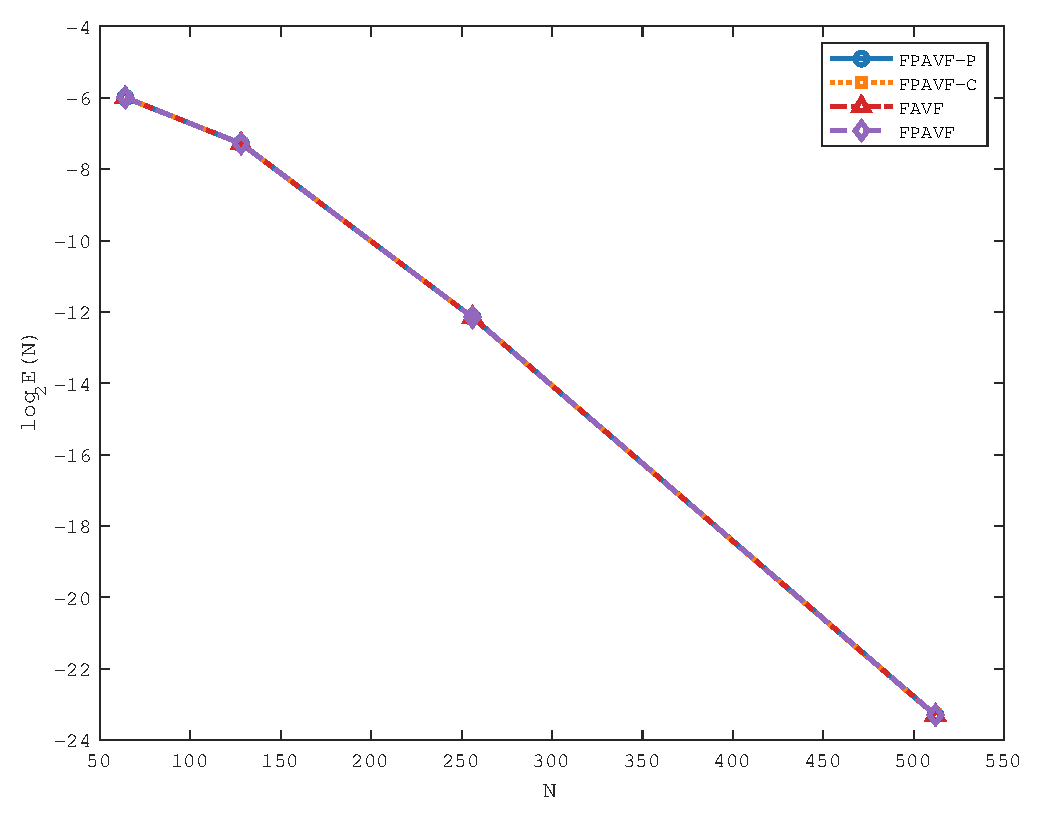
\includegraphics[width=0.35\textwidth]{./figure/exp1_s1.5.eps}
% %\centerline{($b$) Spatial accuracy with $\tau = 10^{-3}.$}
% }\subfigure[$N=128$]{ \centering
% 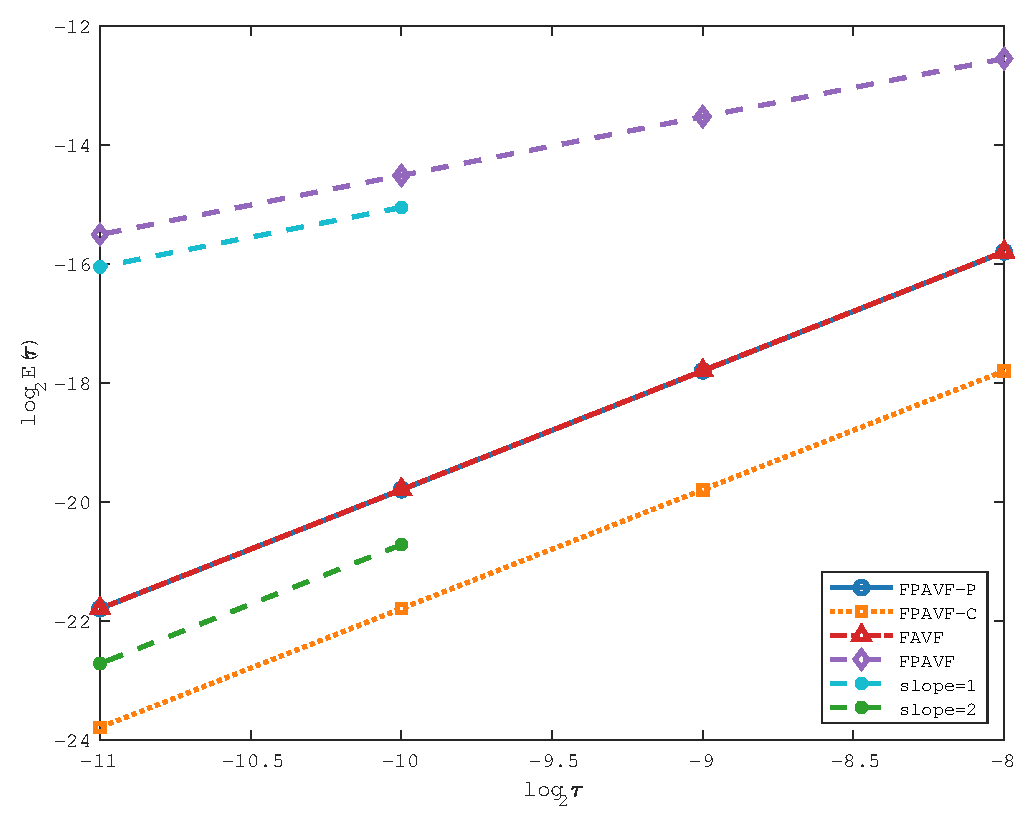
\includegraphics[width=0.35\textwidth]{./figure/exp1_t1.5.eps}
% %\centerline{($a$) Temporal accuracy with $N=128.$}
% }\caption{$\alpha=1.5$时四种方案的收敛阶(例\ref{ex:2}).} \label{fig:1}
% \end{center}
% \end{figure}

% \begin{figure}[H]
% \begin{center}
% \subfigure[$\tau=1/1000$]{ \centering
% 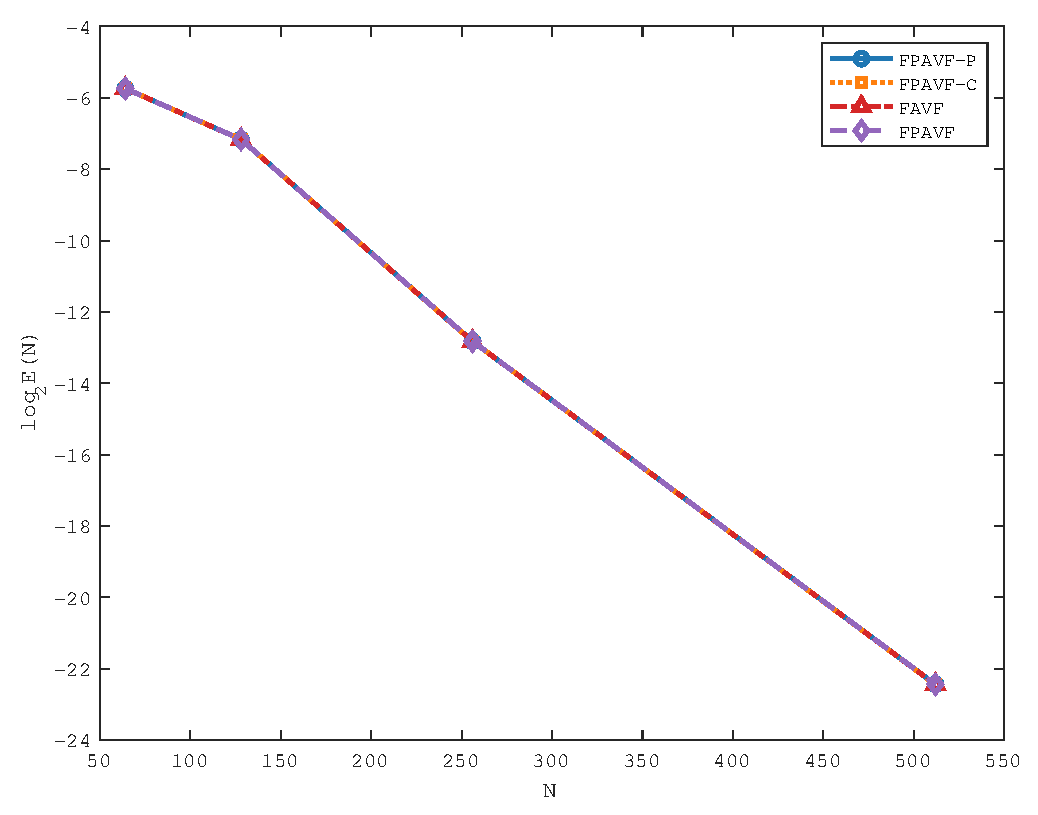
\includegraphics[width=0.35\textwidth]{./figure/exp1_s2.eps}
% %\centerline{($b$) Spatial accuracy with $\tau = 10^{-3}.$}
% }\subfigure[$N=128$]{ \centering
% 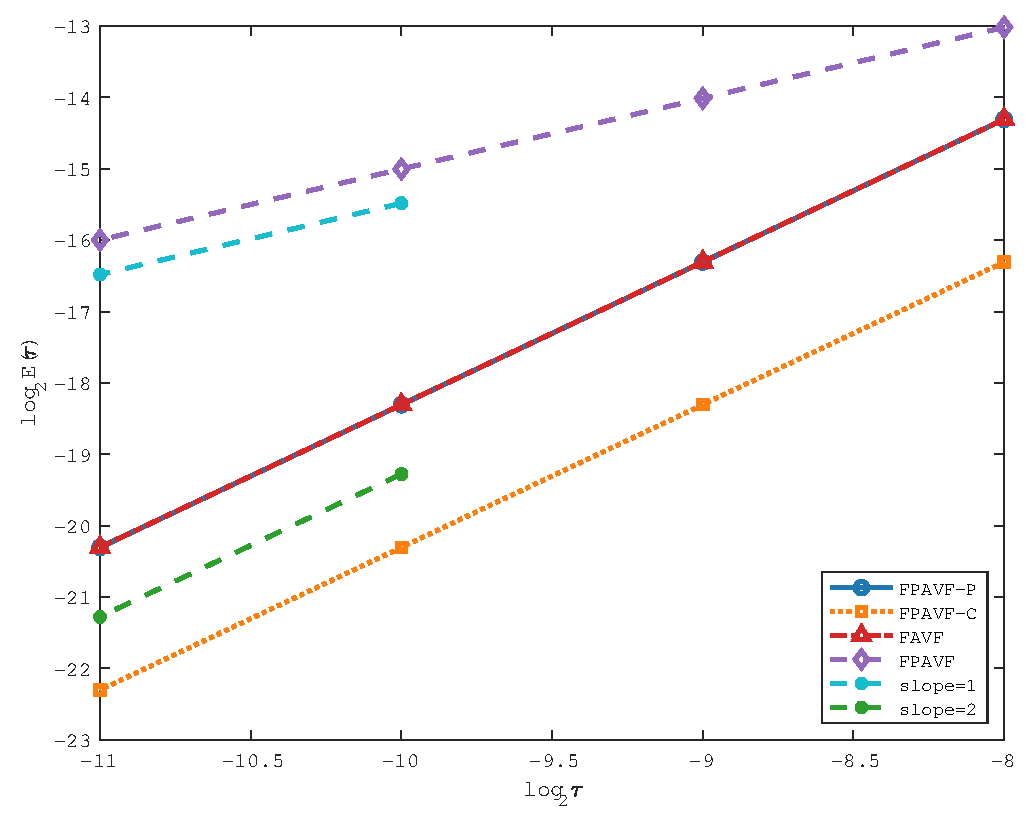
\includegraphics[width=0.35\textwidth]{./figure/exp1_t2.eps}
% %\centerline{($a$) Temporal accuracy with $N=128.$}
% }\caption{$\alpha=2$时四种方案的收敛阶(例\ref{ex:2}).} \label{fig:2}
% \end{center}
% \end{figure}

% 现在关注现有方法的守恒性能.离散能量在很长一段时间内的演化如图\ref{fig:3}所示,分别用$N=512$和$\tau=0.01$对不同的$\alpha$进行计算.尤其从$\alpha=2$的结果可以观察到,FPAVF-P、FPAVF、FAVF和FPAVF-C格式计算的离散能量均匀收敛于原始能量,而SAV方法\cite{chengConvergenceEnergyconservingScheme2022}和三级线性隐式差分格式\cite{ranLinearlyImplicitConservative2016}的性能较差.这一现象与后者是一致的,后者只保留了一种修正的能量,而不是原始的能量.

% \begin{figure}[H]
% 	\begin{center}
% 	\subfigure[$\alpha=1.3$]{ \centering
% 	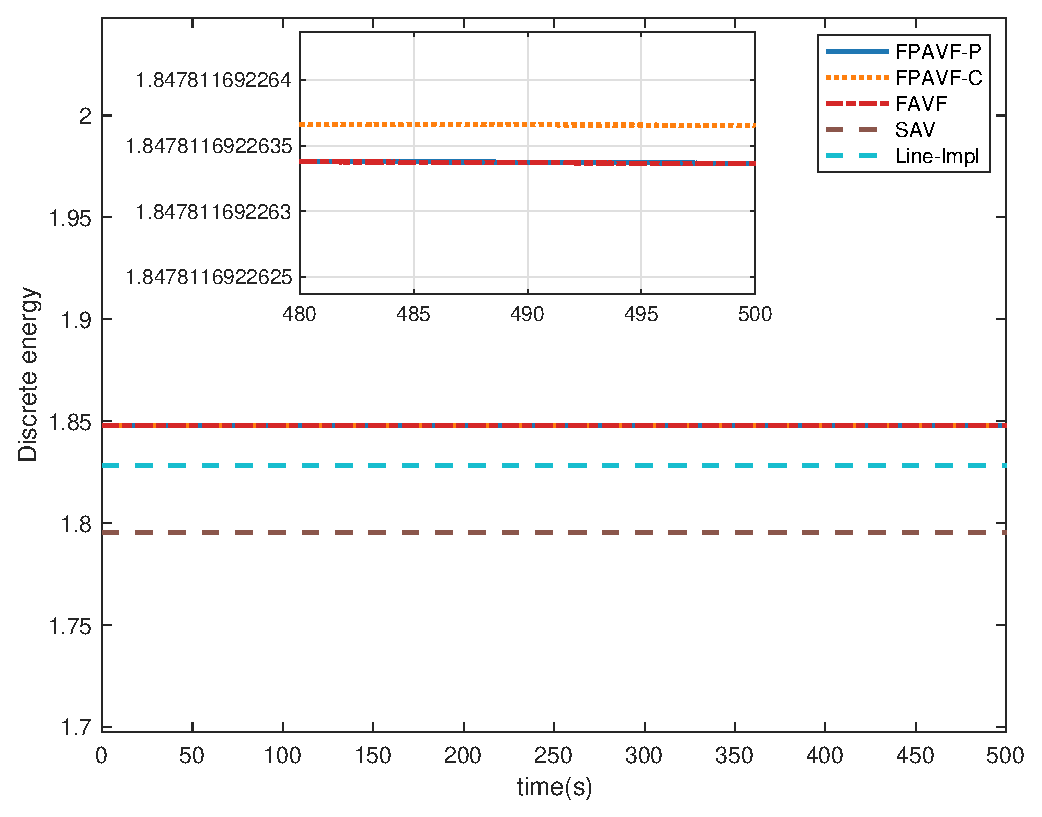
\includegraphics[width=0.4\textwidth]{./figure/exp1_H1.3.eps}
% 	%\centerline{($a$) $\alpha=1.3$}
% 	}\subfigure[$\alpha=1.6$]{ \centering
% 	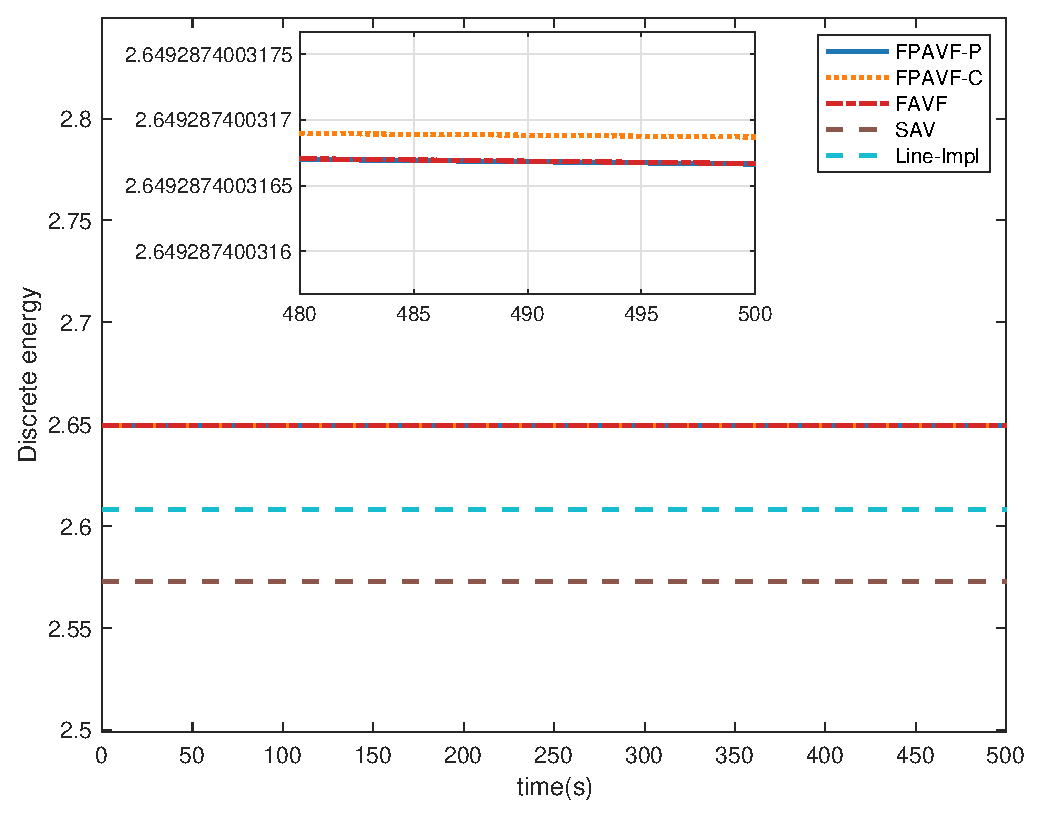
\includegraphics[width=0.4\textwidth]{./figure/exp1_H1.6.eps}
% 	%\centerline{($b$) $\alpha=1.6$}
% 	}\\
% 	\subfigure[$\alpha=1.9$]{ \centering
% 	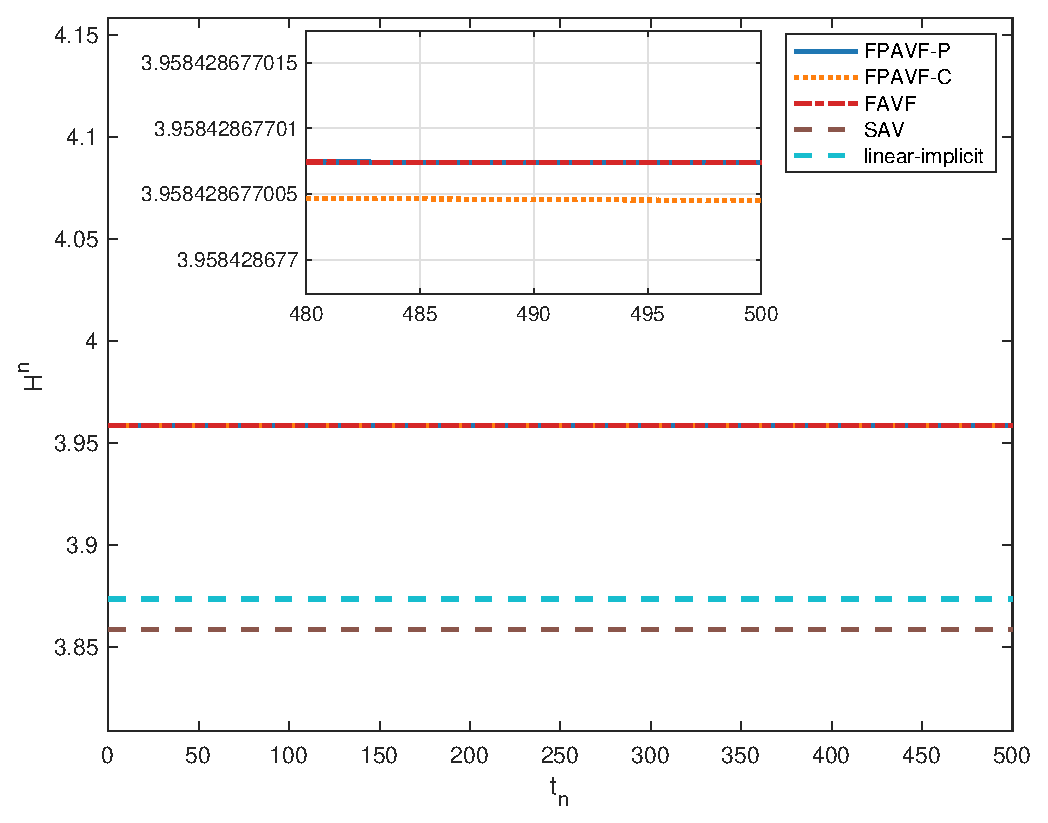
\includegraphics[width=0.4\textwidth]{./figure/exp1_H1.9.eps}
% 	%\centerline{($d$) $\alpha=2.0$}
% 	}\subfigure[$\alpha=2.0$]{ \centering
% 	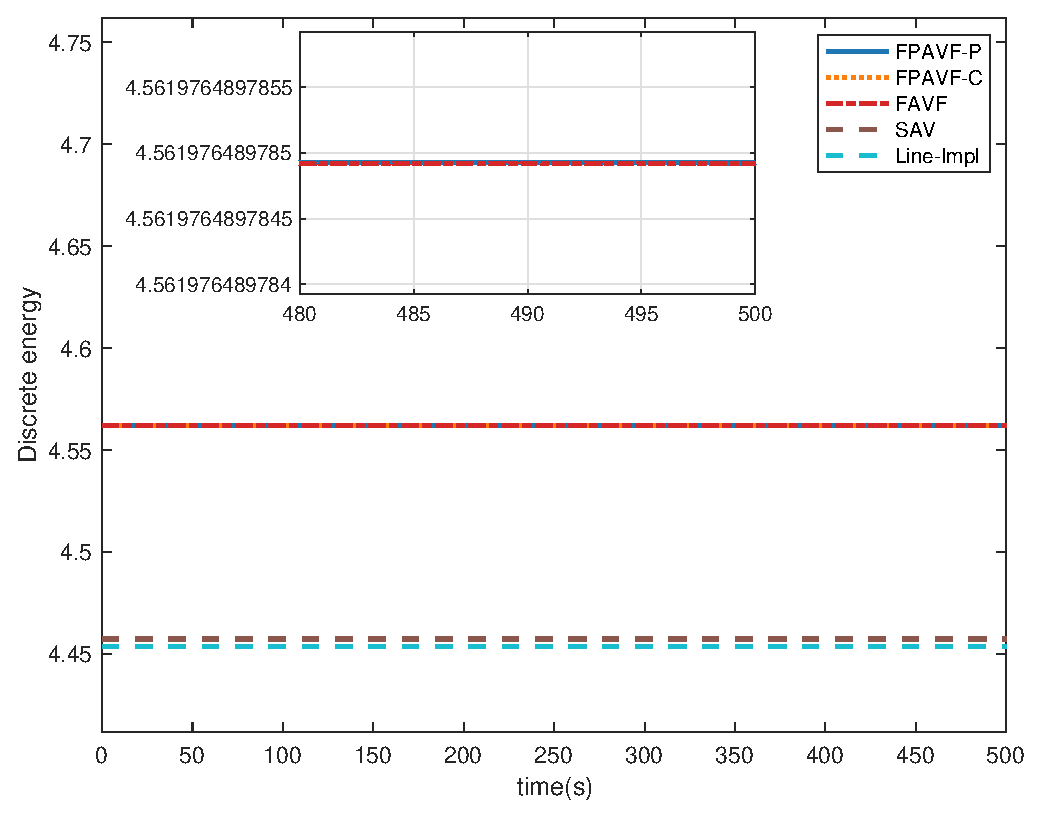
\includegraphics[width=0.4\textwidth]{./figure/exp1_H2.eps}
% 	%\centerline{($d$) $\alpha=2.0$}
% 	}\caption{$N = 512,\tau=0.01$时针对不同$\alpha$的离散能量(例\ref{ex:2}).} \label{fig:3}
% 	\end{center}
% 	\end{figure}

% 	类似地,离散质量在长时间内的演化如图\ref{Fig:4}所示.需要强调的是,SAV方法不具有质量守恒.
% 	可以看出,FPAVF-P格式对原始质量是一致收敛的,其他方法性能较差,特别是FAVF格式,三级线性隐式差分格式保留了一个修正的质量.基于FPAVF-C格式的离散质量在小范围内出现了频繁的振荡.
% \begin{figure}[H]
% 	\begin{center}
% 	 \subfigure[$\alpha=1.3$]{ \centering
% 	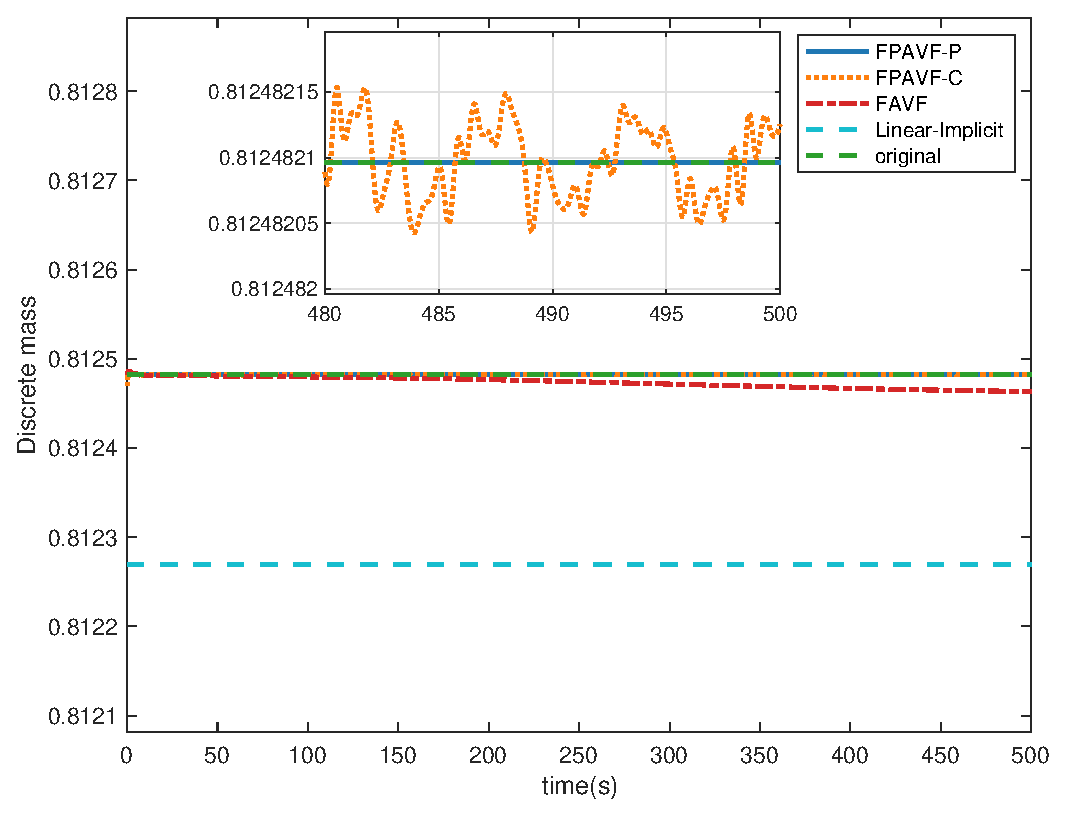
\includegraphics[width=0.4\textwidth]{./figure/exp1_M1.3.eps}
% 	%\centerline{($a$) $\alpha=1.3$}
% 	}\subfigure[$\alpha=1.6$]{ \centering
% 	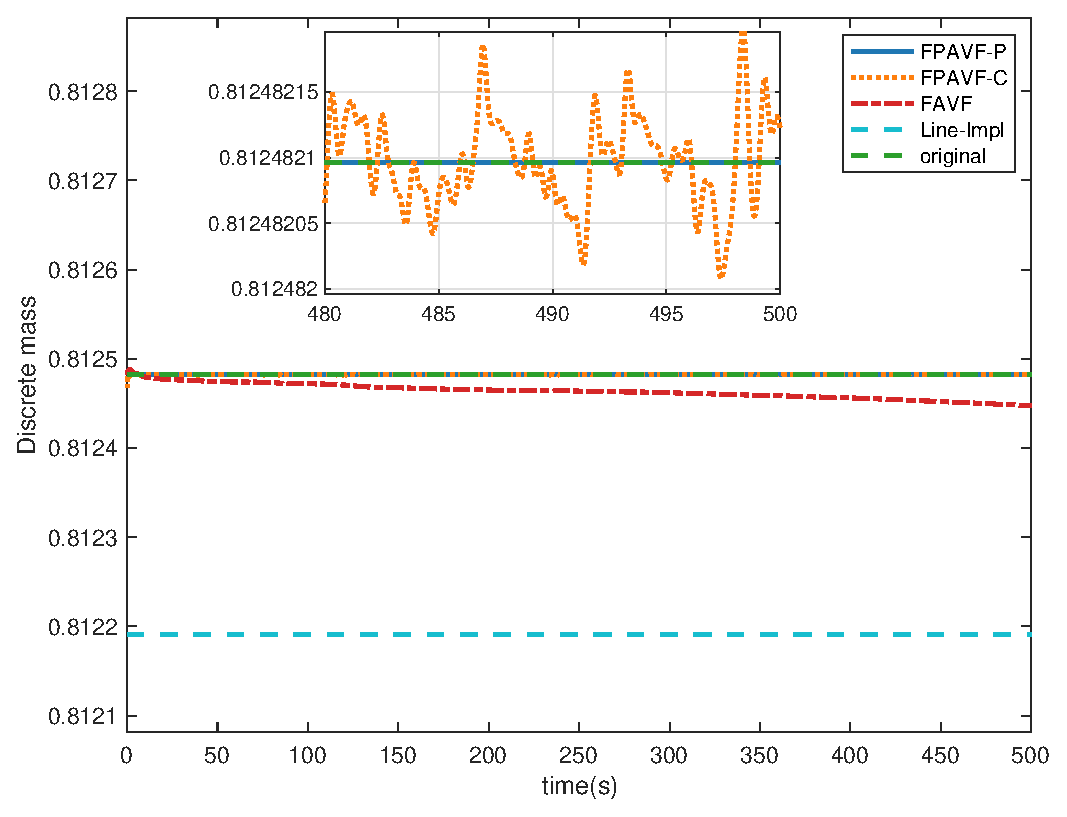
\includegraphics[width=0.4\textwidth]{./figure/exp1_M1.6.eps}
% 	%\centerline{($b$) $\alpha=1.6$}
% 	}\\
% 	 \subfigure[$\alpha=1.9$]{ \centering
% 	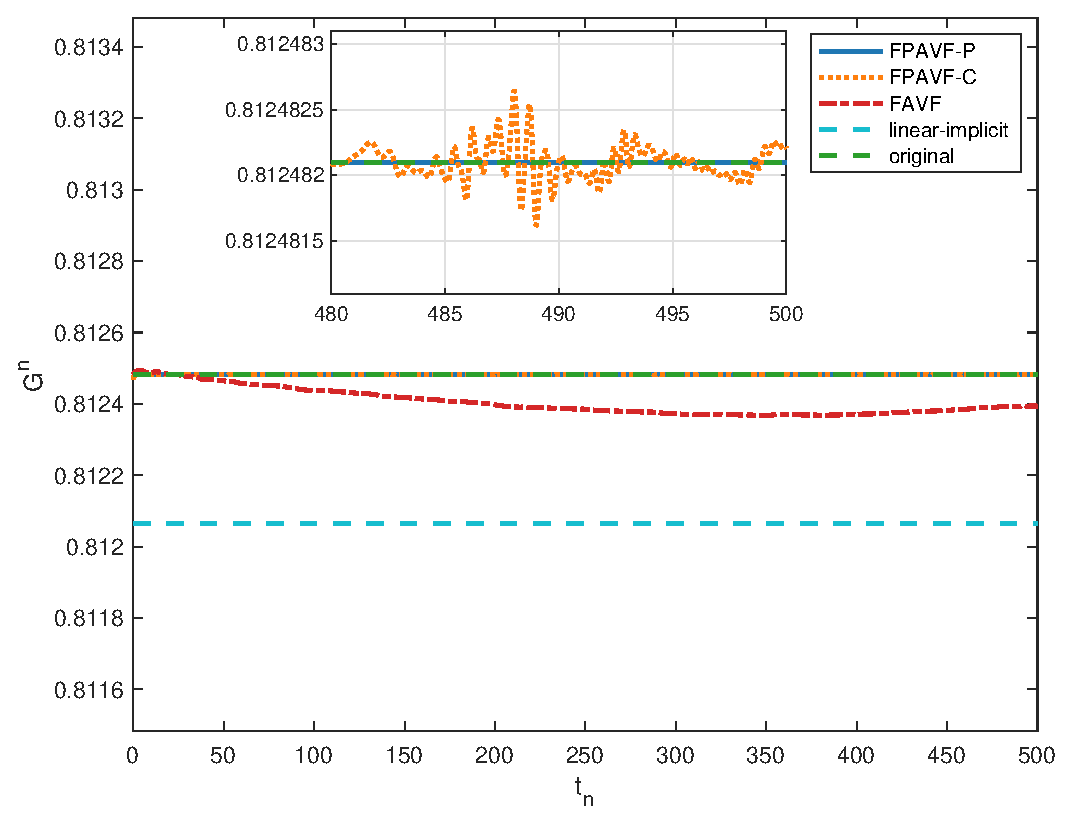
\includegraphics[width=0.4\textwidth]{./figure/exp1_M1.9.eps}
% 	%\centerline{($c$) $\alpha=1.9$}
% 	}\subfigure[$\alpha=2.0$]{ \centering
% 	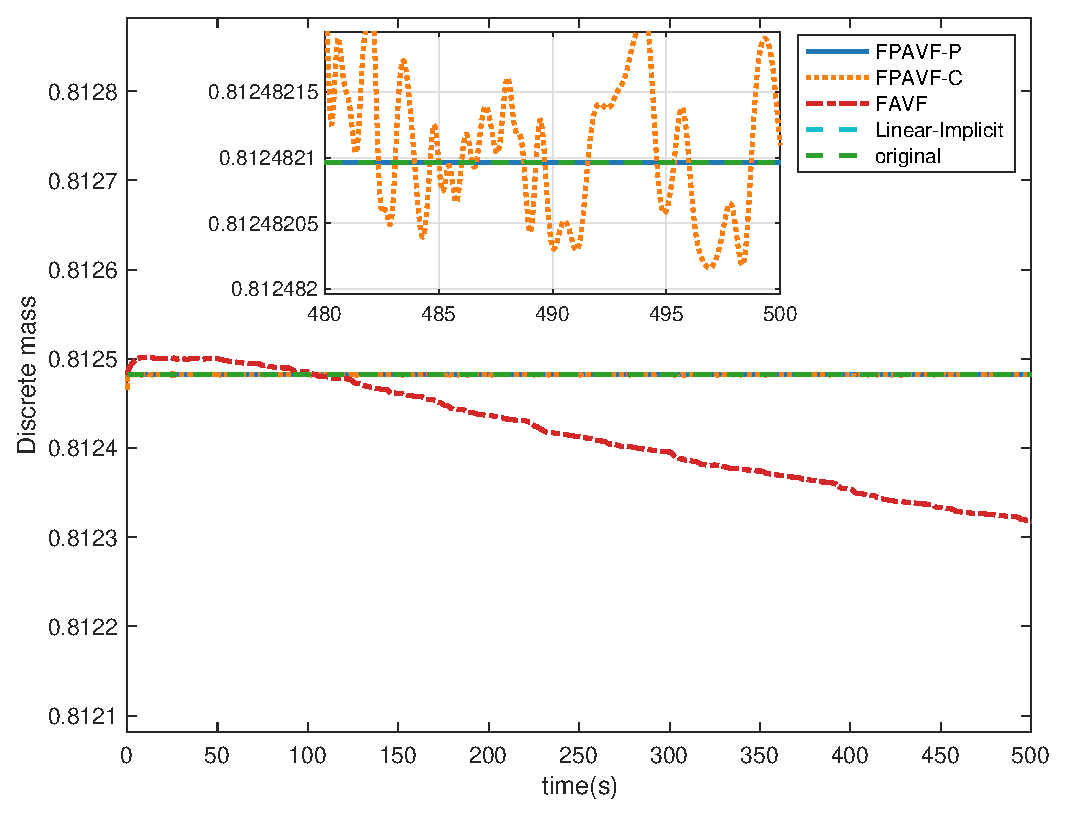
\includegraphics[width=0.4\textwidth]{./figure/exp1_M2.eps}
% 	%\centerline{($d$) $\alpha=2.0$}
% 	}\caption{$N = 512,\tau=0.01$时针对不同$\alpha$的离散质量(例\ref{ex:2}).} \label{fig:4}
% 	\end{center}
% 	\end{figure}


% 	更精确地说,对于不同的$\alpha$,离散能量$H^n$和离散质量$G^n$在不同时间$t=t_n$的值见表\ref{tab:1}-\ref{tab:4},
% 	分别取$N=512$和$\tau=0.01$.从表\ref{tab:1}可以看出,所提出的四种格式都保留了原始能量,而SAV格式和线性隐式差分格式只保留了修改后的能量.同样,从表\ref{tab:2}-\ref{tab:4}中,我们观察到FPAVF-P格式对原始质量是一致收敛的,其他方法性能较差,三级线性隐式格式只守恒修改后的质量.

% \begin{table}[H]\small
% 	\centering
% 	\caption{当$\alpha=2$时,$t=t_n$处的离散能量$H^n$(例\ref{ex:2}).}
% 	  \begin{tabular}{lllllll}
% 	  \toprule
%        $t$   &FAVF   &FPAVF   &FPAVF-C   &SAV    &Linear-Implicit   &FPAVF-P\\
% 	  \midrule
% 	  0     &4.561976489785   &4.561976489785   &4.561976489785   &4.457414815200   &4.453861069486   &4.561976489785 \\
% 	  10    &4.561976489785   &4.561976489785   &4.561976489785   &4.457414815200   &4.453861069486   &4.561976489785 \\
% 	  100   &4.561976489785   &4.561976489785   &4.561976489782   &4.457414815197   &4.453861069489   &4.561976489785 \\
% 	  200   &4.561976489785   &4.561976489785   &4.561976489779   &4.457414815195   &4.453861069492   &4.561976489785 \\
% 	  300   &4.561976489785   &4.561976489785   &4.561976489776   &4.457414815192   &4.453861069494   &4.561976489785 \\
% 	  400   &4.561976489785   &4.561976489785   &4.561976489772   &4.457414815190   &4.453861069497   &4.561976489785 \\
% 	  500   &4.561976489785   &4.561976489785   &4.561976489768   &4.457414815187   &4.453861069500   &4.561976489785 \\
% 	  \midrule
% 	  \multicolumn{7}{r}{Original energy:~4.56197648980619} \\
% 	  \bottomrule
% 	  \end{tabular}\label{tab:1}%
%   \end{table}%


% \begin{table}[H]\small
% 	\centering
% 	\caption{当$\alpha=1.3$时,$t=t_n$处的离散质量$G^n$(例\ref{ex:2}).}
% 	  \begin{tabular}{llllll}
% 	  \toprule
% $t$   &FAVF   &FPAVF   &FPAVF-C   &Linear-Implicit   &FPAVF-P\\
% 	  \midrule
% 	  0     &0.812482096011643   &0.812486108372853   &0.812481093228288   &0.812269212105079   &0.812482096009232 \\
% 	  10    &0.812481652913507   &0.815448411130831   &0.812482228623069   &0.812269212105449   &0.812482096009234 \\
% 	  100   &0.812479701090339   &0.815337307670638   &0.812482081439882   &0.812269212105119   &0.812482096009236 \\
% 	  200   &0.812476755660814   &0.815352772611703   &0.812482091028916   &0.812269212105298   &0.812482096009256 \\
% 	  300   &0.812471706145304   &0.815369448311709   &0.812482102752682   &0.812269212105193   &0.812482096009262 \\
% 	  400   &0.812466871593141   &0.815375406648485   &0.812482112407629   &0.812269212105361   &0.812482096009263 \\
% 	  500   &0.812463332390332   &0.815391313914498   &0.812482125179718   &0.812269212105409   &0.812482096009261 \\
% 	  \midrule
% 	  \multicolumn{6}{r}{Original mass:~0.812482096009503} \\
% 	  \bottomrule
% 	  \end{tabular}\label{tab:2}%
%   \end{table}%


% \begin{table}[H]\small
% 	\centering
% 	\caption{当$\alpha=1.6$时,$t=t_n$处的离散质量$G^n$(例\ref{ex:2}).}
% 	  \begin{tabular}{llllll}
% 	  \toprule
% $t$   &FAVF   &FPAVF   &FPAVF-C   &Linear-Implicit   &FPAVF-P\\
% 	  \midrule
% 	  0     &0.812482096014526   &0.812487932904355   &0.812480637459791   &0.812191342790779   &0.812482096009232 \\
% 	  10    &0.812479542844467   &0.815290680597744   &0.812482338980161   &0.812191342790869   &0.812482096009234 \\
% 	  100   &0.812471993678066   &0.814964610988901   &0.812482077830270   &0.812191342790519   &0.812482096009245 \\
% 	  200   &0.812465076996841   &0.814934135072654   &0.812482168949170   &0.812191342790438   &0.812482096009252 \\
% 	  300   &0.812461964307183   &0.815026734196011   &0.812482132284732   &0.812191342790211   &0.812482096009255 \\
% 	  400   &0.812456227758388   &0.815045189971354   &0.812482132454783   &0.812191342790067   &0.812482096009255 \\
% 	  500   &0.812447472460440   &0.815097180030255   &0.812482122664758   &0.812191342789578   &0.812482096009251 \\
% 	  \midrule
% 	  \multicolumn{6}{r}{Original mass:~0.812482096009503} \\
% 	  \bottomrule
% 	  \end{tabular}\label{tab:3}%
%   \end{table}%


% \begin{table}[H]\small
% 	\centering
% 	\caption{当$\alpha=2$时,$t=t_n$处的离散质量$G^n$(例\ref{ex:2}).}
% 	  \begin{tabular}{llllll}
% 	  \toprule
% $t$   &FAVF   &FPAVF   &FPAVF-C   &Linear-Implicit   &FPAVF-P\\
% 	  \midrule
% 	  0     &0.812482096027426   &0.812492566135382   &0.812479480708946   &0.812007279829162   &0.812482096009232 \\
% 	  10    &0.812501574603936   &0.815690689466538   &0.812482208549750   &0.812007279829185   &0.812482096009233 \\
% 	  100   &0.812485179319911   &0.815559529804266   &0.812482224295188   &0.812007279829068   &0.812482096009234 \\
% 	  200   &0.812436598720768   &0.815737264057778   &0.812482177481325   &0.812007279828906   &0.812482096009234 \\
% 	  300   &0.812395565737519   &0.815914179675223   &0.812482122649446   &0.812007279828999   &0.812482096009235 \\
% 	  400   &0.812353830841431   &0.816227202656059   &0.812482101787071   &0.812007279828969   &0.812482096009235 \\
% 	  500   &0.812317849493374   &0.816336221770707   &0.812482109657662   &0.812007279829037   &0.812482096009234 \\
% 	  \midrule
% 	  \multicolumn{6}{r}{Original mass:~0.812482096009503} \\
% 	  \bottomrule
% 	  \end{tabular}\label{tab:4}%
%   \end{table}%



%   基于$\alpha\ne2 $的原始能量不易计算的事实,我们从相对误差的角度验证了离散守恒定律,见图\ref{fig:5}-\ref{fig:6}.
%   这些数据再次表明,FPAVF-P方案在保留原始质量方面具有最佳性能.而随着$\alpha$的增加,其保持原始能量的性能会更好.
%   这些观察结果与我们之前的理论结果是一致的.



% \begin{figure}[H]
% \begin{center}
%  \subfigure[$\alpha=1.3$]{ \centering
% 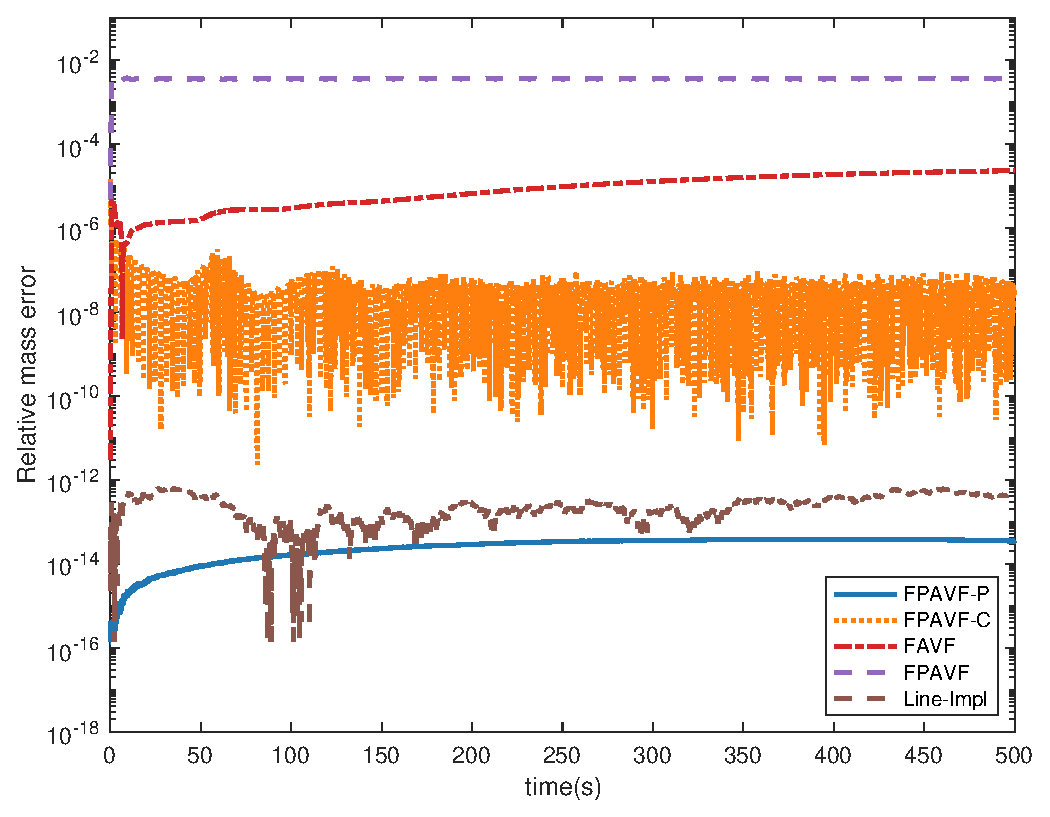
\includegraphics[width=0.3\textwidth]{./figure/exp1_RM1.3.eps}
% %\centerline{($a$) $\alpha=1.3$}
% }\subfigure[$\alpha=1.6$]{ \centering
% 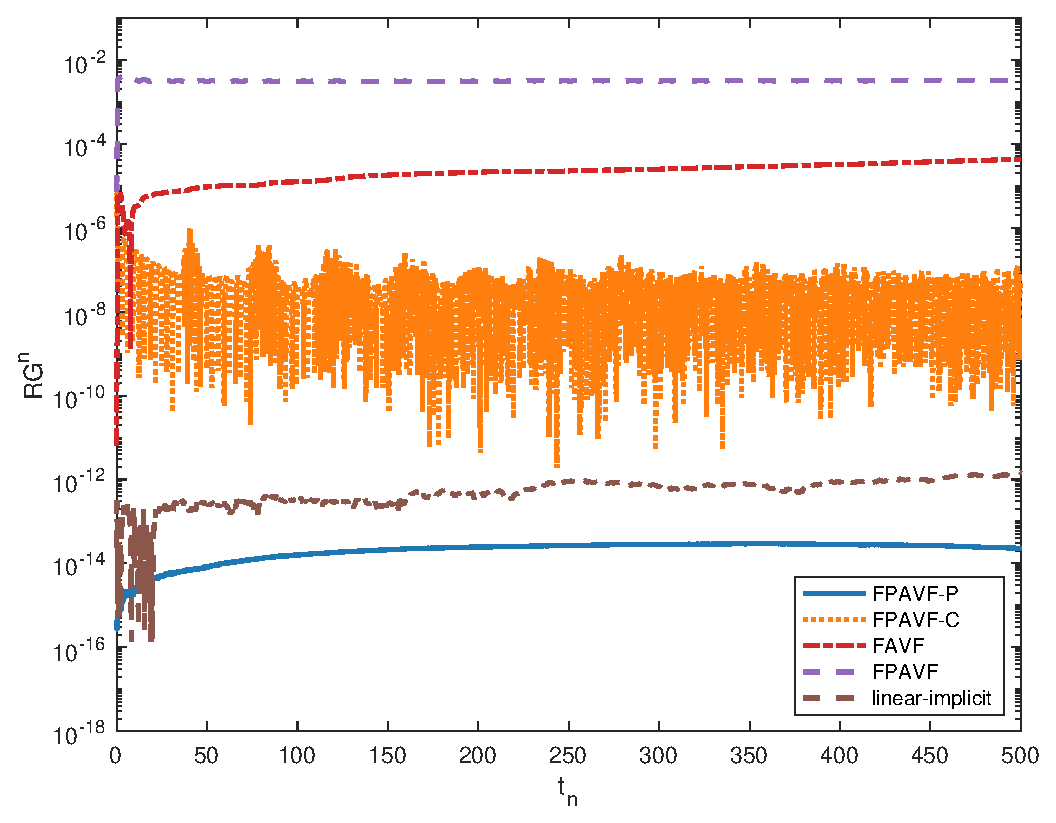
\includegraphics[width=0.3\textwidth]{./figure/exp1_RM1.6.eps}
% %\centerline{($b$) $\alpha=1.6$}
% }\subfigure[$\alpha=1.9$]{ \centering
% 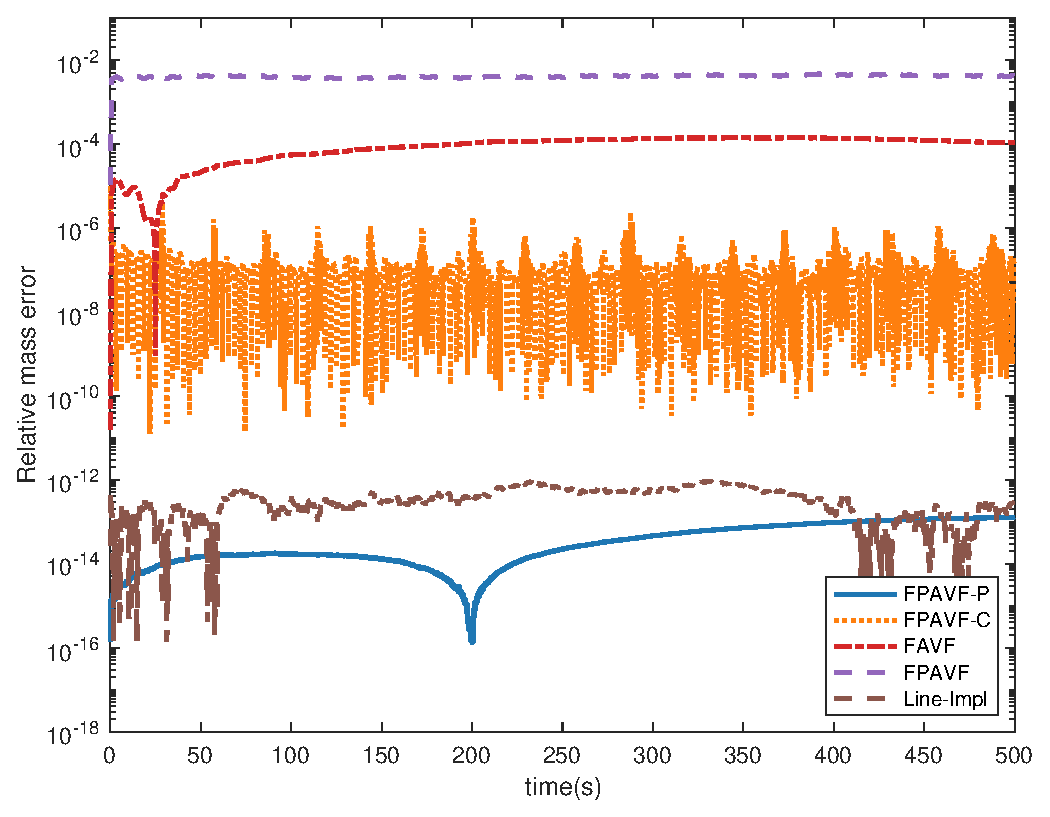
\includegraphics[width=0.3\textwidth]{./figure/exp1_RM1.9.eps}
% %\centerline{($c$) $\alpha=1.9$}
% }\caption{$N = 512,\tau=0.01$时针对不同$\alpha$的相对离散质量误差(例\ref{ex:2}).} \label{fig:5}
% \end{center}
% \end{figure}

% \begin{figure}[H]
% \begin{center}
%  \subfigure[$\alpha=1.3$]{ \centering
% 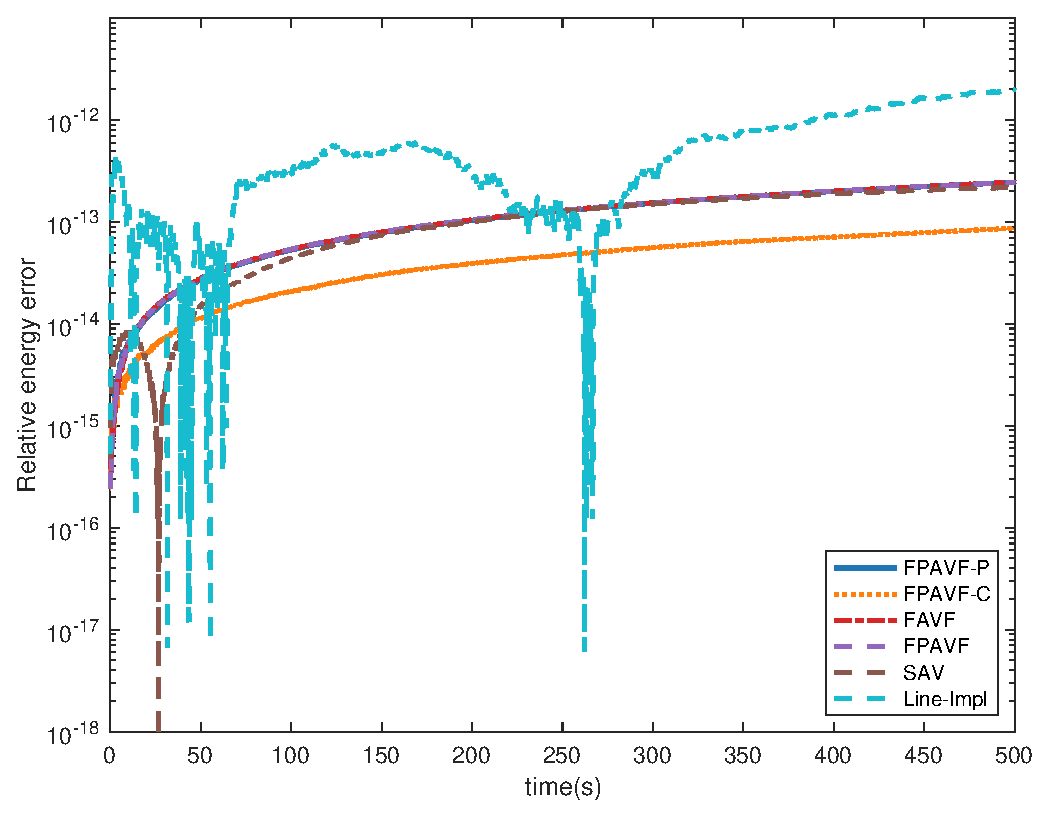
\includegraphics[width=0.3\textwidth]{./figure/exp1_RH1.3.eps}
% %\centerline{($a$) $\alpha=1.3$}
% }\subfigure[$\alpha=1.6$]{ \centering
% 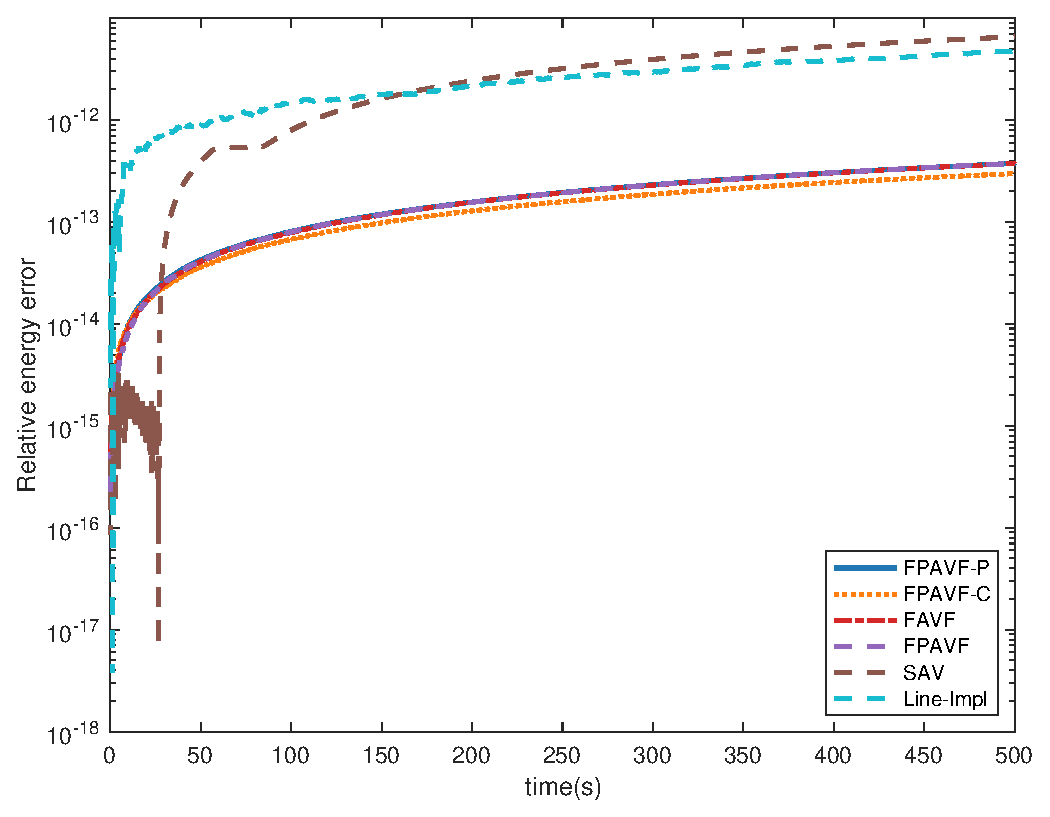
\includegraphics[width=0.3\textwidth]{./figure/exp1_RH1.6.eps}
% %\centerline{($b$) $\alpha=1.6$}
% } \subfigure[$\alpha=1.9$]{ \centering
% 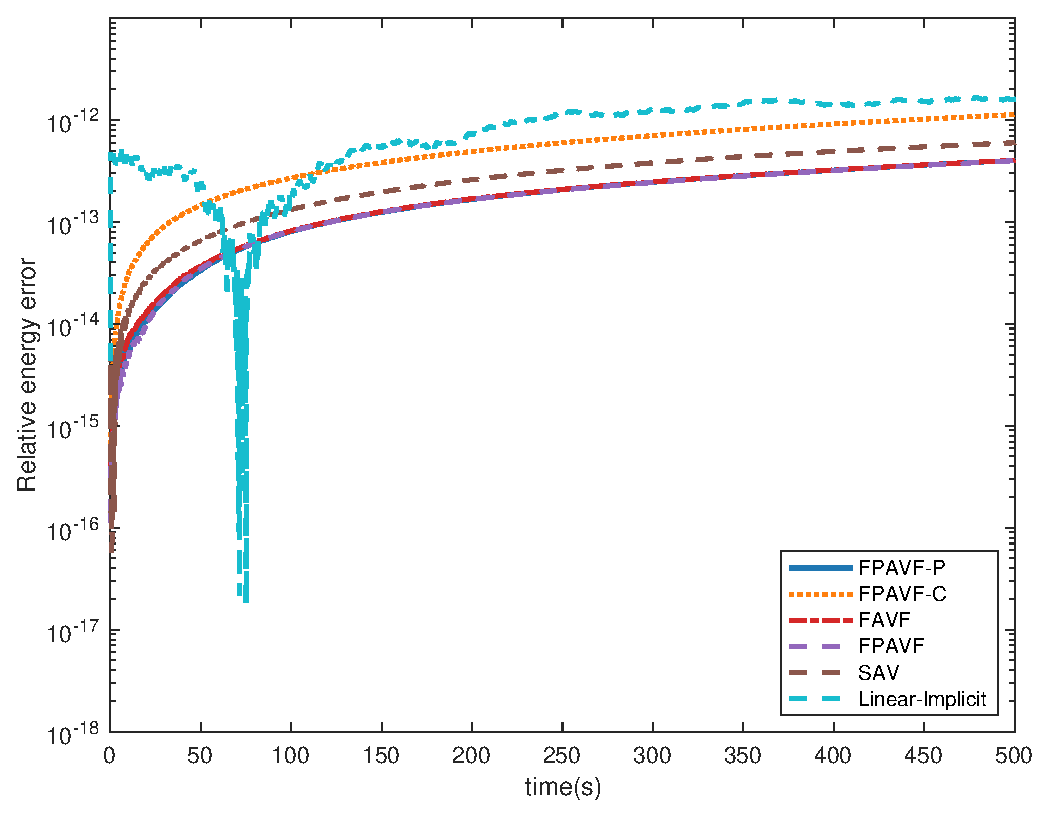
\includegraphics[width=0.3\textwidth]{./figure/exp1_RH1.9.eps}
% %\centerline{($c$) $\alpha=1.9$}
% }\caption{$N = 512,\tau=0.01$时针对不同$\alpha$的相对离散能量误差(例\ref{ex:2}).} \label{fig:6}
% \end{center}
% \end{figure}



% \begin{example}\label{ex:4}
% 考虑具有以下初值条件的二维 NFSWEs \eqref{eq:s1} 
% \begin{equation}\label{eq_110}
% u(x,y, 0)=\mbox{sech}\left(x^2+y^2\right), u_t(x,y, 0)=\sin (x+y) \mbox{sech}\left(-2(x^2+y^2)\right), (x,y,t)\in  \Omega\times[0, T],
% \end{equation}
% 其中 $\Omega=[-5,5] \times[-5,5]$.
% \end{example}


% 与一维情况类似,我们首先计算$T=1$时$\alpha=1.5$和$\alpha=2.0$时FPAVF-P、FPAVF、FAVF和FPAVF-P格式的收敛阶数.\ref{fig:7}-\ref{fig:8}所示为误差的变化.我们可以清楚地观察到,四种方案都具有空间谱精度,FPAVF方案具有一阶精度,其他方案在时间上具有二阶精度.
% \begin{figure}[H]
% \begin{center}
% \subfigure[$\tau=1/1000$]{ \centering
% 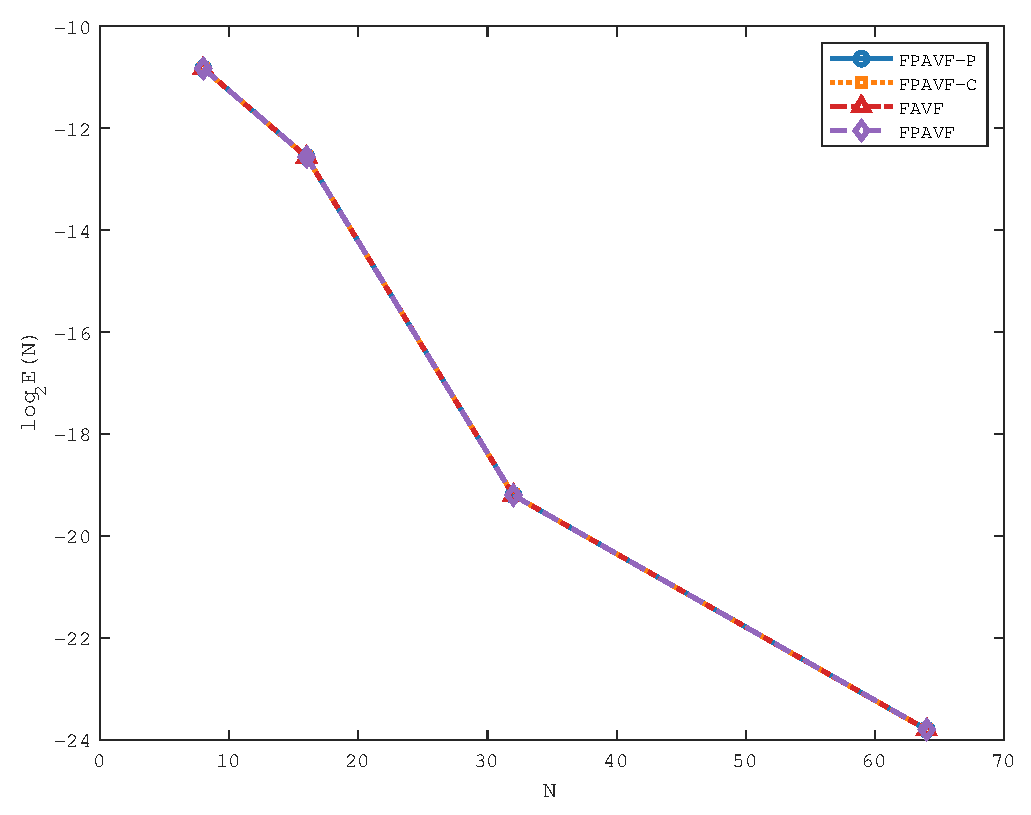
\includegraphics[width=0.35\textwidth]{./figure/exp2_s1.5.eps}
% %\centerline{($b$) Spatial accuracy with $\tau = 10^{-3}.$}
% }\subfigure[$N=16$]{ \centering
% 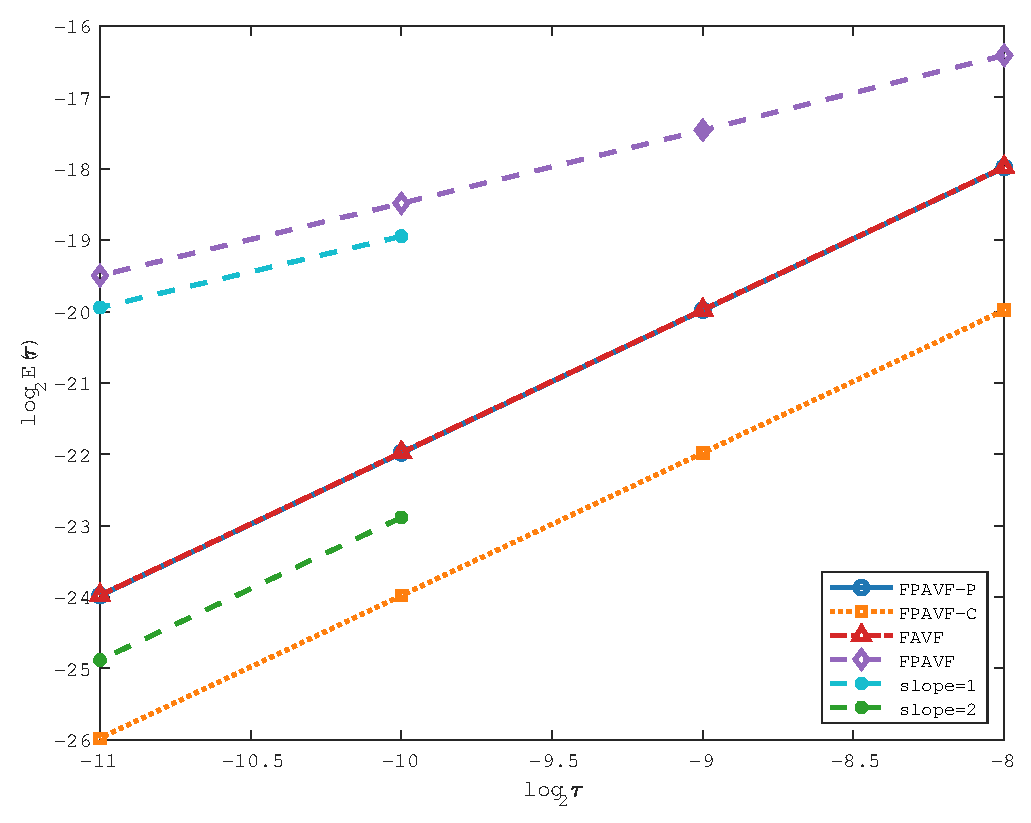
\includegraphics[width=0.35\textwidth]{./figure/exp2_t1.5.eps}
% %\centerline{($a$) Temporal accuracy with $N=128.$}
% }\caption{$\alpha=1.5$时四种方案的收敛阶(例\ref{ex:4}).} \label{fig:7}
% \end{center}
% \end{figure}

% \begin{figure}[H]
% \begin{center}
% \subfigure[$\tau=1/1000$]{ \centering
% 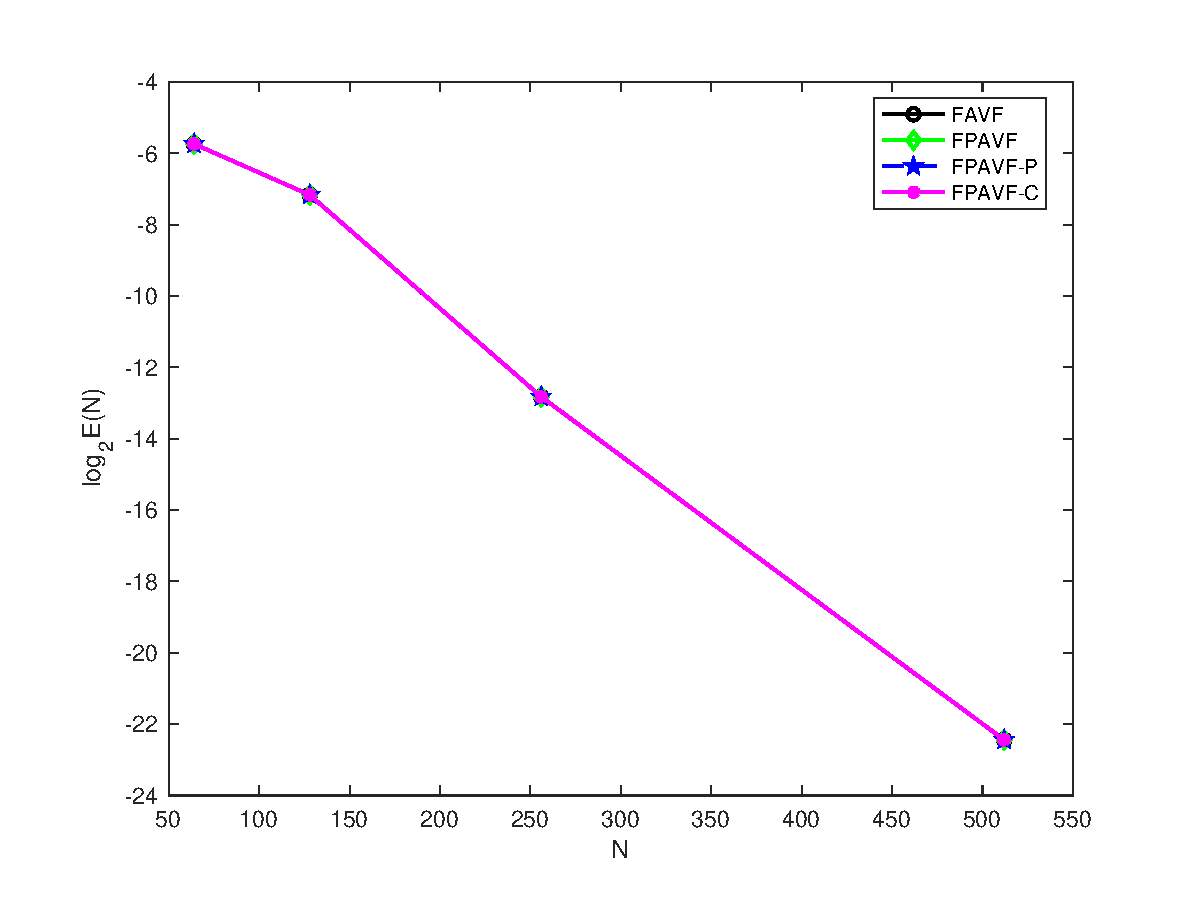
\includegraphics[width=0.35\textwidth]{./figure/exp2_s2.eps}
% %\centerline{($b$) Spatial accuracy with $\tau = 10^{-3}.$}
% }\subfigure[$N=16$]{ \centering
% 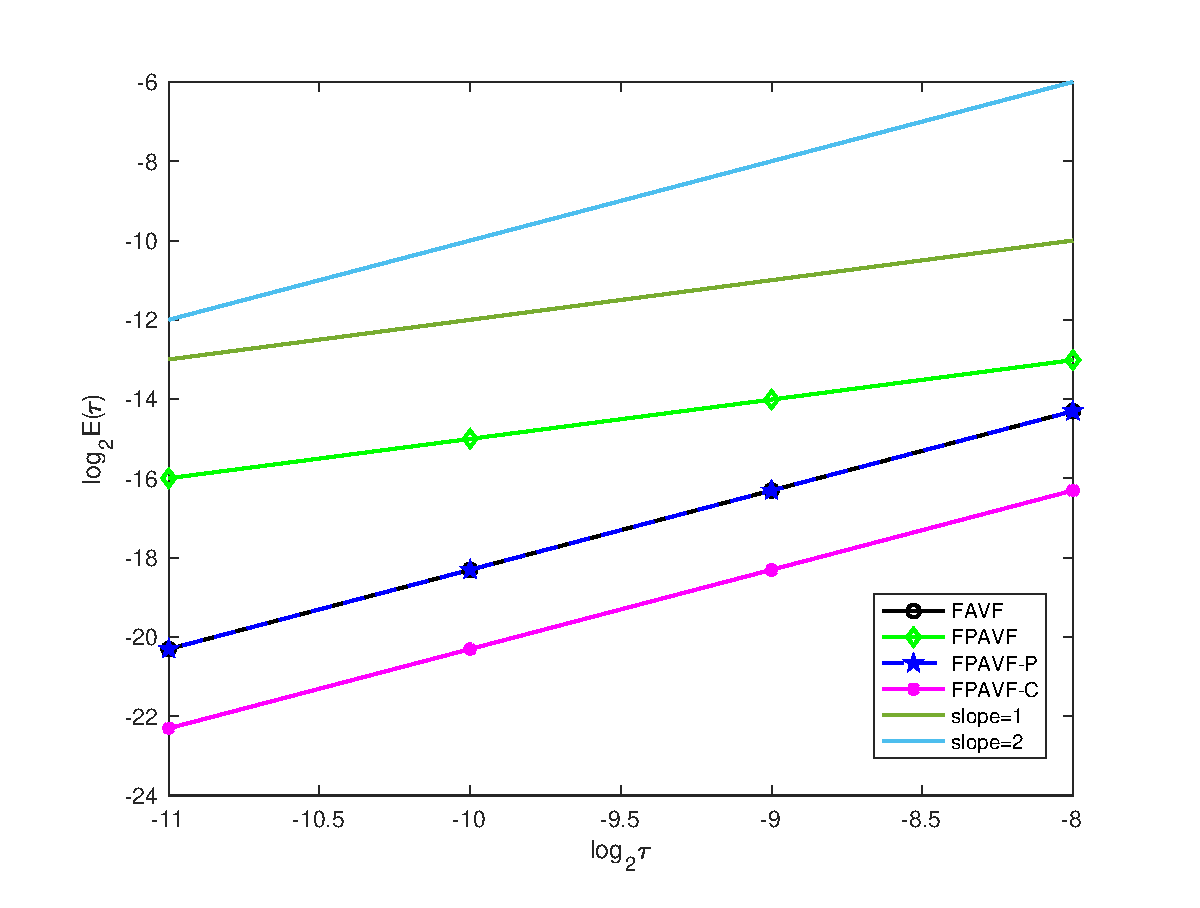
\includegraphics[width=0.35\textwidth]{./figure/exp2_t2.eps}
% %\centerline{($a$) Temporal accuracy with $N=128.$}
% }\caption{$\alpha=2$时四种方案的收敛阶(例\ref{ex:4}).} \label{fig:8}
% \end{center}
% \end{figure}


% 为了与现有方法进行结构保存能力的比较,我们首先计算了原始质量和能量.
% 注意到原始质量$G(t)$与$\alpha$无关,通过高斯数值积分,我们得到任意$\alpha$的原始质量$G(0)=3.14159265323701$.同样,我们可以得到原始能量$E(0)=3.22697078976648$, $\alpha=2$.
% 的FPAVF-P、FAVF和FPAVF-C格式的性能.离散质量和离散能量在很长一段时间内的演化如图\ref{fig:9}-\ref{fig:10}所示,分别用$N=64$和$\tau=0.01$对不同的$\alpha$进行计算.
% 这种离散质量和能量的相对误差随时间的变化也显示在图\ref{fig:11}-\ref{fig:12}中.
% 可以观察到FPAVF-P格式对原始质量是一致收敛的,其他三种方法性能较差,特别是FAVF格式和FPAVF格式(FPAVF格式的结果更差,这里不显示).
% 本文提出的三种方案都能很好地保持原始能量不变性,SAV方法只保留了一个修正的能量.这些现象再次证实了我们理论结果的正确性.

% \begin{figure}[H]
% 	\begin{center}
% 	 \subfigure[$\alpha=1.3$]{ \centering
% 	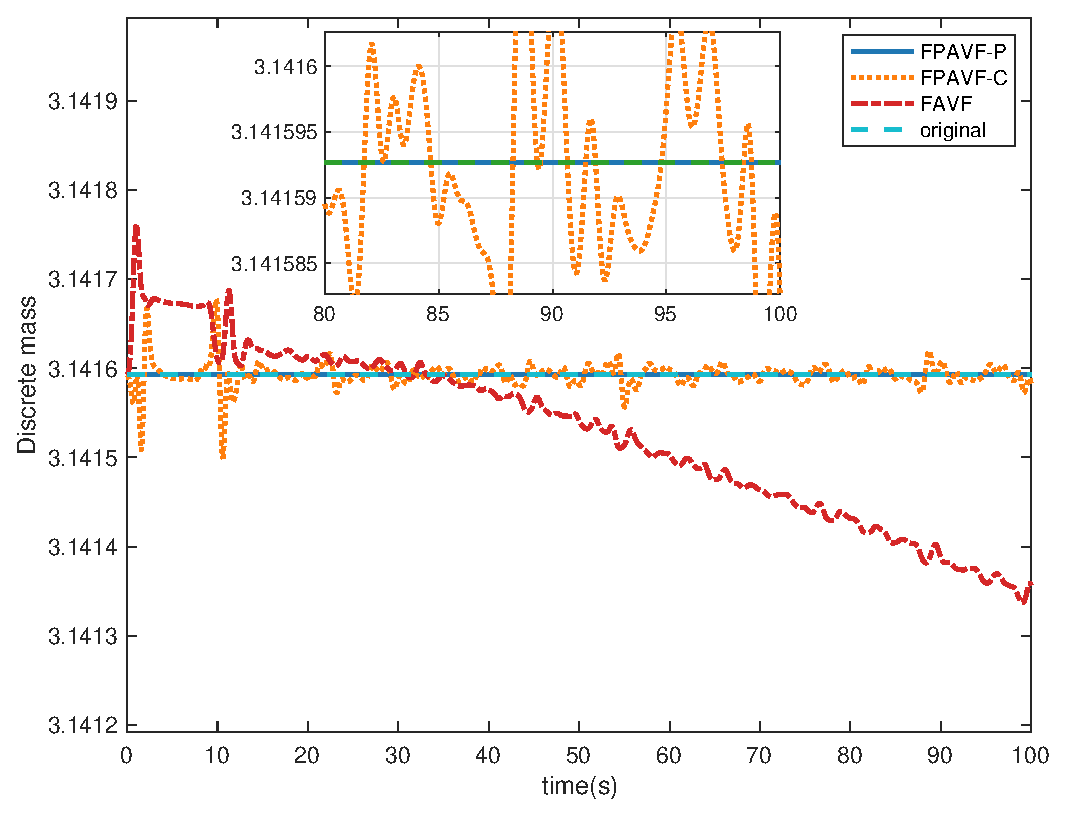
\includegraphics[width=0.3\textwidth]{./figure/exp2_M1.3.eps}
% 	%\centerline{($a$) $\alpha=1.3$}
% 	}\subfigure[$\alpha=1.6$]{ \centering
% 	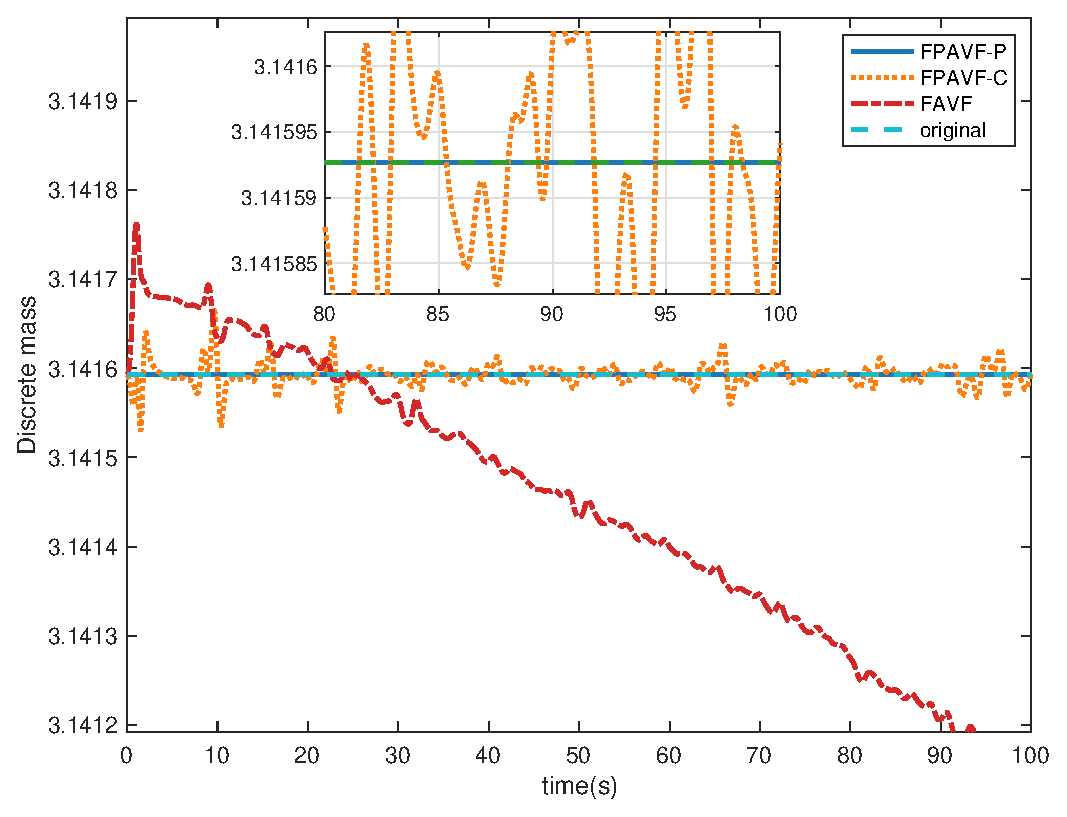
\includegraphics[width=0.3\textwidth]{./figure/exp2_M1.6.eps}
% 	%\centerline{($b$) $\alpha=1.6$}
% 	}\\
% 	 \subfigure[$\alpha=1.9$]{ \centering
% 	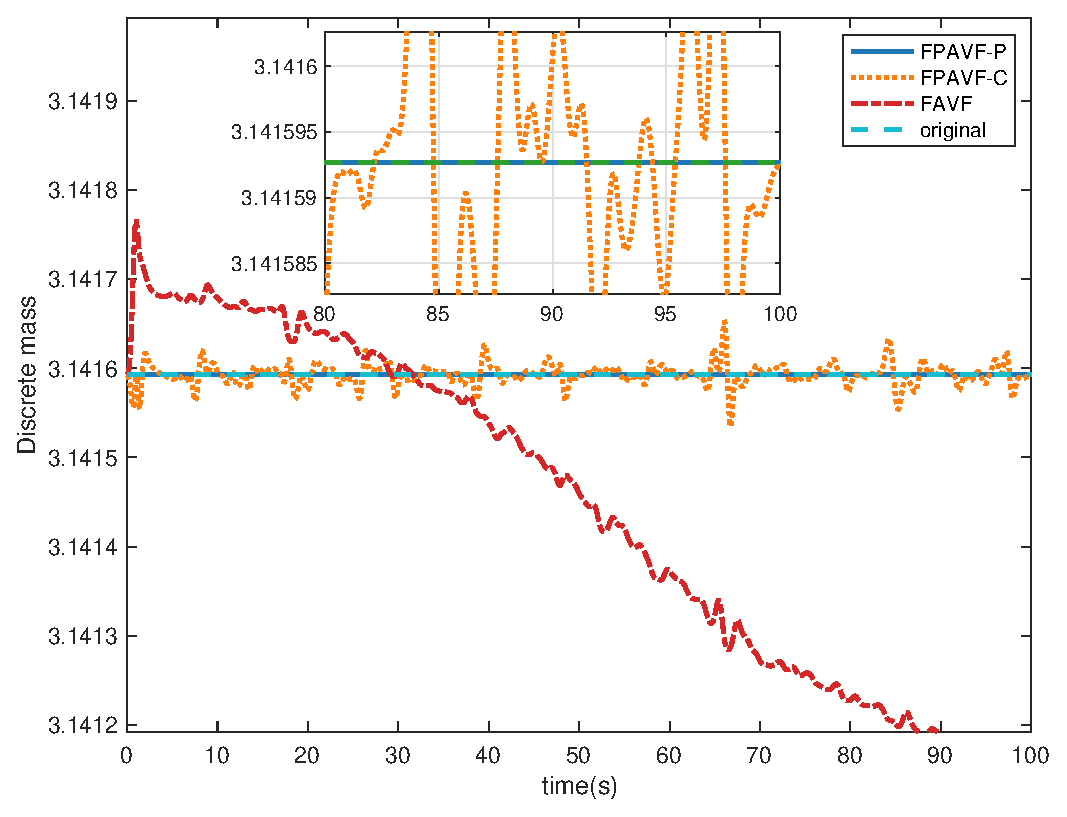
\includegraphics[width=0.3\textwidth]{./figure/exp2_M1.9.eps}
% 	%\centerline{($c$) $\alpha=1.9$}
% 	}\subfigure[$\alpha=2.0$]{ \centering
% 	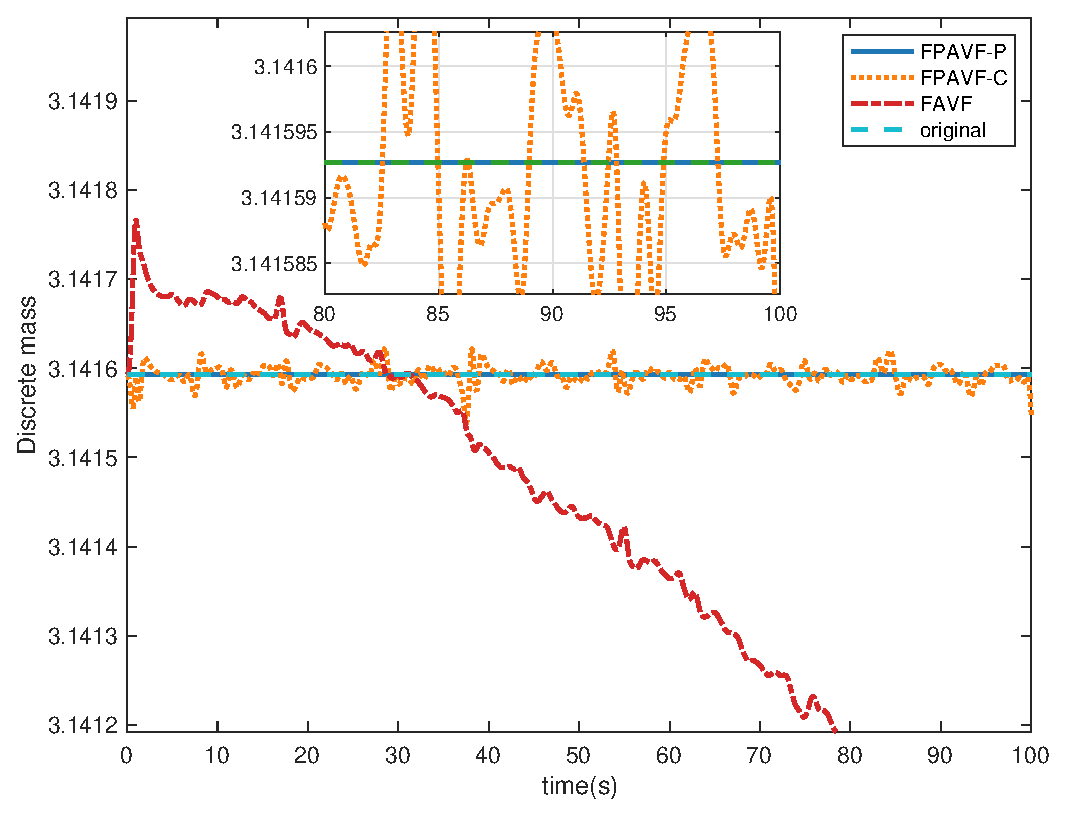
\includegraphics[width=0.3\textwidth]{./figure/exp2_M2.eps}
% 	%\centerline{($d$) $\alpha=2.0$}
% 	}\caption{$N = 64,\tau=0.01$时针对不同$\alpha$的离散质量(例\ref{ex:4}).} \label{fig:9}
% 	\end{center}
% 	\end{figure}

% \begin{figure}[H]
% 	\begin{center}
% 	\subfigure[$\alpha=1.3$]{ \centering
% 	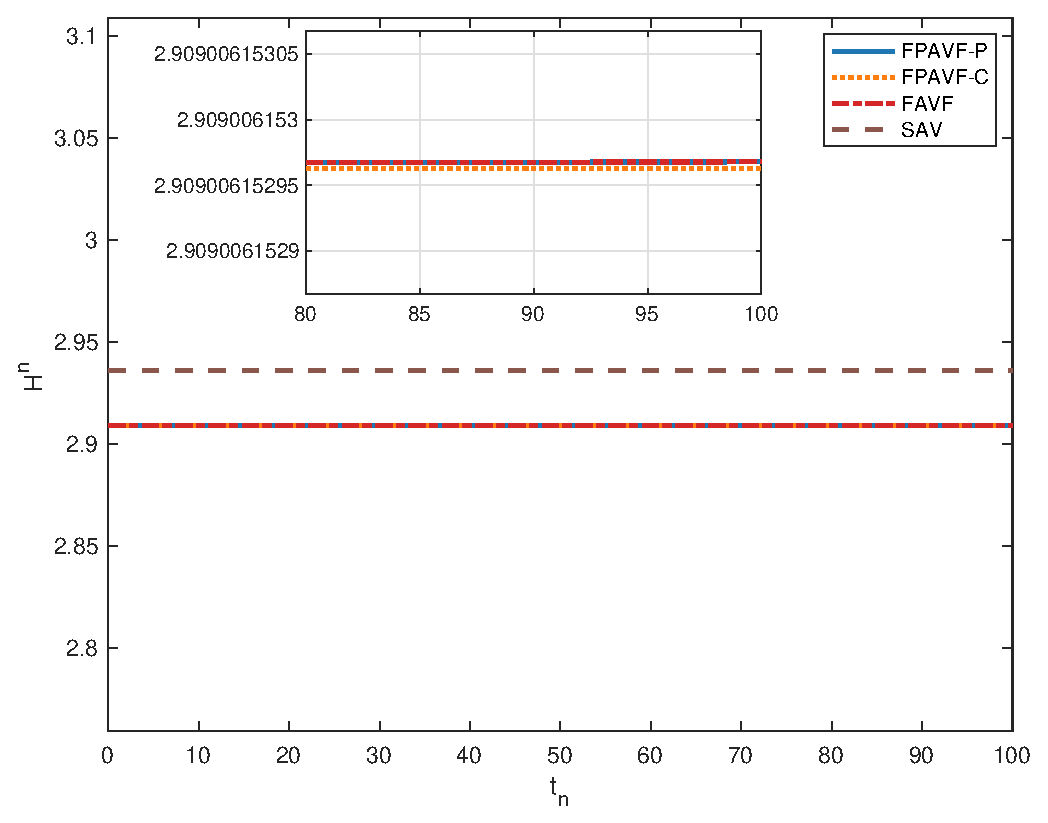
\includegraphics[width=0.3\textwidth]{./figure/exp2_H1.3.eps}
% 	%\centerline{($a$) $\alpha=1.3$}
% 	}\subfigure[$\alpha=1.6$]{ \centering
% 	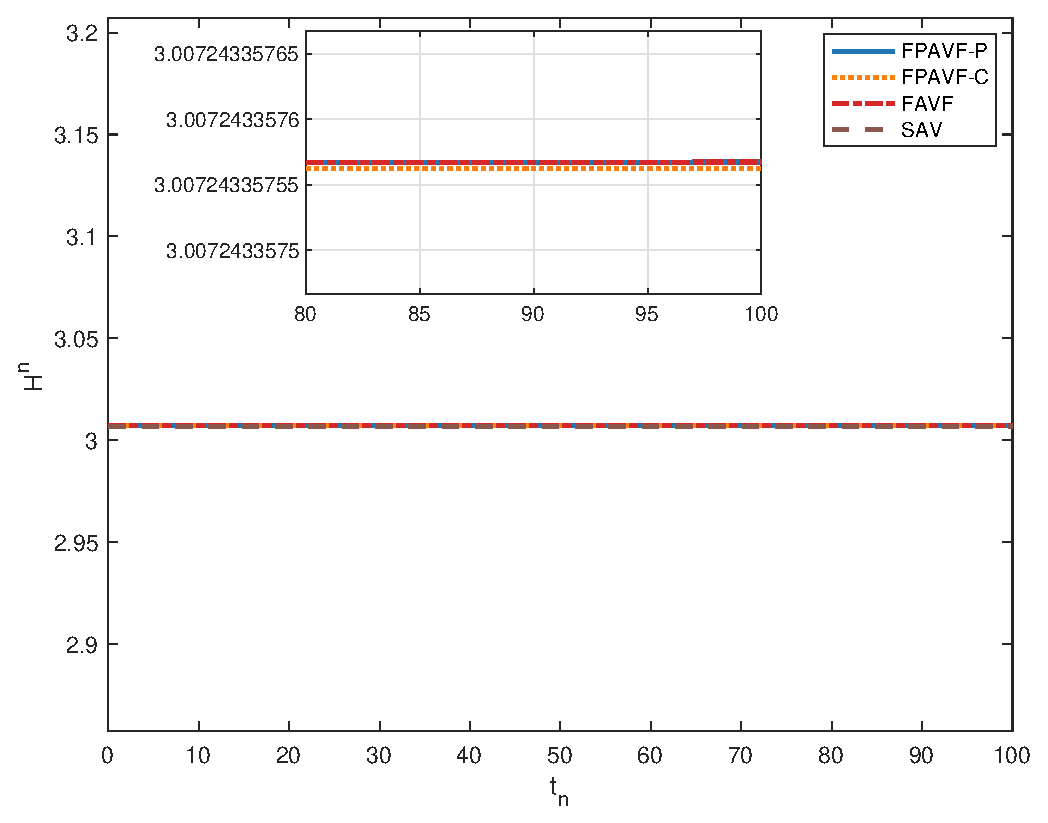
\includegraphics[width=0.3\textwidth]{./figure/exp2_H1.6.eps}
% 	%\centerline{($b$) $\alpha=1.6$}
% 	}\\
% 	\subfigure[$\alpha=1.9$]{ \centering
% 	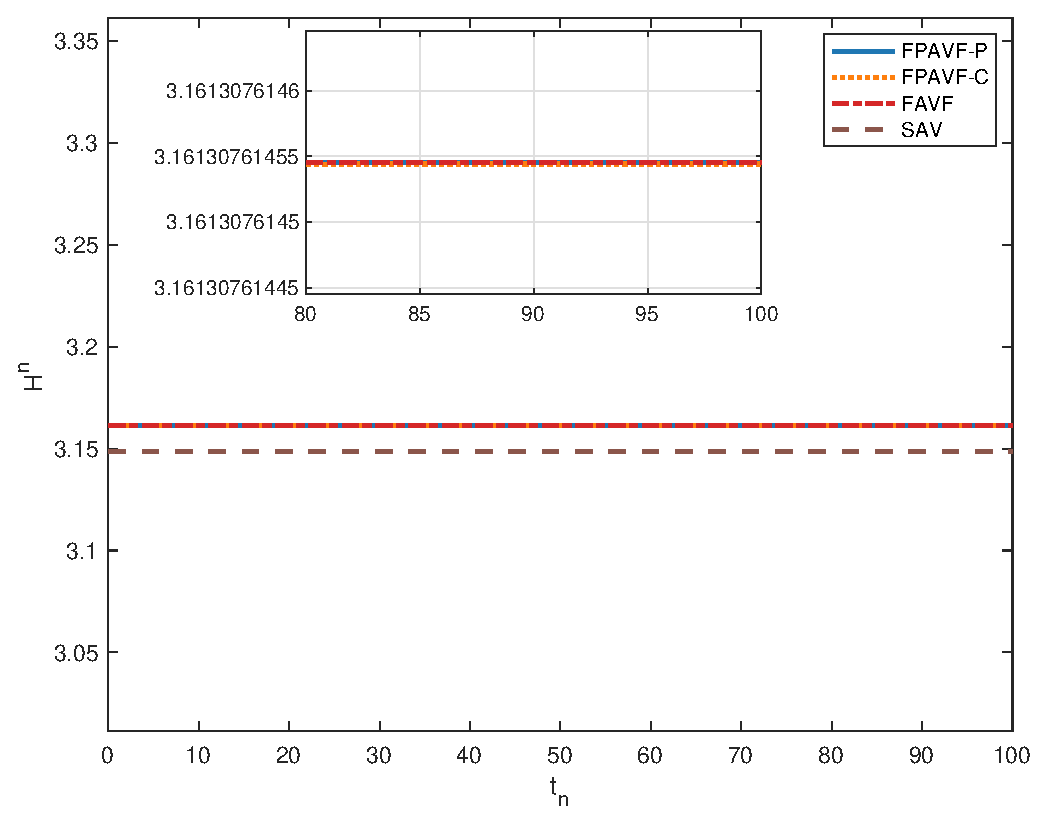
\includegraphics[width=0.3\textwidth]{./figure/exp2_H1.9.eps}
% 	%\centerline{($d$) $\alpha=2.0$}
% 	}\subfigure[$\alpha=2.0$]{ \centering
% 	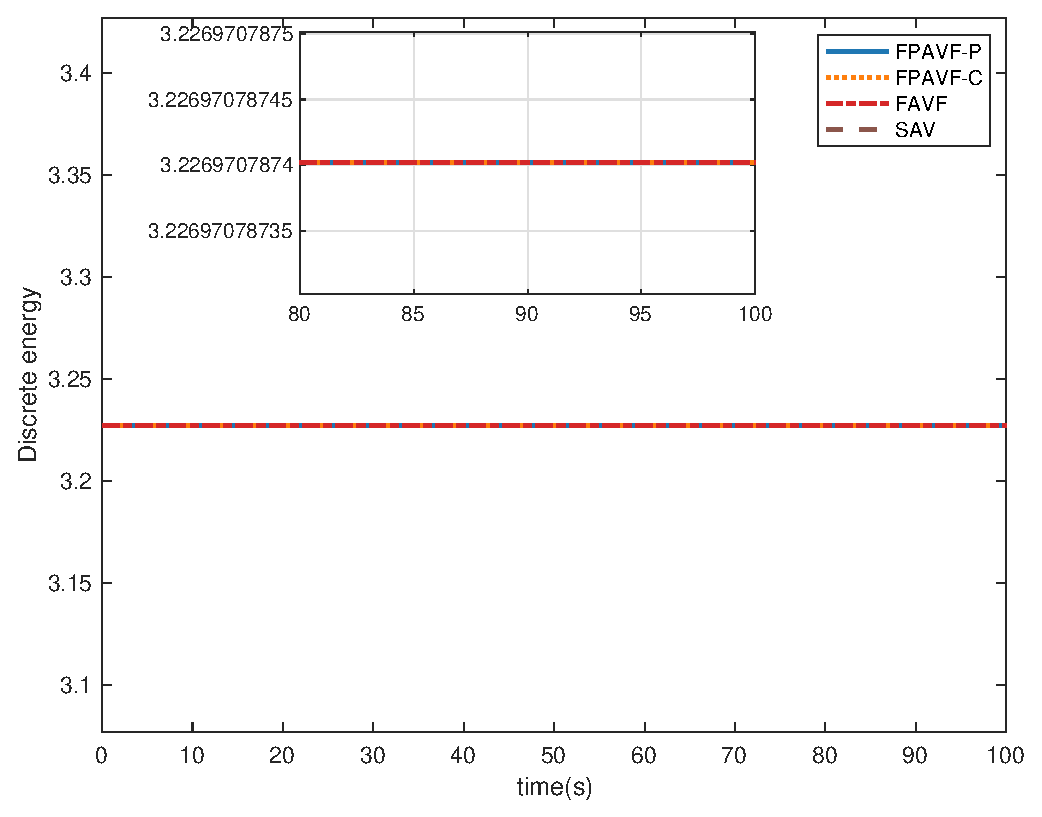
\includegraphics[width=0.3\textwidth]{./figure/exp2_H2.eps}
% 	%\centerline{($d$) $\alpha=2.0$}
% 	}\caption{$N = 64,\tau=0.01$时针对不同$\alpha$的离散能量(例\ref{ex:4}).} \label{fig:10}
% 	\end{center}
% 	\end{figure}


% \begin{figure}[H]
% \begin{center}
%  \subfigure[$\alpha=1.3$]{ \centering
% 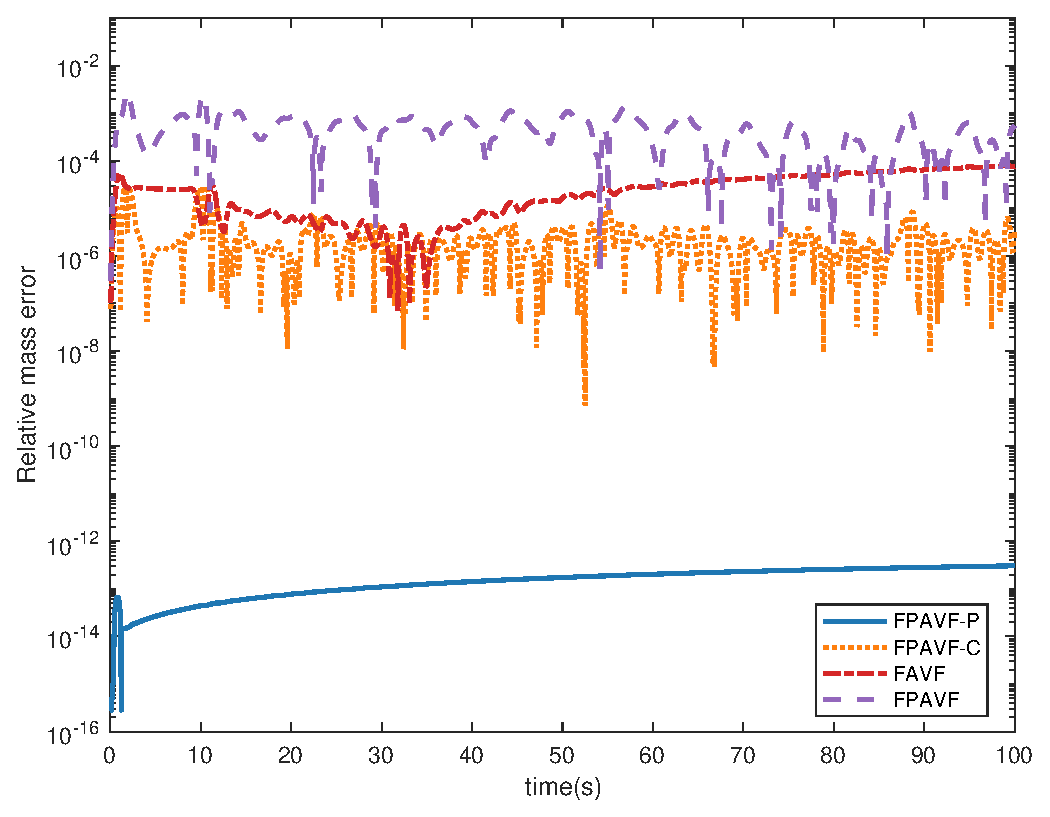
\includegraphics[width=0.3\textwidth]{./figure/exp2_RM1.3.eps}
% %\centerline{($a$) $\alpha=1.3$}
% }\subfigure[$\alpha=1.6$]{ \centering
% 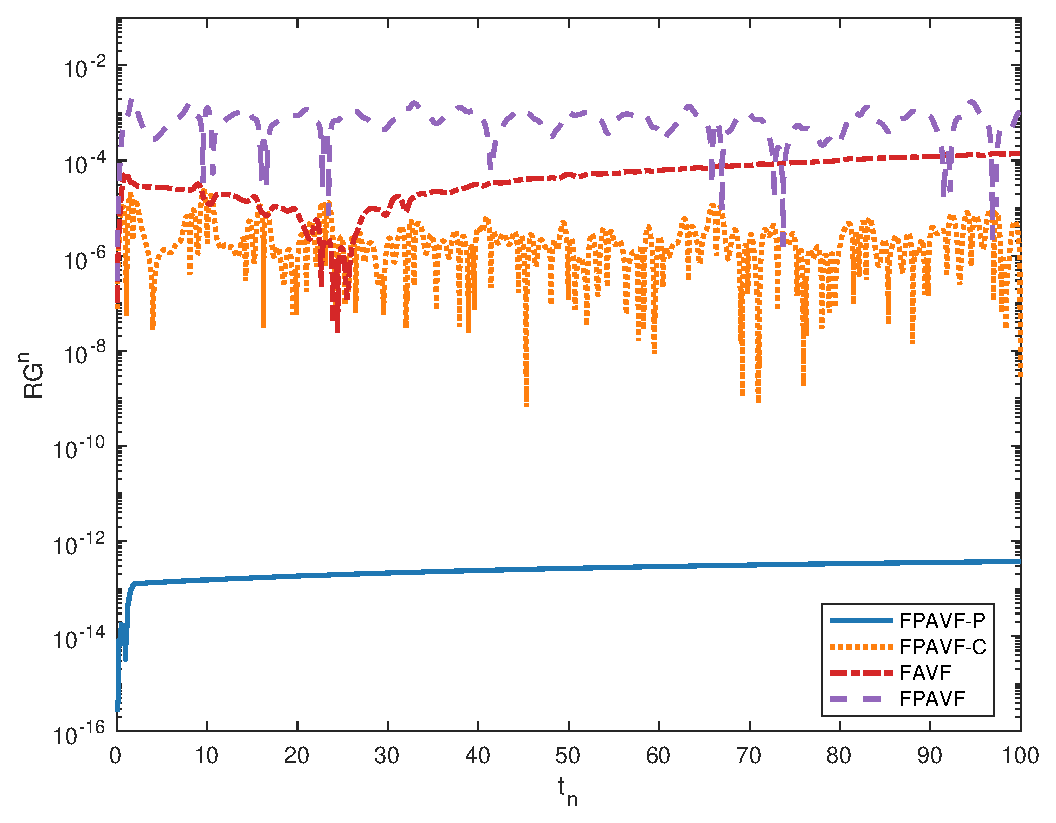
\includegraphics[width=0.3\textwidth]{./figure/exp2_RM1.6.eps}
% %\centerline{($b$) $\alpha=1.6$}
% }\subfigure[$\alpha=1.9$]{ \centering
% 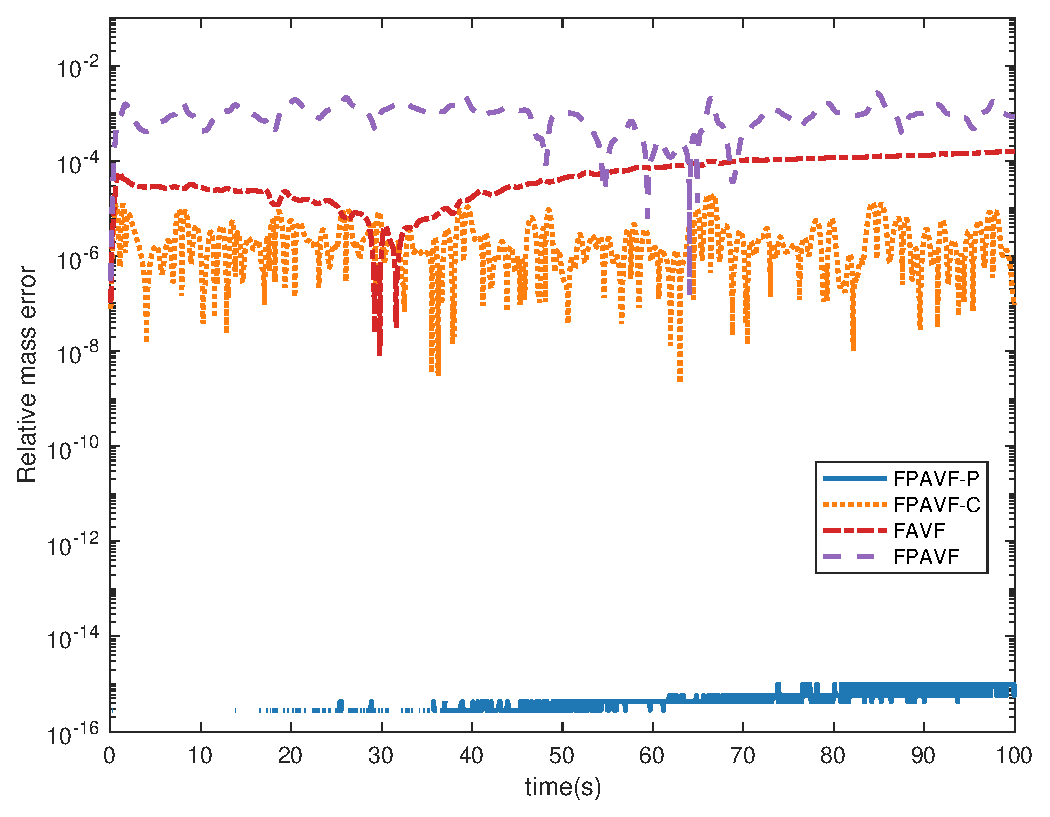
\includegraphics[width=0.3\textwidth]{./figure/exp2_RM1.9.eps}
% %\centerline{($c$) $\alpha=1.9$}
% }\caption{$N = 64,\tau=0.01$时针对不同$\alpha$的相对离散质量误差(例\ref{ex:4}).} \label{fig:11}
% \end{center}
% \end{figure}


% \begin{figure}[H]
% \begin{center}
%  \subfigure[$\alpha=1.3$]{ \centering
% 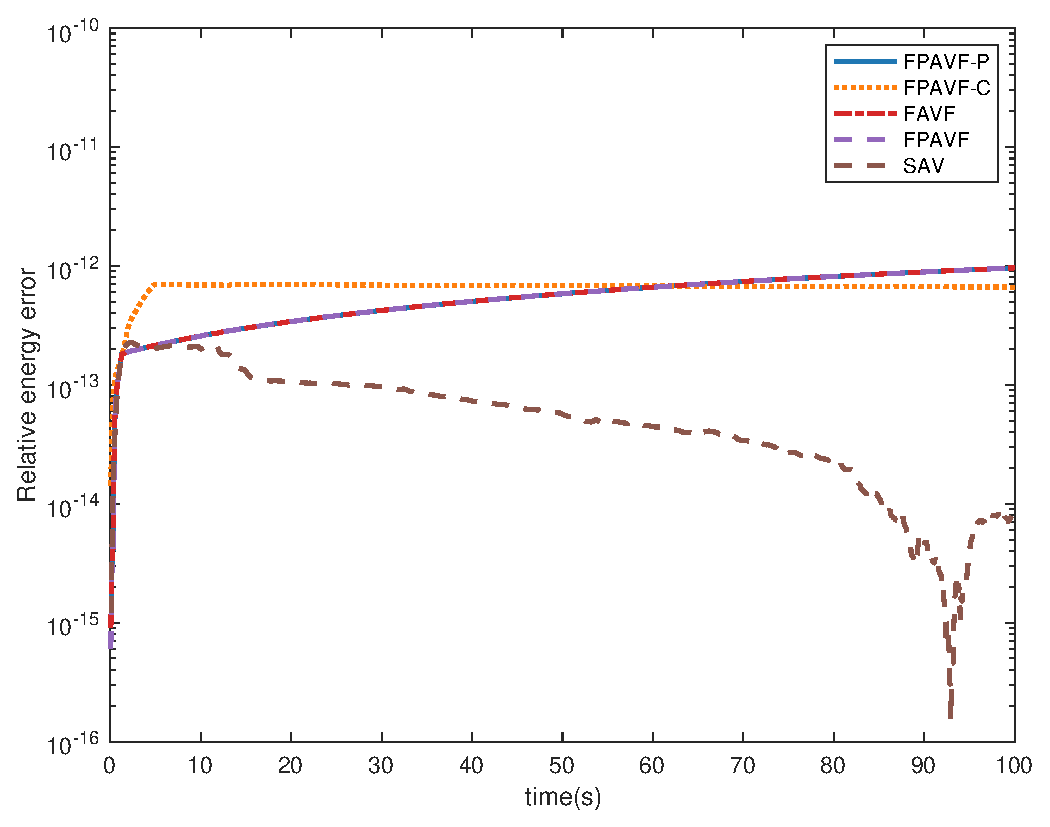
\includegraphics[width=0.3\textwidth]{./figure/exp2_RH1.3.eps}
% %\centerline{($a$) $\alpha=1.3$}
% }\subfigure[$\alpha=1.6$]{ \centering
% 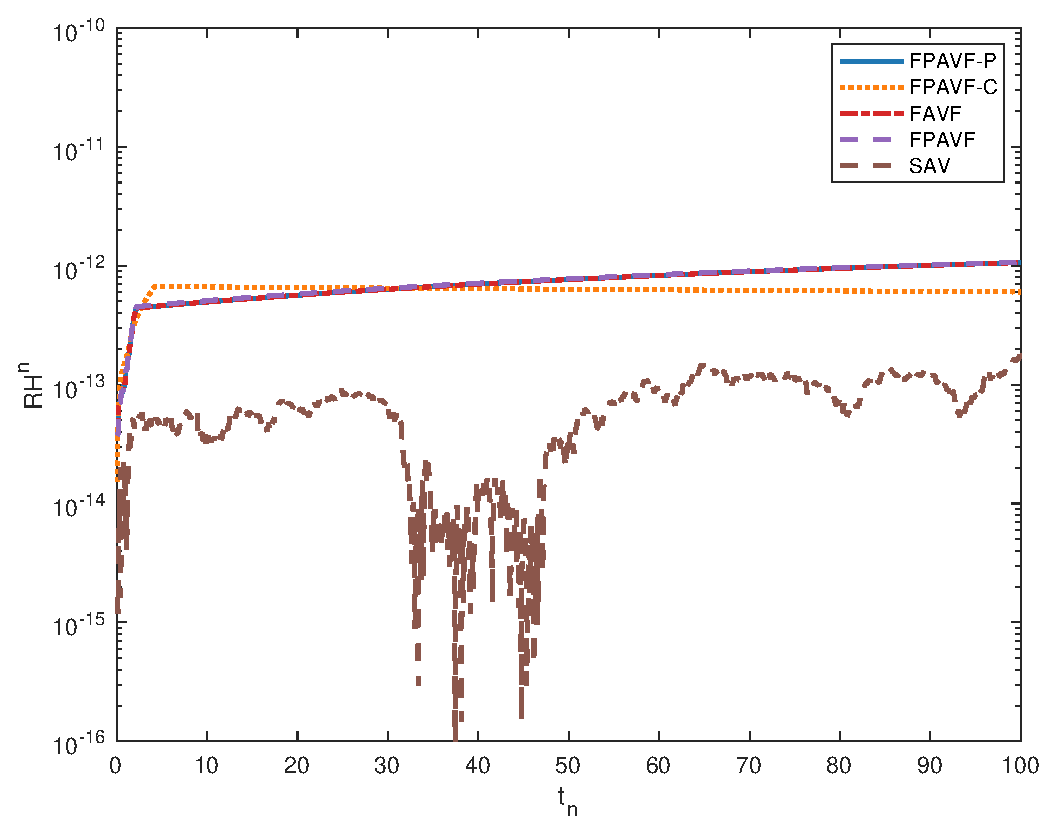
\includegraphics[width=0.3\textwidth]{./figure/exp2_RH1.6.eps}
% %\centerline{($b$) $\alpha=1.6$}
% } \subfigure[$\alpha=1.9$]{ \centering
% 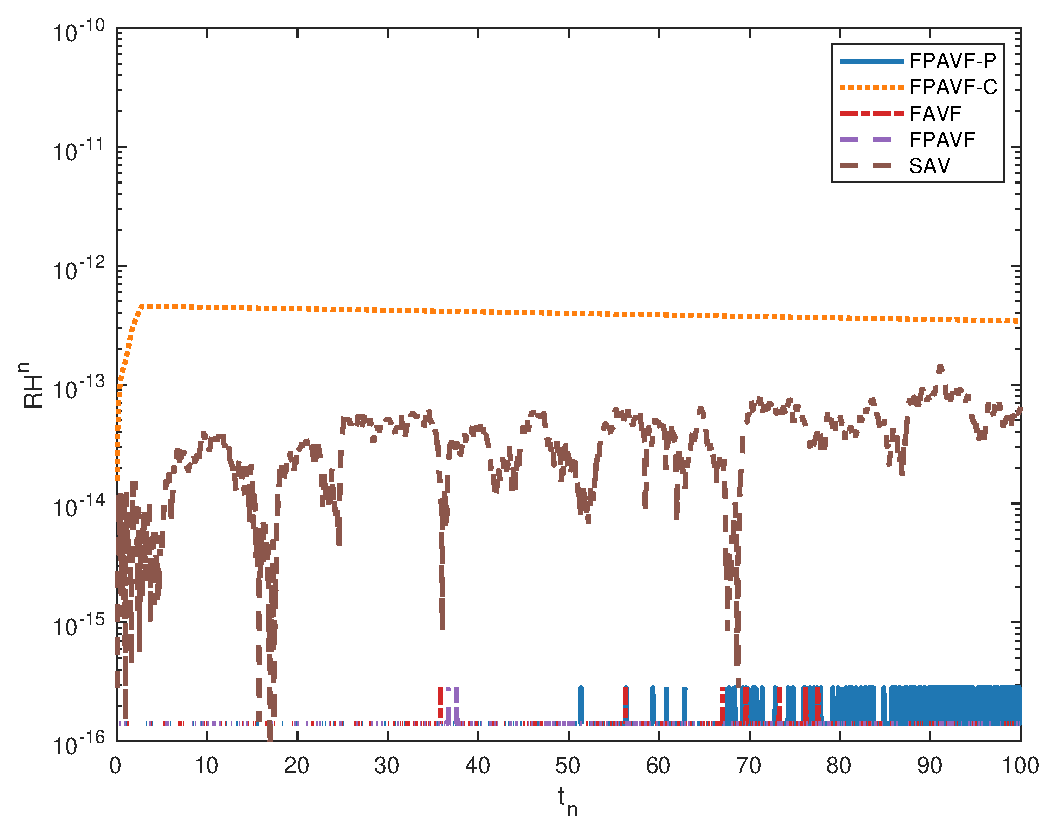
\includegraphics[width=0.3\textwidth]{./figure/exp2_RH1.9.eps}
% %\centerline{($c$) $\alpha=1.9$}
% }\caption{$N = 64,\tau=0.01$时针对不同$\alpha$的相对离散能量误差(例\ref{ex:4}).} \label{fig:12}
% \end{center}
% \end{figure}

% 更详细的比较见表\ref{tab:4-1}-\ref{tab:4-4},我们可以通过观察这些数据得出相同的结论.

% \begin{table}[H]\small
% 	\centering
% 	\caption{当$\alpha=2$时,$t=t_n$处的离散能量$H^n$(例\ref{ex:4}).}
% 	  \begin{tabular}{llllll}
% 	  \toprule
%        $t$   &FAVF   &FPAVF   &FPAVF-C   &SAV   &FPAVF-P\\
% 	  \midrule
% 	  0     & 3.22697078740176 & 3.22697078740176 & 3.22697078740173 & 3.21234862767094 & 3.22697078740176 \\
% 	  10    & 3.22697078740176 & 3.22697078740176 & 3.22697078740168 & 3.21234862767062 & 3.22697078740176 \\
% 	  20    & 3.22697078740176 & 3.22697078740176 & 3.22697078740172 & 3.21234862767066 & 3.22697078740176 \\
% 	  40    & 3.22697078740175 & 3.22697078740176 & 3.22697078740182 & 3.21234862767033 & 3.22697078740176 \\
% 	  60    & 3.22697078740176 & 3.22697078740176 & 3.22697078740191 & 3.21234862767035 & 3.22697078740176 \\
% 	  80    & 3.22697078740176 & 3.22697078740175 & 3.22697078740199 & 3.21234862767073 & 3.22697078740176 \\
% 	  100   & 3.22697078740175 & 3.22697078740176 & 3.22697078740207 & 3.21234862767045 & 3.22697078740176 \\
% 	  \midrule
% 	  \multicolumn{6}{r}{Original energy:~3.22697078976648} \\
% 	  \bottomrule
% 	  \end{tabular}\label{tab:4-1}%
%   \end{table}%


%   % Table generated by Excel2LaTeX from sheet 'Sheet1'
% \begin{table}[H]\small
% 	\centering
% 	\caption{当$\alpha=1.3$时,$t=t_n$处的离散质量$G^n$(例\ref{ex:4}).}
% 	  \begin{tabular}{lllll}
% 	  \toprule
% $t$   &FAVF   &FPAVF   &FPAVF-C   &FPAVF-P\\
% 	  \midrule
% 	  0     & 3.14159297667455 & 3.14159361842152 & 3.14159241227909 & 3.14159265358976 \\
% 	  10    & 3.14160952253933 & 3.13595374862870 & 3.14166505643569 & 3.14159265358963 \\
% 	  20    & 3.14161343543099 & 3.14421089321261 & 3.14158965037808 & 3.14159265358952 \\
% 	  40    & 3.14157539023564 & 3.14362067013654 & 3.14159917106759 & 3.14159265358932 \\
% 	  60    & 3.14150249358846 & 3.14217508702013 & 3.14159868539556 & 3.14159265358912 \\
% 	  80    & 3.14143174175214 & 3.14159826267015 & 3.14158946625201 & 3.14159265358895 \\
% 	  100   & 3.14135672071641 & 3.14328710863969 & 3.14158227319751 & 3.14159265358880 \\
% 	  \midrule
% 	  \multicolumn{5}{r}{Original mass:~3.14159265323701} \\
% 	  \bottomrule
% 	  \end{tabular}\label{tab:4-2}%
%   \end{table}%

%   % Table generated by Excel2LaTeX from sheet 'Sheet1'
% \begin{table}[H]\small
% 	\centering
% 	\caption{当$\alpha=1.6$时,$t=t_n$处的离散质量$G^n$(例\ref{ex:4}).}
% 	  \begin{tabular}{lllll}
% 	  \toprule
% $t$   &FAVF   &FPAVF   &FPAVF-C   &FPAVF-P\\
% 	  \midrule
% 	  0     & 3.14159297668940 & 3.14159361814729 & 3.14159241218683 & 3.14159265358976 \\
% 	  10    & 3.14163389358031 & 3.13754191888209 & 3.14160072631792 & 3.14159265358928 \\
% 	  20    & 3.14161716177523 & 3.14433222488425 & 3.14159044899067 & 3.14159265358919 \\
% 	  40    & 3.14149554093894 & 3.14475213344308 & 3.14160500647197 & 3.14159265358901 \\
% 	  60    & 3.14139997924855 & 3.14288256207779 & 3.14160023436812 & 3.14159265358885 \\
% 	  80    & 3.14127488637752 & 3.14241392600216 & 3.14158768432513 & 3.14159265358871 \\
% 	  100   & 3.14115287766347 & 3.14489331385338 & 3.14159412822417 & 3.14159265358860 \\
% 		\midrule
% 	  \multicolumn{5}{r}{Original mass:~3.14159265323701} \\
% 	  \bottomrule
% 	  \end{tabular}\label{tab:4-3}%
%   \end{table}%

%   % Table generated by Excel2LaTeX from sheet 'Sheet1'
% \begin{table}[H]\small
% 	\centering
% 	\caption{当$\alpha=2$时,$t=t_n$处的离散质量$G^n$(例\ref{ex:4}).}
% 	  \begin{tabular}{lllll}
% 	  \toprule
% $t$   &FAVF   &FPAVF   &FPAVF-C   &FPAVF-P\\
% 	  \midrule
% 	  0     & 3.14159297725470 & 3.14159361919902 & 3.14159241149324 & 3.14159265358976 \\
% 	  10    & 3.14168000260412 & 3.14369215006721 & 3.14160070161208 & 3.14159265358976 \\
% 	  20    & 3.14164544531849 & 3.14521250122401 & 3.14158745249453 & 3.14159265358976 \\
% 	  40    & 3.14150535695500 & 3.14531702832209 & 3.14160031804829 & 3.14159265358976 \\
% 	  60    & 3.14136438511727 & 3.14552013864766 & 3.14159560564481 & 3.14159265358976 \\
% 	  80    & 3.14118013227991 & 3.14739329967543 & 3.14158800109644 & 3.14159265358976 \\
% 	  100   & 3.14101125059928 & 3.15011874273391 & 3.14154787019595 & 3.14159265358976 \\
% 	  \midrule
% 	  \multicolumn{5}{r}{Original mass:~3.14159265323701} \\
% 	  \bottomrule
% 	  \end{tabular}\label{tab:4-4}%
%   \end{table}%
%   最后,分别取$N=128$和$\tau=0.01$,在图\ref{fig:13}-\ref{fig:16}中描述了$\alpha=1.3,1.6,1.99,2$时,波随时间$t$的演变.
%   我们可以观察到,阶数$\alpha$将显著影响波的形状,当$\alpha$变大时,波的形状变化更快.具体地说,当$\alpha \rightarrow 2$时,
%   数值解收敛于经典非线性Schr{\"o}dinger波动方程,见\cite{zhangConservativeNumericalScheme2003,liCompactFiniteDifference2012,wangAnalysisNewConservative2006}.
%   \begin{figure}[H]
% 	\begin{center}
% 	 \subfigure[$t=0s$]{ \centering
% 	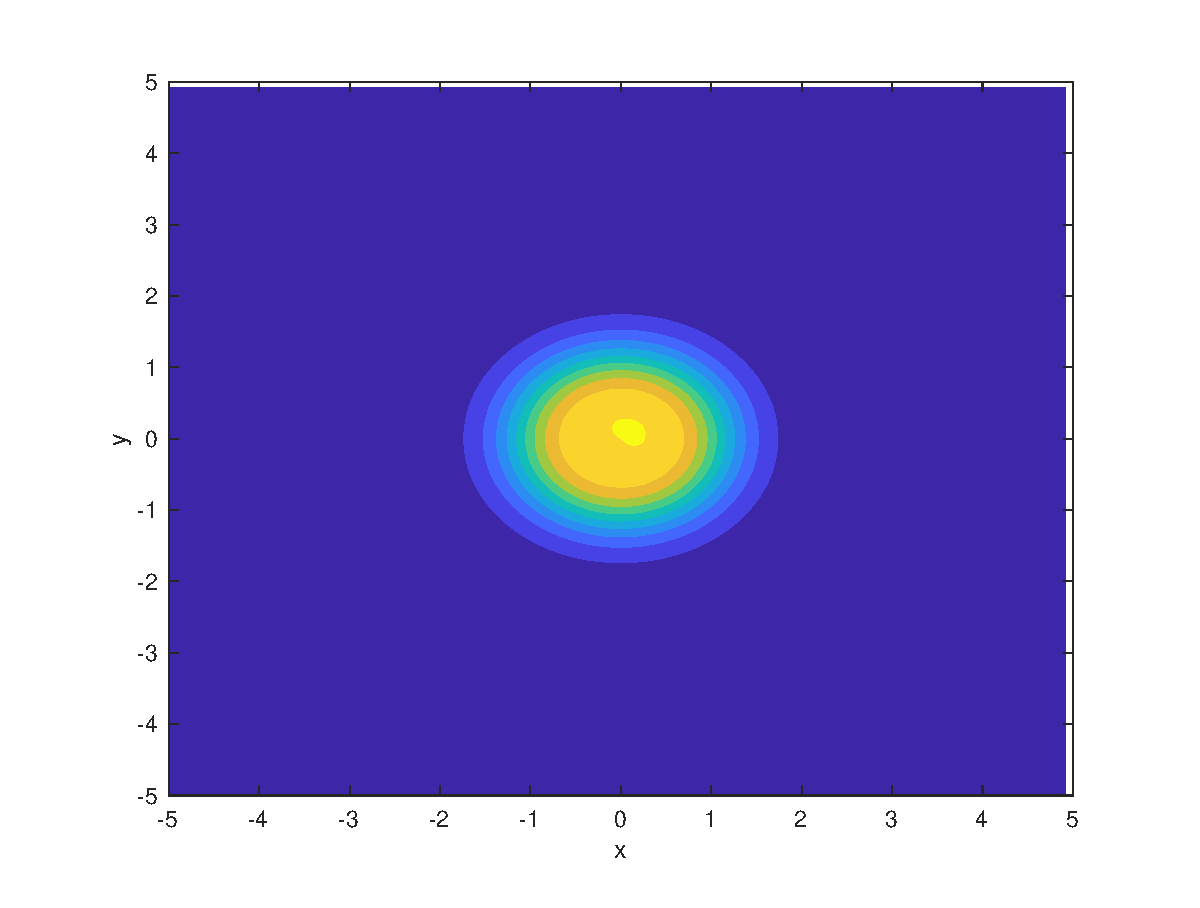
\includegraphics[width=0.3\textwidth]{./figure/exp2_contour3_p0.eps}
% 	}\subfigure[$t=1s$]{ \centering
% 	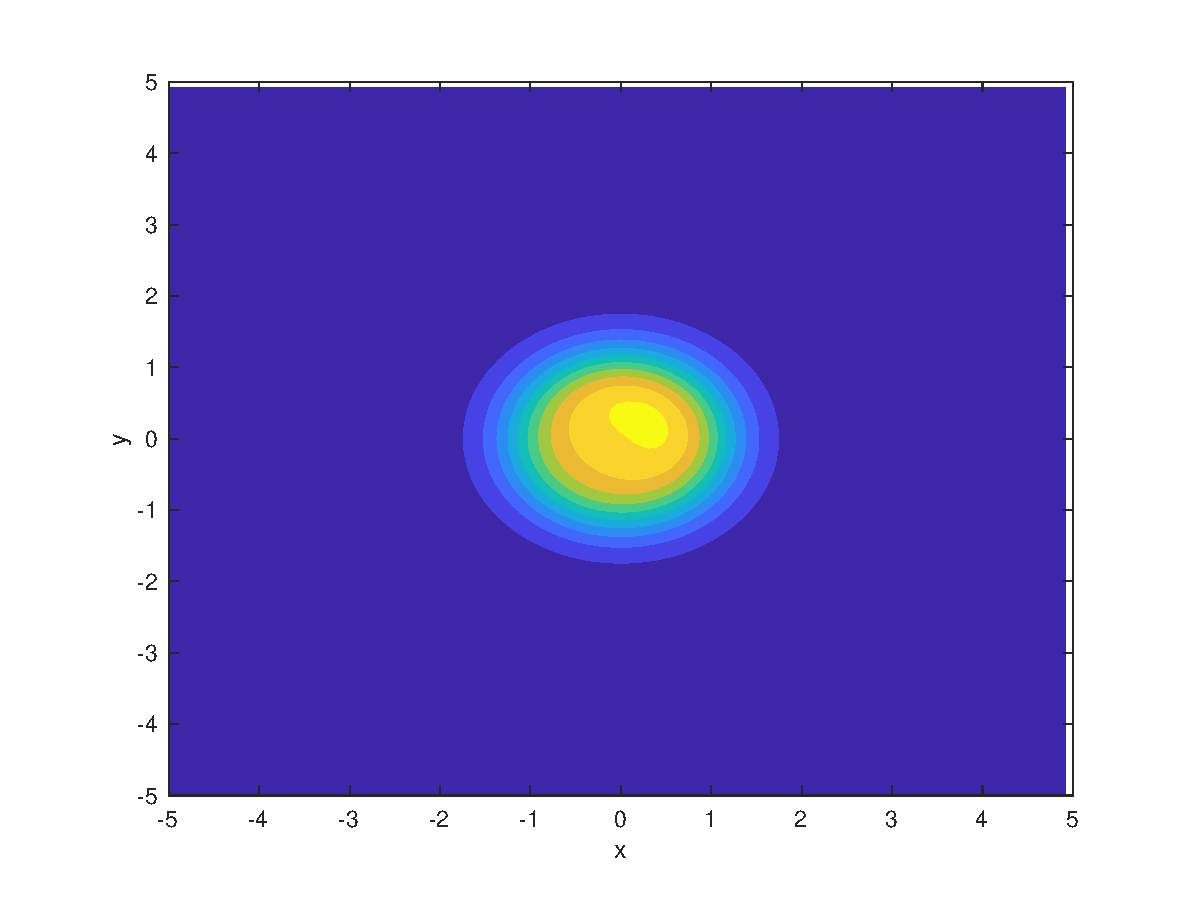
\includegraphics[width=0.3\textwidth]{./figure/exp2_contour3_p1.eps}
% 	} \subfigure[$t=5s$]{ \centering
% 	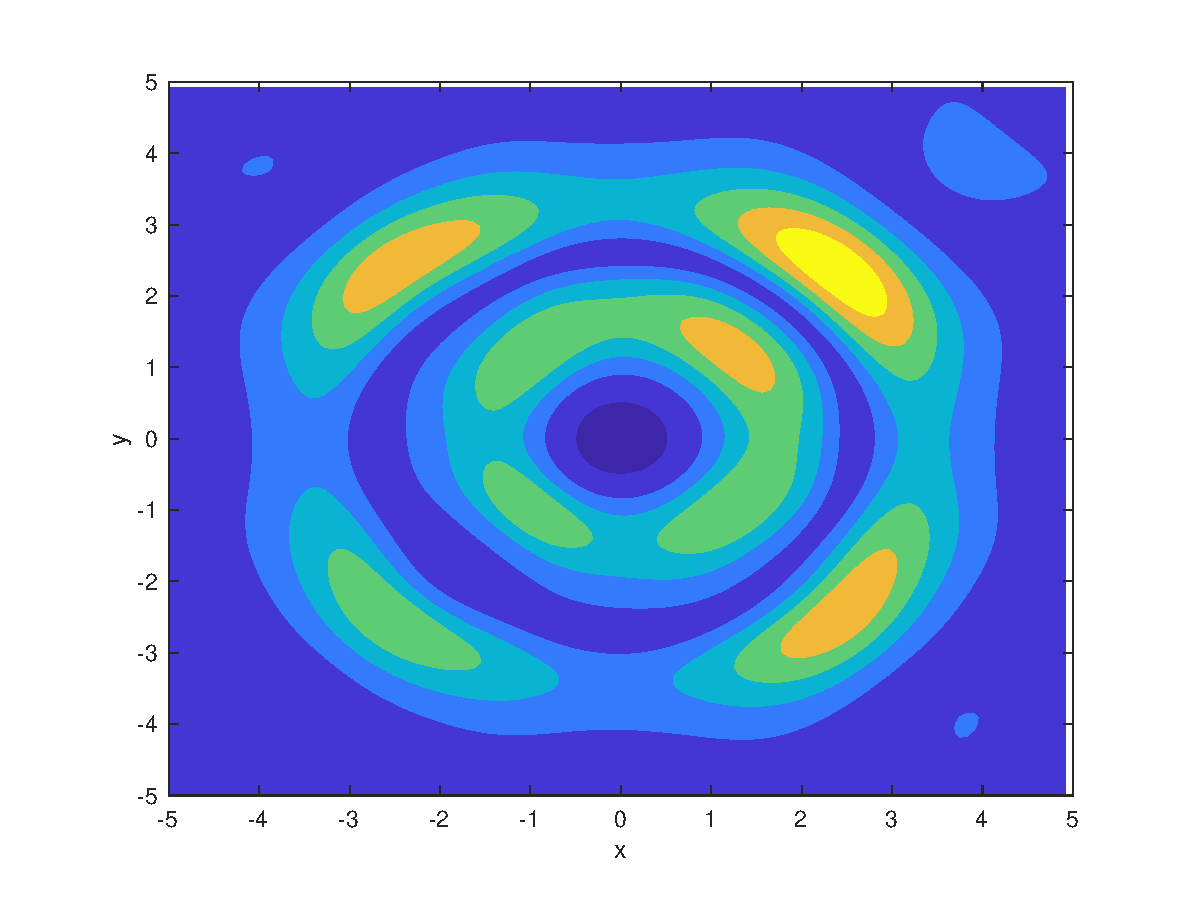
\includegraphics[width=0.3\textwidth]{./figure/exp2_contour3_p5.eps}
% 	}\\
% 	\subfigure[$t=10s$]{ \centering
% 	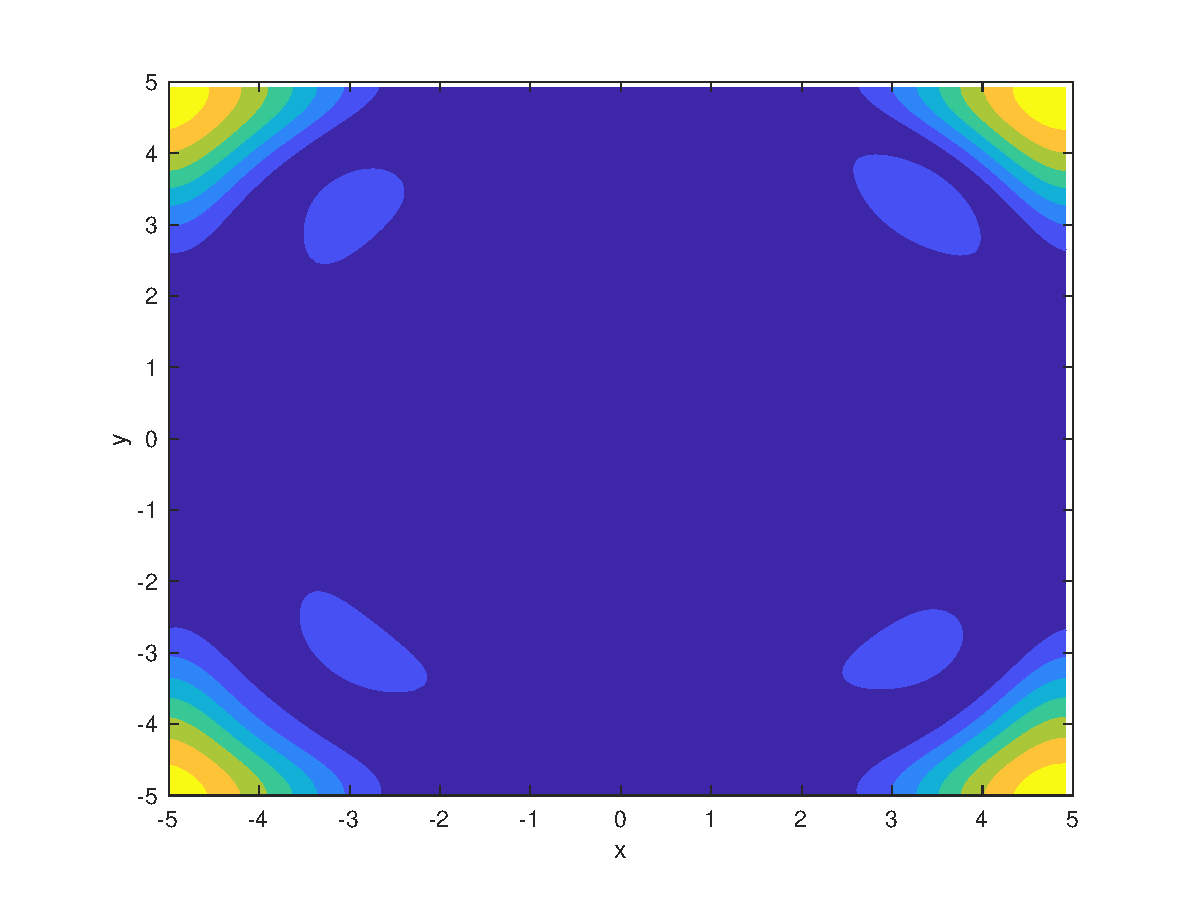
\includegraphics[width=0.3\textwidth]{./figure/exp2_contour3_p10.eps}
% 	}\subfigure[$t=50s$]{ \centering
% 	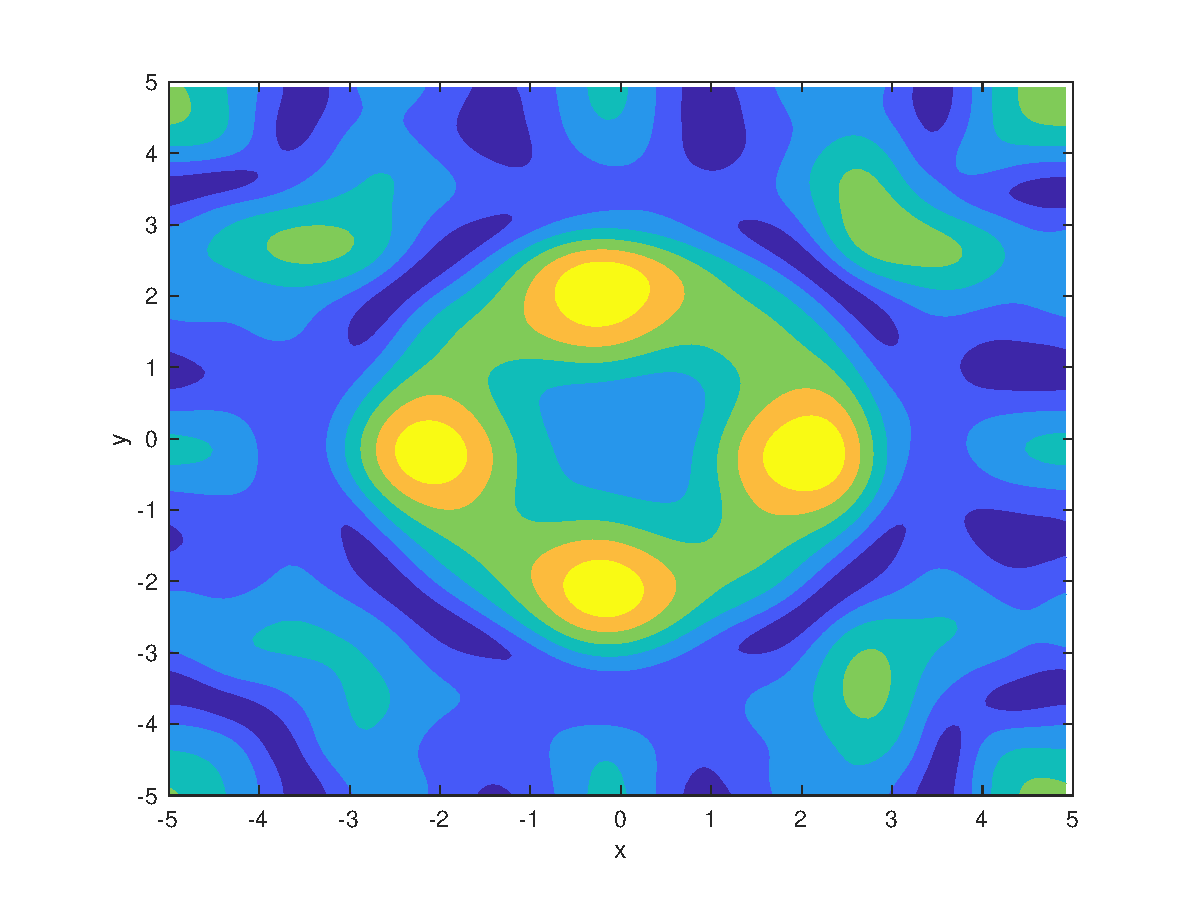
\includegraphics[width=0.3\textwidth]{./figure/exp2_contour3_p50.eps}
% 	} \subfigure[$t=100s$]{ \centering
% 	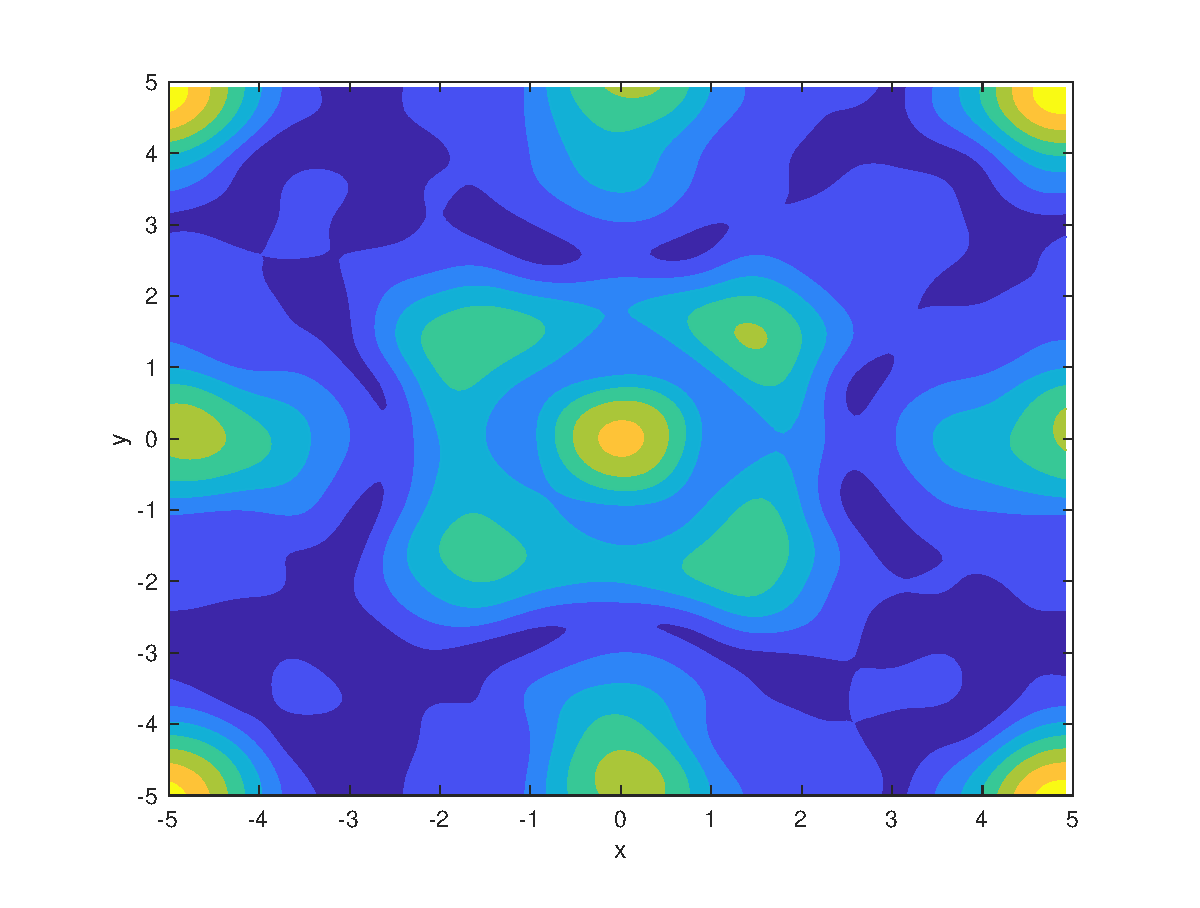
\includegraphics[width=0.3\textwidth]{./figure/exp2_contour3_p100.eps}
% 	}\caption{$\alpha=1.3$时波传播图(例\ref{ex:4})}\label{fig:13}
% 	\end{center}
% 	\end{figure}
% \begin{figure}[H]
% 	\begin{center}
% 	 \subfigure[$t=0s$]{ \centering
% 	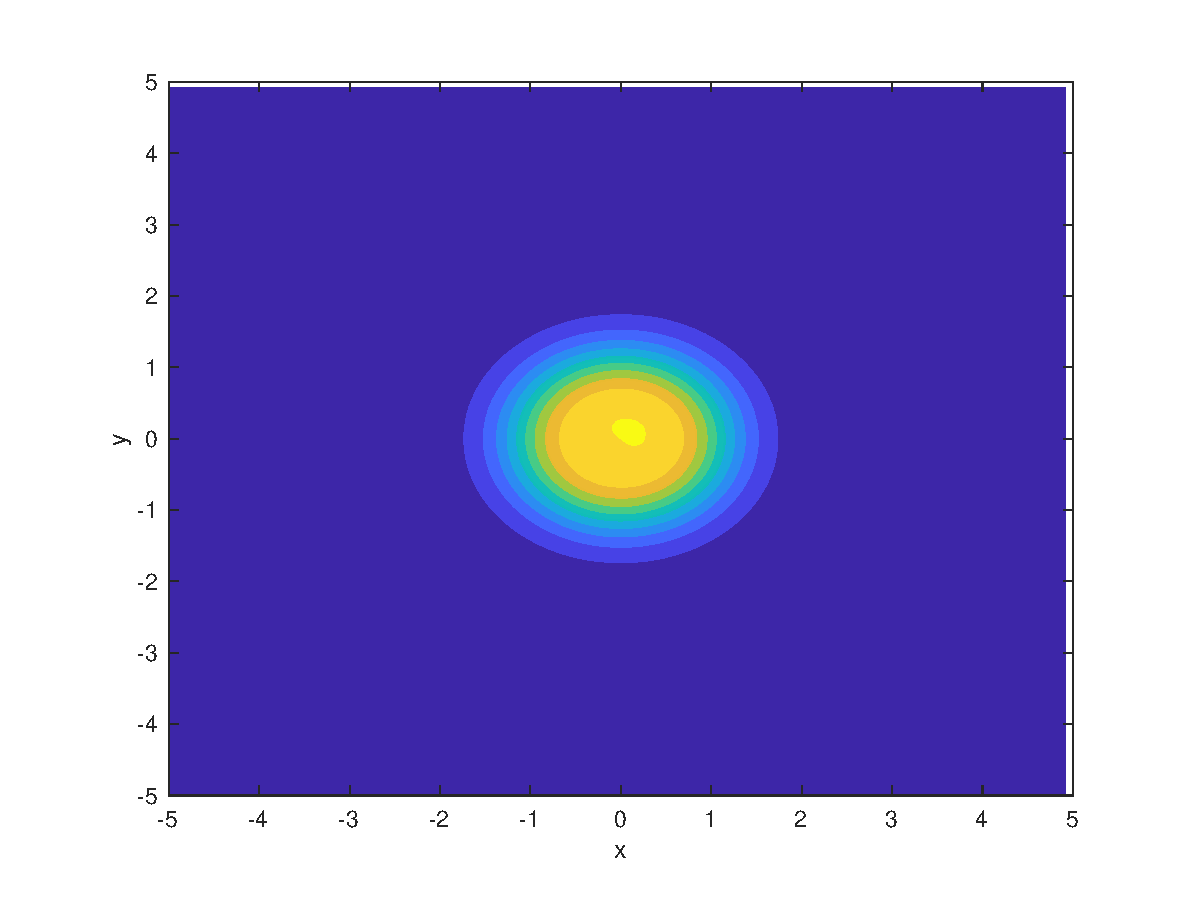
\includegraphics[width=0.3\textwidth]{./figure/exp2_contour6_p0.eps}
% 	}\subfigure[$t=1s$]{ \centering
% 	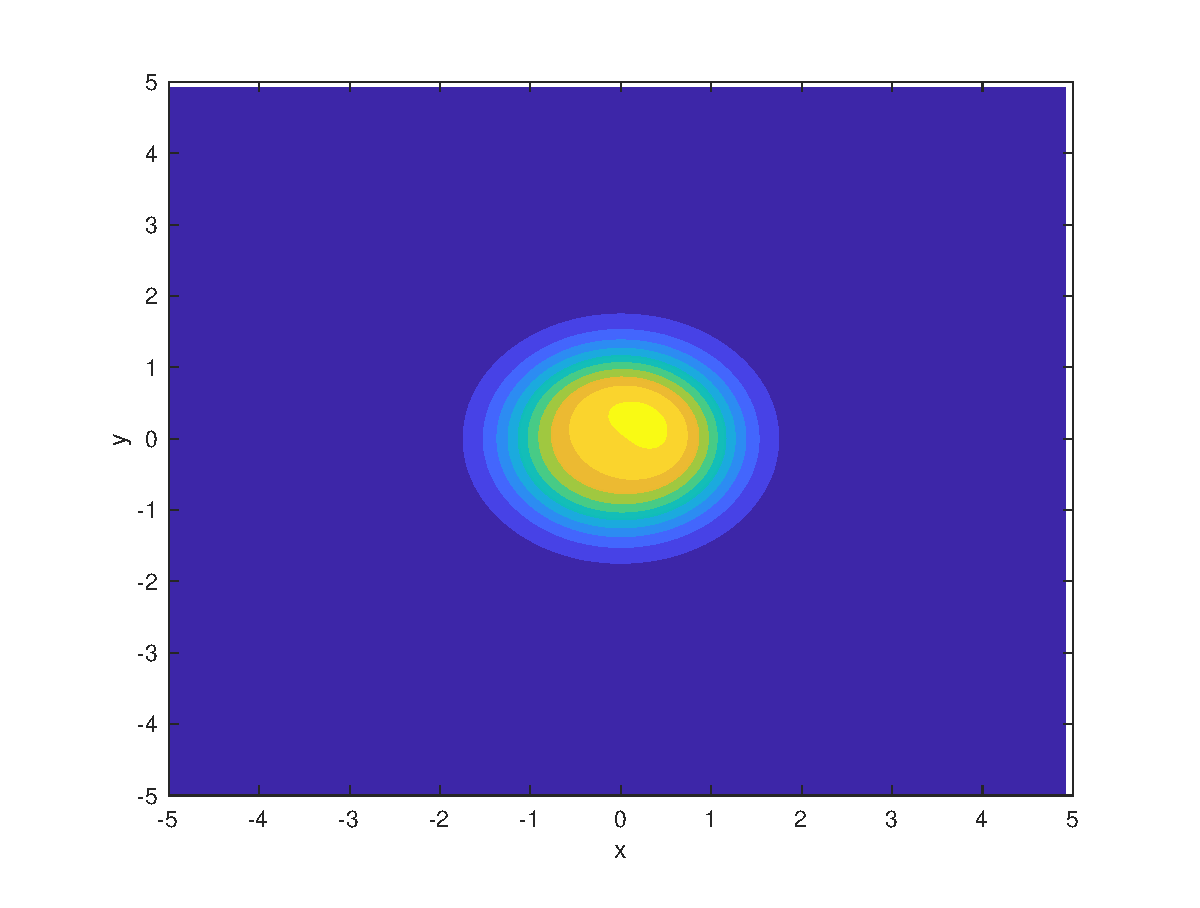
\includegraphics[width=0.3\textwidth]{./figure/exp2_contour6_p1.eps}
% 	} \subfigure[$t=5s$]{ \centering
% 	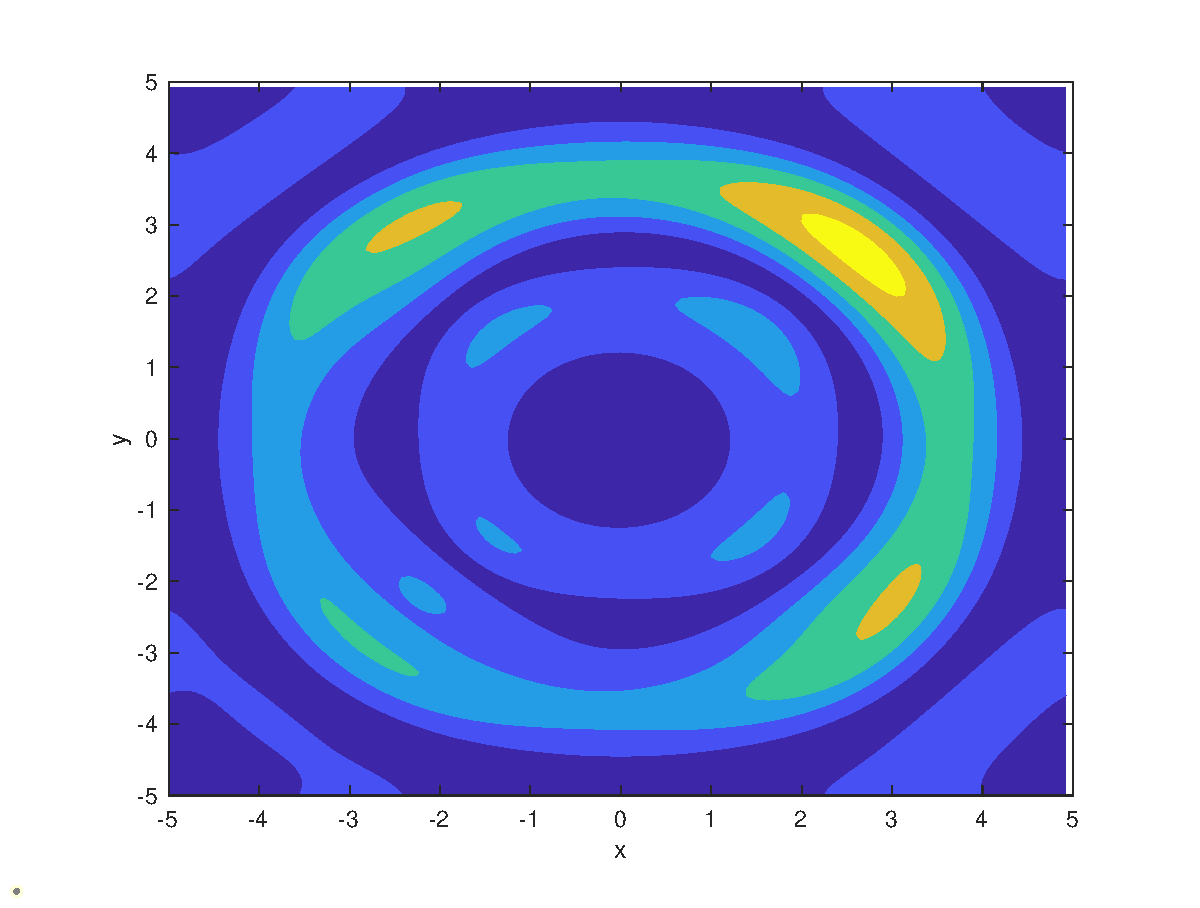
\includegraphics[width=0.3\textwidth]{./figure/exp2_contour6_p5.eps}
% 	}\\
% 	\subfigure[$t=10s$]{ \centering
% 	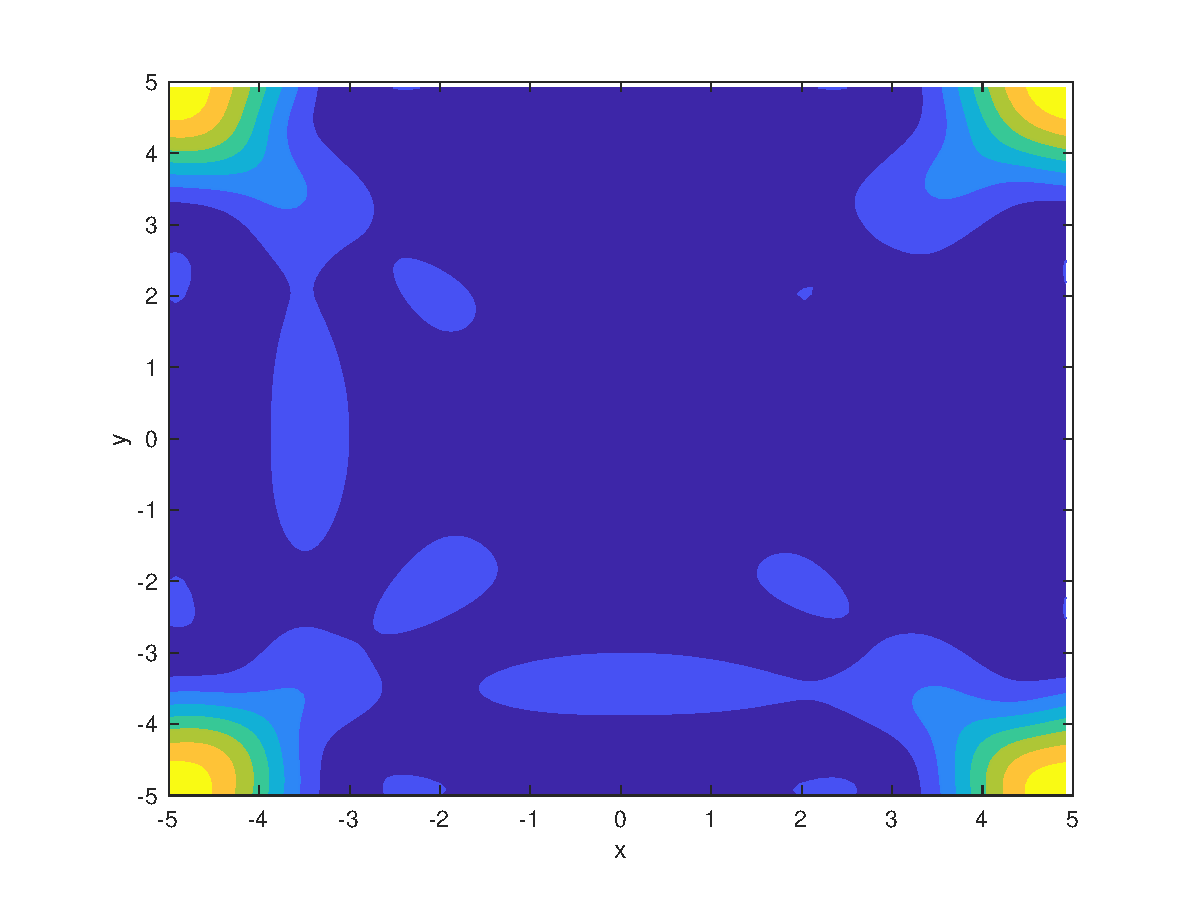
\includegraphics[width=0.3\textwidth]{./figure/exp2_contour6_p10.eps}
% 	}\subfigure[$t=50s$]{ \centering
% 	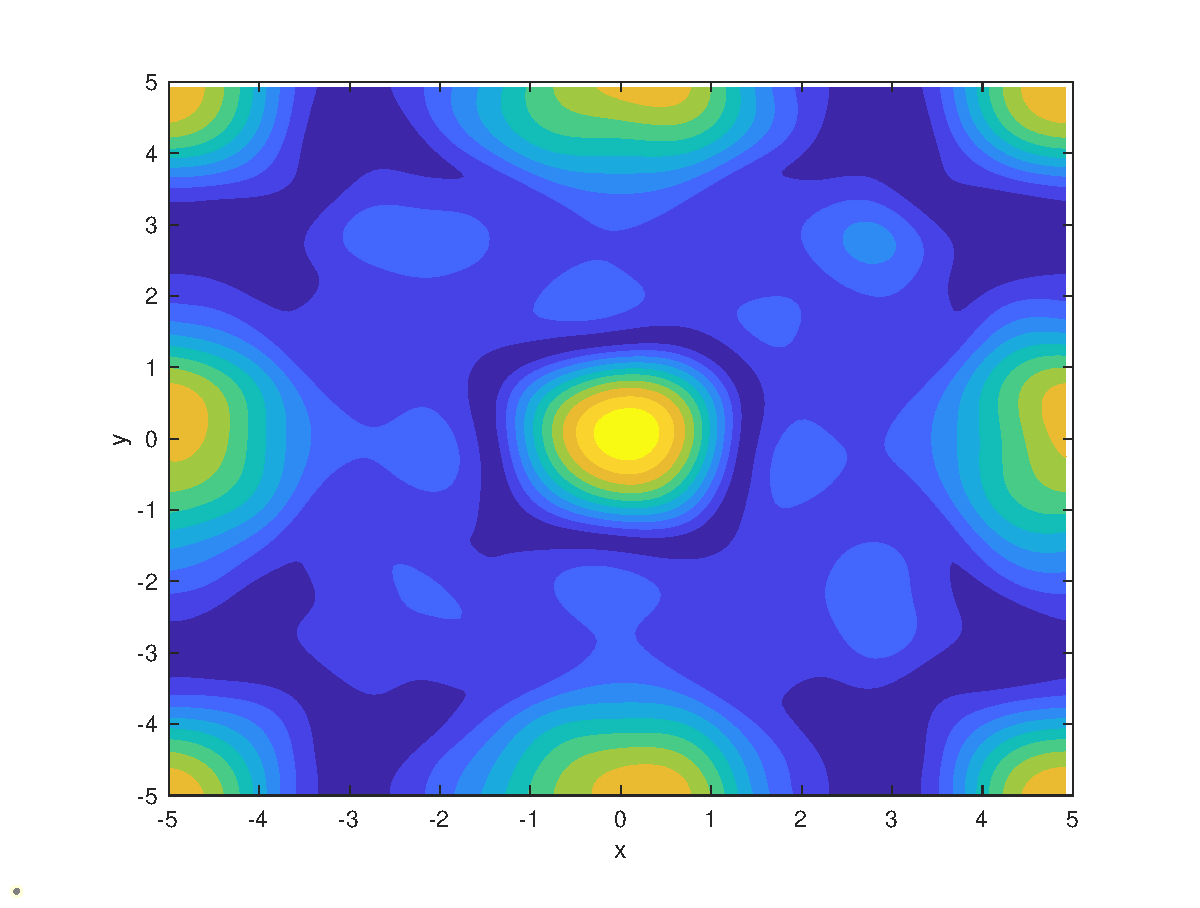
\includegraphics[width=0.3\textwidth]{./figure/exp2_contour6_p50.eps}
% 	} \subfigure[$t=100s$]{ \centering
% 	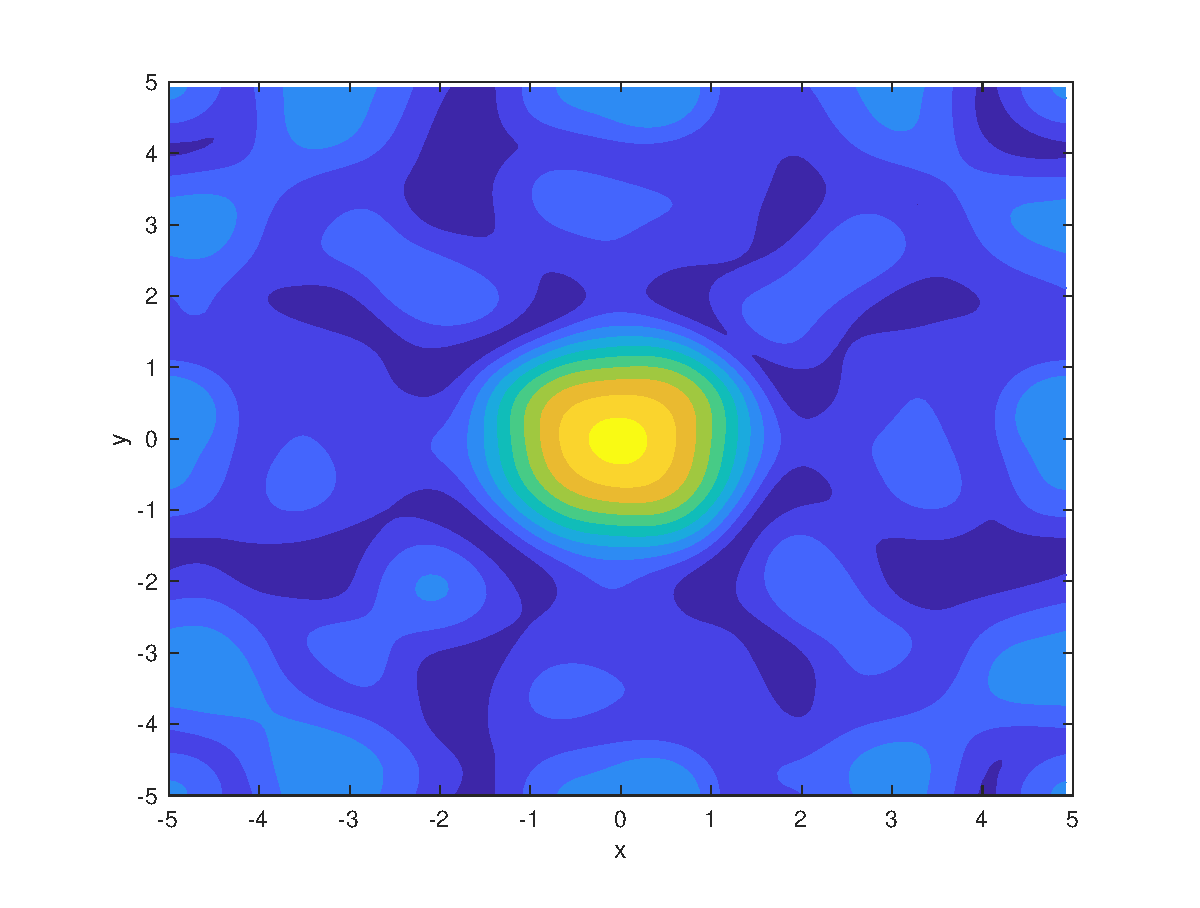
\includegraphics[width=0.3\textwidth]{./figure/exp2_contour6_p100.eps}
% 	}\caption{$\alpha=1.6$时波传播图(例\ref{ex:4})}\label{fig:14}
% 	\end{center}
% 	\end{figure}
% \begin{figure}[H]
% 	\begin{center}
% 	 \subfigure[$t=0s$]{ \centering
% 	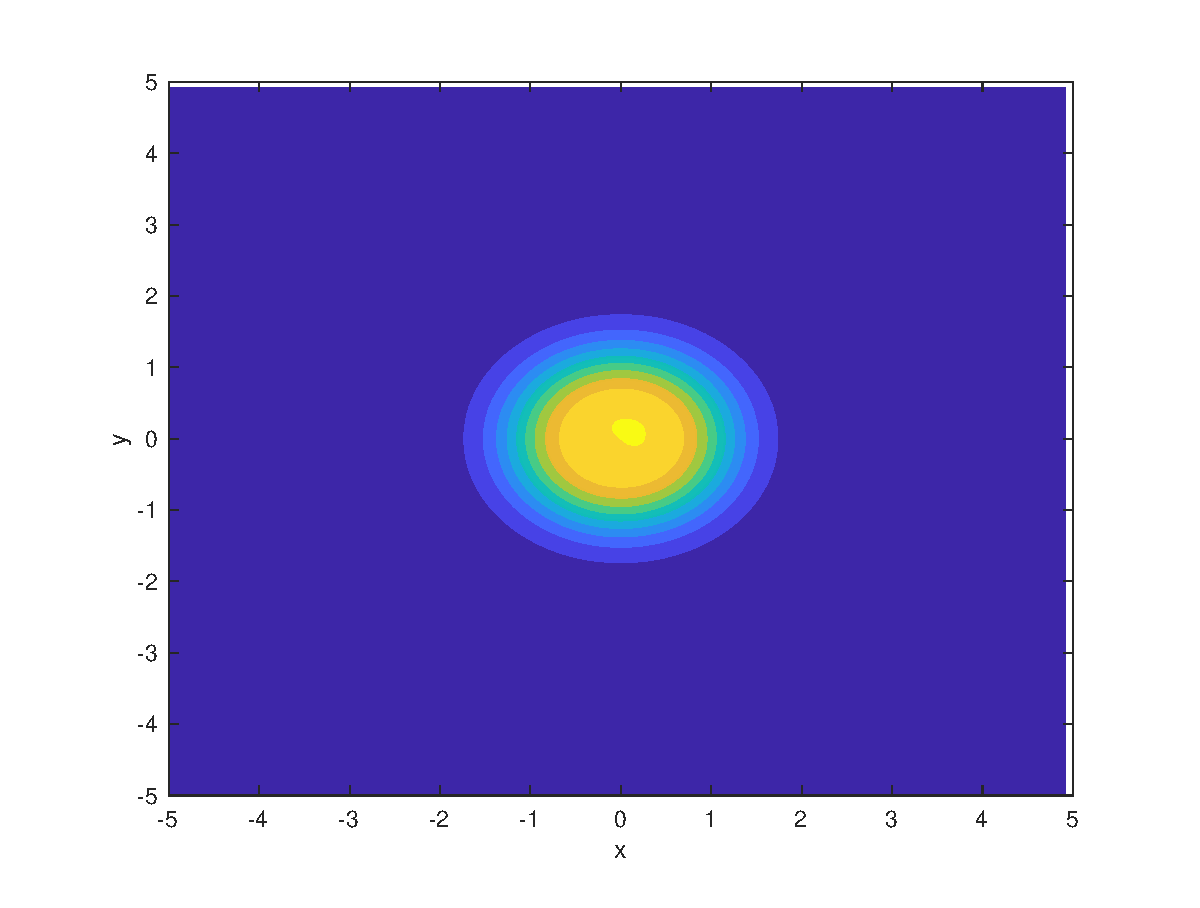
\includegraphics[width=0.3\textwidth]{./figure/exp2_contour99_p0.eps}
% 	}\subfigure[$t=1s$]{ \centering
% 	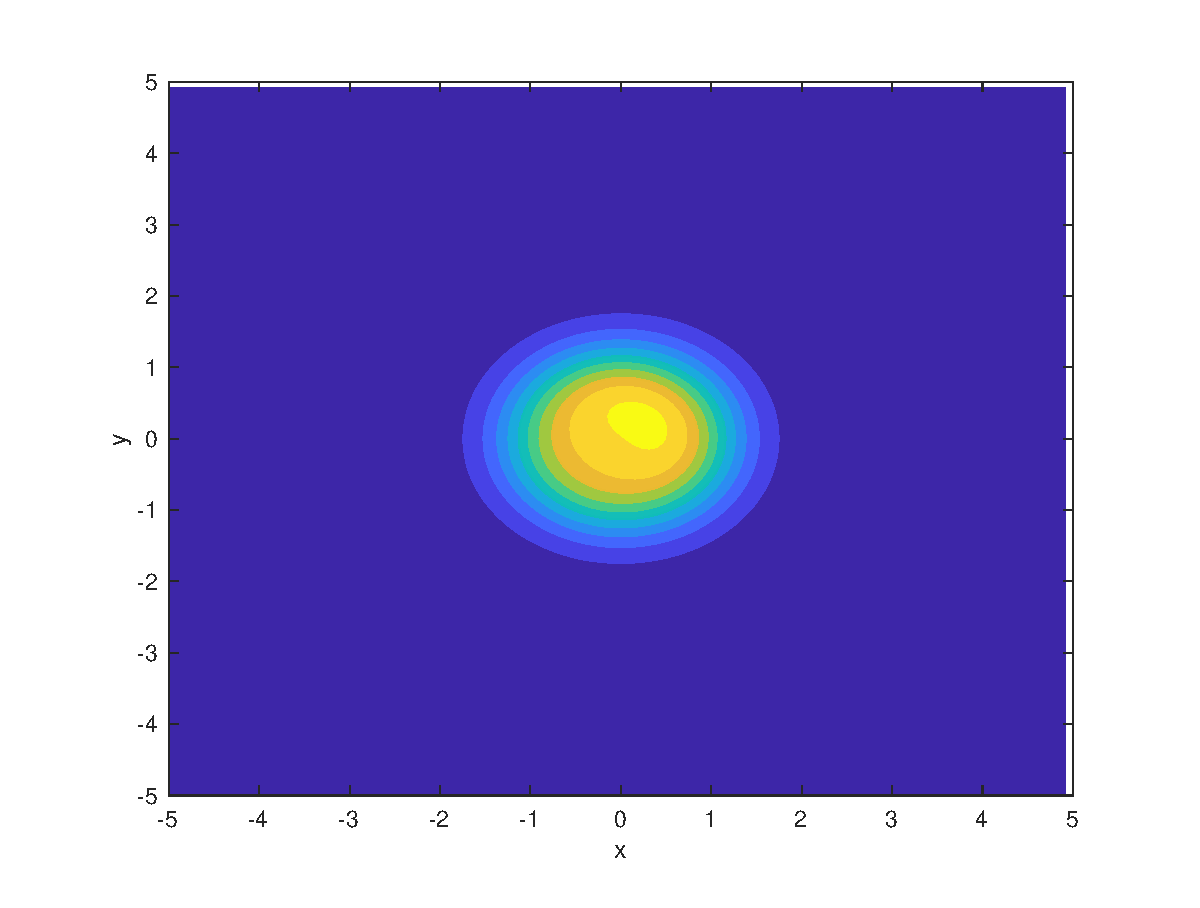
\includegraphics[width=0.3\textwidth]{./figure/exp2_contour99_p1.eps}
% 	} \subfigure[$t=5s$]{ \centering
% 	\includegraphics[width=0.3\textwidth]{./figure/exp2_contour99_p5.eps}
% 	}\\
% 	\subfigure[$t=10s$]{ \centering
% 	\includegraphics[width=0.3\textwidth]{./figure/exp2_contour99_p10.eps}
% 	}\subfigure[$t=50s$]{ \centering
% 	\includegraphics[width=0.3\textwidth]{./figure/exp2_contour99_p50.eps}
% 	} \subfigure[$t=100s$]{ \centering
% 	\includegraphics[width=0.3\textwidth]{./figure/exp2_contour99_p100.eps}
% 	}\caption{$\alpha=1.99$时波传播图(例\ref{ex:4})}\label{fig:15}
% 	\end{center}
% 	\end{figure}

% %---------------------------------------------------------------------------------------------------------------------------
% \begin{figure}[H]
% 	\begin{center}
% 	 \subfigure[$t=0s$]{ \centering
% 	\includegraphics[width=0.3\textwidth]{./figure/exp2_contour2_p0.eps}
% 	}\subfigure[$t=1s$]{ \centering
% 	\includegraphics[width=0.3\textwidth]{./figure/exp2_contour2_p1.eps}
% 	} \subfigure[$t=5s$]{ \centering
% 	\includegraphics[width=0.3\textwidth]{./figure/exp2_contour2_p5.eps}
% 	}\\
% 	\subfigure[$t=10s$]{ \centering
% 	\includegraphics[width=0.3\textwidth]{./figure/exp2_contour2_p10.eps}
% 	}\subfigure[$t=50s$]{ \centering
% 	\includegraphics[width=0.3\textwidth]{./figure/exp2_contour2_p50.eps}
% 	} \subfigure[$t=100s$]{ \centering
% 	\includegraphics[width=0.3\textwidth]{./figure/exp2_contour2_p100.eps}
% 	}\caption{$\alpha=2$时波传播图(例\ref{ex:4})}\label{fig:16}
% 	\end{center}
% 	\end{figure}
